%
% Main document
% ===========================================================================
% This is part of the document "Project documentation template".
% Authors: brd3, kaa1
%

%---------------------------------------------------------------------------
\documentclass[
	a4paper,					% paper format
	11pt,							% fontsize
	twoside,					% double-sided
	openright,				% begin new chapter on right side
	notitlepage,			% use no standard title page
	parskip=half,			% set paragraph skip to half of a line
]{scrreprt}					% KOMA-script report
%---------------------------------------------------------------------------

\raggedbottom
\KOMAoptions{cleardoublepage=plain}			% Add header and footer on blank pages


% Load Standard Packages:
%---------------------------------------------------------------------------
\usepackage[standard-baselineskips]{cmbright}

\usepackage[ngerman,english]{babel}										% english hyphenation
%\usepackage[latin1]{inputenc}  							% Unix/Linux - load extended character set (ISO 8859-1)
\usepackage[ansinew]{inputenc}  							% Windows - load extended character set (ISO 8859-1)
\usepackage[T1]{fontenc}											% hyphenation of words with �,� and �
\usepackage{textcomp}													% additional symbols
\usepackage{ae}																% better resolution of Type1-Fonts 
\usepackage{fancyhdr}													% simple manipulation of header and footer 
\usepackage{etoolbox}													% color manipulation of header and footer
\usepackage{graphicx}                      		% integration of images
\usepackage{float}														% floating objects
\usepackage{caption}													% for captions of figures and tables
\usepackage{booktabs}													% package for nicer tables
\usepackage{tocvsec2}													% provides means of controlling the sectional numbering
%---------------------------------------------------------------------------

% Load Math Packages
%---------------------------------------------------------------------------
\usepackage{amsmath}                    	   	% various features to facilitate writing math formulas
\usepackage{amsthm}                       	 	% enhanced version of latex's newtheorem
\usepackage{amsfonts}                      		% set of miscellaneous TeX fonts that augment the standard CM
\usepackage{amssymb}													% mathematical special characters
\usepackage{exscale}													% mathematical size corresponds to textsize
%---------------------------------------------------------------------------

% Package to facilitate placement of boxes at absolute positions
%---------------------------------------------------------------------------
\usepackage[absolute]{textpos}
\setlength{\TPHorizModule}{1mm}
\setlength{\TPVertModule}{1mm}
%---------------------------------------------------------------------------					
			
% Definition of Colors
%---------------------------------------------------------------------------
\RequirePackage{color}                          % Color (not xcolor!)
\definecolor{linkblue}{rgb}{0,0,0.8}            % Standard
\definecolor{darkblue}{rgb}{0,0.08,0.45}        % Dark blue
\definecolor{bfhgrey}{rgb}{0.41,0.49,0.57}      % BFH grey
%\definecolor{linkcolor}{rgb}{0,0,0.8}     			% Blue for the web- and cd-version!
\definecolor{linkcolor}{rgb}{0,0,0}        			% Black for the print-version!
%---------------------------------------------------------------------------

% Hyperref Package (Create links in a pdf)
%---------------------------------------------------------------------------
\usepackage[
	pdftex,ngerman,bookmarks,plainpages=false,pdfpagelabels,
	backref = {false},										% No index backreference
	colorlinks = {true},                  % Color links in a PDF
	hypertexnames = {true},               % no failures "same page(i)"
	bookmarksopen = {true},               % opens the bar on the left side
	bookmarksopenlevel = {0},             % depth of opened bookmarks
	pdftitle = {Template f�r Bachelor Thesis},	   	% PDF-property
	pdfauthor = {brd3},        					  % PDF-property
	pdfsubject = {LaTeX Template},        % PDF-property
	linkcolor = {linkcolor},              % Color of Links
	citecolor = {linkcolor},              % Color of Cite-Links
	urlcolor = {linkcolor},               % Color of URLs
]{hyperref}
%---------------------------------------------------------------------------

% Set up page dimension
%---------------------------------------------------------------------------
\usepackage{geometry}
\geometry{
	a4paper,
	left=33mm, %28
	right=20mm, %15
	top=30mm,
	headheight=20mm,
	headsep=10mm,
	textheight=242mm,
	footskip=15mm
}
%---------------------------------------------------------------------------

% Makeindex Package
%---------------------------------------------------------------------------
\usepackage{makeidx}                         		% To produce index
\makeindex                                    	% Index-Initialisation
%---------------------------------------------------------------------------

% Glossary Package
%---------------------------------------------------------------------------
% the glossaries package uses makeindex
% if you use TeXnicCenter do the following steps:
%  - Goto "Ausgabeprofile definieren" (ctrl + F7)
%  - Select the profile "LaTeX => PDF"
%  - Add in register "Nachbearbeitung" a new "Postprozessoren" point named Glossar
%  - Select makeindex.exe in the field "Anwendung" ( ..\MiKTeX x.x\miktex\bin\makeindex.exe )
%  - Add this [ -s "%tm.ist" -t "%tm.glg" -o "%tm.gls" "%tm.glo" ] in the field "Argumente"
%
% for futher informations go to http://ewus.de/tipp-1029.html
%---------------------------------------------------------------------------
\usepackage[nonumberlist]{glossaries}
\makeglossaries

\newglossaryentry{BibTeX}{name={BibTeX},description={Program for the creation of 	bibliographical references and directories in \TeX or \LaTeX documents}}
\newglossaryentry{Index}{name={Index},description={Index with keywords from text}}



%---------------------------------------------------------------------------

\usepackage{pdfpages}

% Intro:
%---------------------------------------------------------------------------
\begin{document}                              	% Start Document
\settocdepth{section}														% Set depth of toc
\pagenumbering{roman}														
%---------------------------------------------------------------------------

\providecommand{\heading}{Utility AI Tool for Unity}		%  Insert Title of Thesis here					% Titel der Arbeit aus Datei titel.tex lesen
\providecommand{\versionnumber}{1.0.0}			%  Hier die aktuelle Versionsnummer eingeben
\providecommand{\versiondate}{14.06.2023}		%  Hier das Datum der aktuellen Version eingeben				% Versionsnummer und -datum aus Datei version.tex lesen

% Set up header and footer
%---------------------------------------------------------------------------
\makeatletter
\patchcmd{\@fancyhead}{\rlap}{\color{bfhgrey}\rlap}{}{}		% new color of header
\patchcmd{\@fancyfoot}{\rlap}{\color{bfhgrey}\rlap}{}{}		% new color of footer
\makeatother

\fancyhf{}																		% clean all fields
\fancypagestyle{plain}{												% new definition of plain style	
	\fancyfoot[OR,EL]{\footnotesize \thepage} 	% footer right part --> page number
	\fancyfoot[OL,ER]{\footnotesize \heading, Version \versionnumber, \versiondate}	% footer even page left part 
}

\renewcommand{\chaptermark}[1]{\markboth{\thechapter.  #1}{}}
\renewcommand{\headrulewidth}{0pt}				% no header stripline
\renewcommand{\footrulewidth}{0pt} 				% no bottom stripline

\pagestyle{plain}
%---------------------------------------------------------------------------


% Title Page and Abstract
%---------------------------------------------------------------------------
%%
% Project documentation template
% ===========================================================================
% This is part of the document "Project documentation template".
% Authors: brd3, kaa1
%

\begin{titlepage}


% BFH-Logo absolute placed at (28,12) on A4 and picture (16:9 or 15cm x 8.5cm)
% Actually not a realy satisfactory solution but working.
%---------------------------------------------------------------------------
\setlength{\unitlength}{1mm}
\begin{textblock}{20}[0,0](28,12)
	
\includegraphics[scale=1.0]{images/BFH_Logo_B.png}
\end{textblock}

% Institution / titel / subtitel / authors / experts:
%---------------------------------------------------------------------------
\begin{flushleft}

\vspace*{21mm}

\fontsize{26pt}{40pt}\selectfont 
\heading				\\							% Read heading from file leader/title.tex
\vspace{2mm}

\fontsize{16pt}{24pt}\selectfont\vspace{0.3em}
Place your subheading here 			\\				% Insert subheading
\vspace{5mm}

\fontsize{10pt}{12pt}\selectfont
\textbf{Description of thesis (semester- / Bachelor thesis / etc.)} \\		% Insert text
\vspace{7mm}

% Abstract (eingeben):
%---------------------------------------------------------------------------
\begin{textblock}{150}(28,100)
\fontsize{10pt}{12pt}\selectfont
[Insert short text (abstract) if desired] \\ 
This document serves as a template for the compilation of reports according to the guidelines of the BFH. The template is written in LATEX and supports the automatic writing of various directories, references, indexing and glossaries. This small text is a summary of this document with a length of 4 to max. 8 lines. \\ 
The cover picture may be turned on or off in the lines 157/158 of the file template.tex.
\end{textblock}

\begin{textblock}{150}(28,225)
\fontsize{10pt}{17pt}\selectfont
\begin{tabbing}
xxxxxxxxxxxxxxx\=xxxxxxxxxxxxxxxxxxxxxxxxxxxxxxxxxxxxxxxxxxxxxxx \kill
Degree course:	\> [z.B. Electrical and Communication Engineering]	\\		% insert name of degree course
Authors:		\> [Test Peter, M\"uster R\"os\"a]		\\					% insert names
Tutor:	\> [Dr.~Xxxx Xxxx, Dr.~Yyyy Yyyy]		\\							% insert names
Constituent:	\> [Wwwww AG]					\\							% insert names
Experts:		\> [Dr.~Zzzz Zzzz]				\\							% insert names
Date:			\> \versiondate					\\							% read from file leader/version.tex
\end{tabbing}

\end{textblock}
\end{flushleft}

\begin{textblock}{150}(28,280)
\noindent 
\color{bfhgrey}\fontsize{9pt}{10pt}\selectfont
Berner Fachhochschule | Haute \'ecole sp\'ecialis\'ee bernoise | Bern University of Applied Sciences
\color{black}\selectfont
\end{textblock}


\end{titlepage}

%
% ===========================================================================
% EOF
%
		% activate for frontpage without picture
%
% Project documentation template
% ===========================================================================
% This is part of the document "Project documentation template".
% Authors: brd3, kaa1
%

\begin{titlepage}


% BFH-Logo absolute placed at (28,12) on A4 and picture (16:9 or 15cm x 8.5cm)
% Actually not a realy satisfactory solution but working.
%---------------------------------------------------------------------------
\setlength{\unitlength}{1mm}
\begin{textblock}{20}[0,0](33,12)
	
\includegraphics[scale=1.0]{images/BFH_Logo_B.png}
\end{textblock}

%\begin{textblock}{154}(28,48)
%	\begin{picture}(150,2)
%		\put(0,0){\color{bfhgrey}\rule{150mm}{2mm}}
%	\end{picture}
%\end{textblock}

\begin{textblock}{154}[0,0](33,50)
	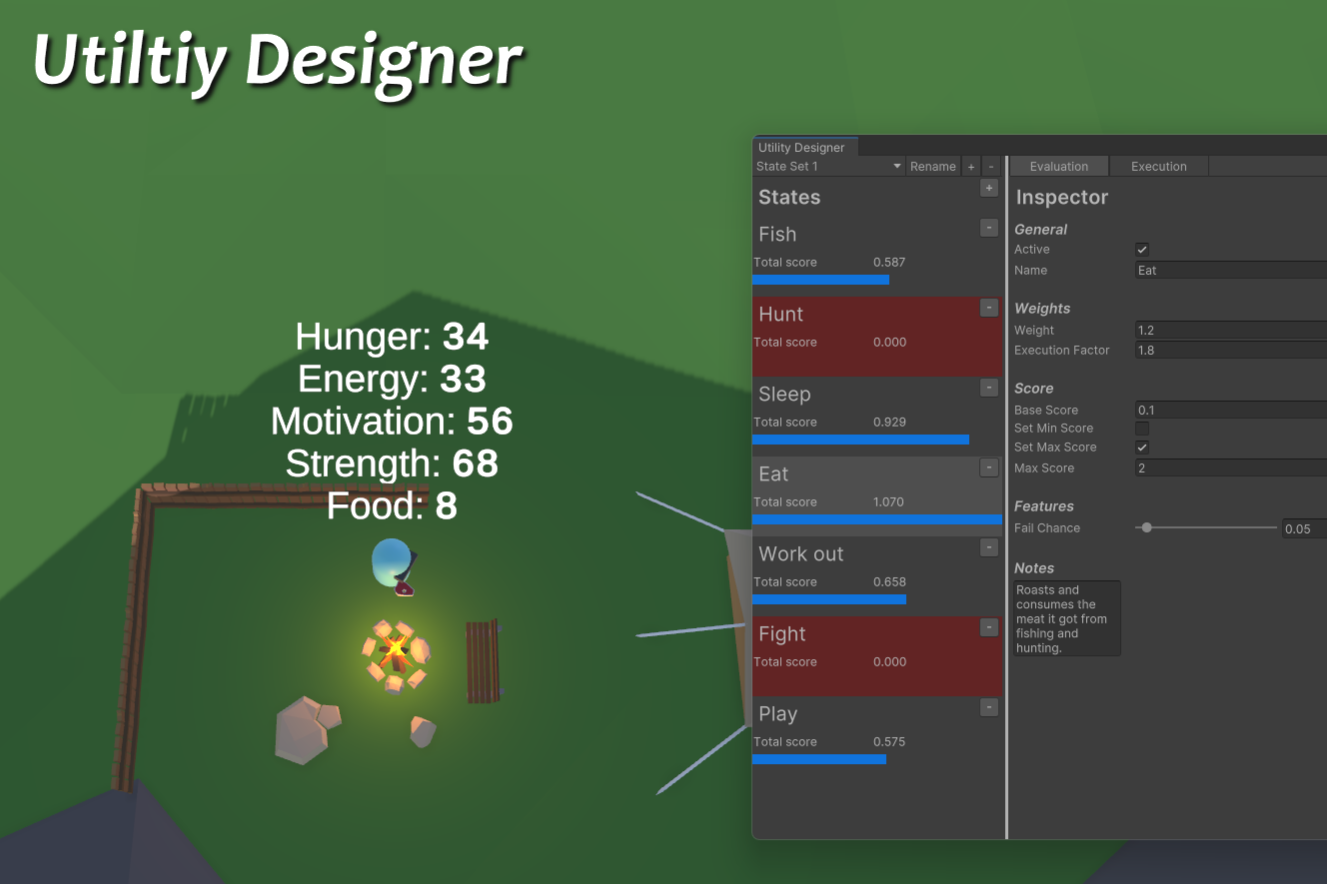
\includegraphics[scale=0.39]{images/title_image.png}			% define cover picture
\end{textblock}

%\begin{textblock}{154}(28,135)
%	\begin{picture}(150,2)
%		\put(0,0){\color{bfhgrey}\rule{150mm}{2mm}}
%	\end{picture}
%\end{textblock}
\color{black}

% Institution / titel / subtitel / authors / experts:
%---------------------------------------------------------------------------
\begin{flushleft}

\vspace*{115mm}

\fontsize{26pt}{28pt}\selectfont 
\heading				\\							% Read heading from file leader/title.tex
\vspace{2mm}

\fontsize{16pt}{20pt}\selectfont\vspace{0.3em}
Utility Designer - Combining Utility AI and Behaviour Trees 			\\	% Insert subheading
\vspace{5mm}

\fontsize{10pt}{12pt}\selectfont
\textbf{Bachelor Thesis} \\		% Insert text
\vspace{3mm}

% Abstract (eingeben):
%---------------------------------------------------------------------------
\begin{textblock}{150}(33,190)
\fontsize{10pt}{12pt}\selectfont
The development of a flexible and intuitive tool for the Unity Asset Store called Utility Designer, which helps to create realistically behaving non-player characters.

\end{textblock}

\begin{textblock}{150}(33,225)
\fontsize{10pt}{17pt}\selectfont
\begin{tabbing}
xxxxxxxxxxxxxxx\=xxxxxxxxxxxxxxxxxxxxxxxxxxxxxxxxxxxxxxxxxxxxxxx \kill
Degree course:	\> Computer Science	\\		% insert name of degree course
Author:		\> K\"aser David		\\					% insert names
Tutor:	\> Dr.~Hudritsch Marcus		\\							% insert names
Constituent:	\> BFH					\\							% insert names
Expert:		\> Studer Harald				\\							% insert names
Date:			\> \versiondate					\\							% read from file leader/version.tex
\end{tabbing}

\end{textblock}
\end{flushleft}

\begin{textblock}{150}(33,280)
\noindent 
\color{bfhgrey}\fontsize{9pt}{10pt}\selectfont
Berner Fachhochschule | Haute \'ecole sp\'ecialis\'ee bernoise | Bern University of Applied Sciences
\color{black}\selectfont
\end{textblock}


\end{titlepage}

%
% ===========================================================================
% EOF
%
		% activate for frontpage with picture
% Control of versions :
% -----------------------------------------------

\begin{textblock}{180}(20,150)
\color{black}
\begin{huge}
Versions
\end{huge}
\vspace{10mm}

\fontsize{10pt}{18pt}\selectfont
\begin{tabbing}
xxxxxxxxxxx\=xxxxxxxxxxxxxxx\=xxxxxxxxxxxxxx\=xxxxxxxxxxxxxxxxxxxxxxxxxxxxxxxxxxxxxxxxxxxxxxx \kill
Version	\> Date	\> Status			\> Remarks		\\
0.1.0	\> 08.12.2022	\> Draft		\> Structure of the paper chapter Project evolution	\\ 
0.1.1	\> 12.12.2022	\> Draft		\> Functionality and samples for BT	\\	
0.2.0	\> 19.12.2022	\> Draft		\> Described a big part of Utility AI	\\ 
0.2.1	\> 27.12.2022	\> Draft		\> Comparison of the different solutions	\\ 
0.2.2	\> 14.01.2023	\> Addition 	\> A few chapters extended	\\
0.3.0	\> 20.01.2023	\> Correction	\> Grammar improvements and clean up	\\
0.4.0	\> 27.05.2023	\> Draft		\> Redefined structure	\\
0.4.1	\> 30.05.2023	\> Draft		\> Changed existing chapters to fit the current context	\\
0.5.0	\> 03.06.2023	\> Draft		\> Wrote the chapter about Utility Designer	\\
0.5.1	\> 05.06.2023	\> Draft		\> Performance and Next steps	\\
0.5.2	\> 06.06.2023	\> Correction	\> Improved grammar in chapters 6, 7 and 8	\\
0.6.0	\> 08.06.2023	\> Draft		\> Added Introduction, Management Summary and Conclusions	\\
0.6.1	\> 09.06.2023	\> Addition		\> Extended a few chapters with more details	\\
0.6.2	\> 13.06.2023	\> Addition		\> Expanded appendix	\\
1.0.0	\> 14.06.2023	\> Correction	\> Grammar improvements and formatting	\\
\end{tabbing}

\end{textblock}

\cleardoubleemptypage
\setcounter{page}{1}
\cleardoublepage
\phantomsection
\addcontentsline{toc}{chapter}{Management Summary}
\chapter*{Management Summary}
\label{chap:managementSummary}

Creating Non-Player Characters (NPCs) in computer games or simulations has always been a challenging task, and coding complex behaviours can be very time-consuming. To address this challenge, solutions such as state machines and behaviour trees have been developed as powerful tools to streamline the creation of AI behaviours. But these tools start to struggle when it comes to creating more realistic NPCs that need to be able to make intelligent decisions in different circumstances. However, a lesser known solution called utility AI is perfect for creating lifelike NPCs.

The aim of this thesis is therefore to provide Unity developers with a powerful and generic tool for creating AI behaviours using utility AI, making the creation of realistic behaviours more accessible. The tool is called Utility Designer and will be released on the Unity Asset Store. It combines the principles of utility AI with widely used behaviour trees.

This is achieved by using Unity's UI toolkit to create an intuitive graphical interface that allows the user to easily configure the behaviour. The Utility Designer tool has two main tabs. The evaluation tab uses utility AI to decide which state is best for the NPC in the current situation. Each state is evaluated based on various factors, such as the environment or the character's needs. In the execution tab, each state is assigned a behaviour tree, which is used to define the behaviour of each state. The state with the highest score will have its behaviour tree executed. This will cause the NPC to interact with the environment.

Using this tool to create various sample scenes has demonstrated its ease of use and its ability to create NPCs that can intelligently decide what to do. Its embedded behaviour tree system allows it to be used as a traditional behaviour tree, bypassing the utility AI part if desired, thus increasing its versatility. The thesis also shows the difficulties a tool developer faces in the process of creating generic, yet intuitive and powerful tools.
\cleardoubleemptypage
%---------------------------------------------------------------------------

% Table of contents
%---------------------------------------------------------------------------
\tableofcontents
\cleardoublepage
%---------------------------------------------------------------------------

% Main part:
%---------------------------------------------------------------------------
\pagenumbering{arabic}

\chapter{Introduction}
\label{chap:introduction}

The demand for intelligent AI in video games is growing as people want to feel more and more immersed in the virtual environment. Not only are realistic graphics important, but also lifelike NPCs that behave as closely as possible to a real person or animal. Over the past few years, several solutions have been developed to address this problem, the most well-known of which are state machines and behaviour trees. Being very flexible and intuitive, behaviour trees have proven to be a good choice for creating NPC behaviours. However, they can become rigid and overly complex when dealing with scenarios where the NPC has to make decisions in a dynamic environment, a necessity for realistic behaviour.

A less common concept called utility AI has also been around for a few years and seems to offer a solution to making lifelike NPCs easier. It uses some information about the current state of the game to let the NPC decide what is the best action to take given the circumstances. Utility AI's relative novelty and mathematical complexity have hindered its widespread adoption. In contrast, behaviour trees, with their rich documentation and seamless integration into popular tools, remain the first choice for many developers.

This paper describes the work from the thesis, but also includes some chapters from Projects 2. Specifically, the chapters \ref{chap:projectevolution}, \ref{chap:behaviourtrees}, \ref{chap:utilityai} and \ref{chap:comparisontoothersolutions} were originally part of Project 2 and have been slightly adapted to fit into this thesis. The scope of the thesis was to use the idea of utility AI explored in Projects 2 to create a generic and intuitive tool with a graphical interface for Unity, using Unity's UI toolkit. Utility AI acts as a high-level decision making mechanism, but it needs the help of another system that defines the exact execution of the decisions made. Since utility AI as a standalone solution is not sufficient in most situations, it is also part of the scope of this thesis to provide an implementation of a second solution that helps support the utility AI part. The combination of utility AI and a suitable solution allows for a very flexible and extensible tool that helps developers to create intelligent and realistic NPCs with ease. The tool must also provide a way for developers to analyse its behaviour at runtime by displaying different states and values in the editor window. In order to check if the tool works well, some test scenes need to be created that show real-life examples of how the tool can be used, and improvements can be made based on the results.

One of the main goals of this thesis is to make utility AI accessible to everyone, so that more people can get to know it. Unity has an asset store that allows any developer to upload or download assets, making it the perfect place to spread the idea of utility AI with a clean tool to implement it. There are already good assets for other solutions like state machines or behaviour trees, but not so much for utility AI. The tool created in this thesis is called Utility Designer and aims to fill this gap in the Unity Asset Store.

There are many requirements for a good tool. It must be easy to use, efficient and easy to maintain. Genericity is crucial to ensure adaptability to different use cases, but it must still provide discrete help to developers to speed up their work. Flexibility and debugging support are key, along with solid documentation and examples. The development process of Utility Designer aims to meet these requirements as well as possible in order to stand out as a good asset. It is also necessary to decide which solution works best in combination with utility AI.

Chapter \ref{chap:projectevolution} gives a quick overview of how the project idea was developed. The chapters \ref{chap:behaviourtrees}, \ref{chap:utilityai} and \ref{chap:comparisontoothersolutions} are used to describe the different solutions used in game development for creating NPCs, and provide a comparison between them to determine the best use case for each. The following chapter explains the tool created for this thesis, its use cases and some example scenes. The manual on how to use it can be found in the appendix and is not described in the \ref{chap:utilitydesigner} chapter itself. Chapter \ref{chap:performance} gives a deeper insight into the performance of the tool and how it performs when 1000 NPCs are using it at the same time.
\chapter{Project Evolution}
\label{chap:projectevolution}
\section{Initial Idea}
\label{sec:projectevolution_initialproblem}

The original plan for this project was to create an asset for the Unity Asset Store that would provide a generic interface for implementing computer controlled units, primarily for tour guides. It would have various aspects that a tour guide would need to function, such as a waypoint system, text-to-speech, path finding and other features. The same tool could also be used to program other bots, such as a zombie or a villager in video games, as they require similar behaviour.

\begin{figure}[H]
	\centering
		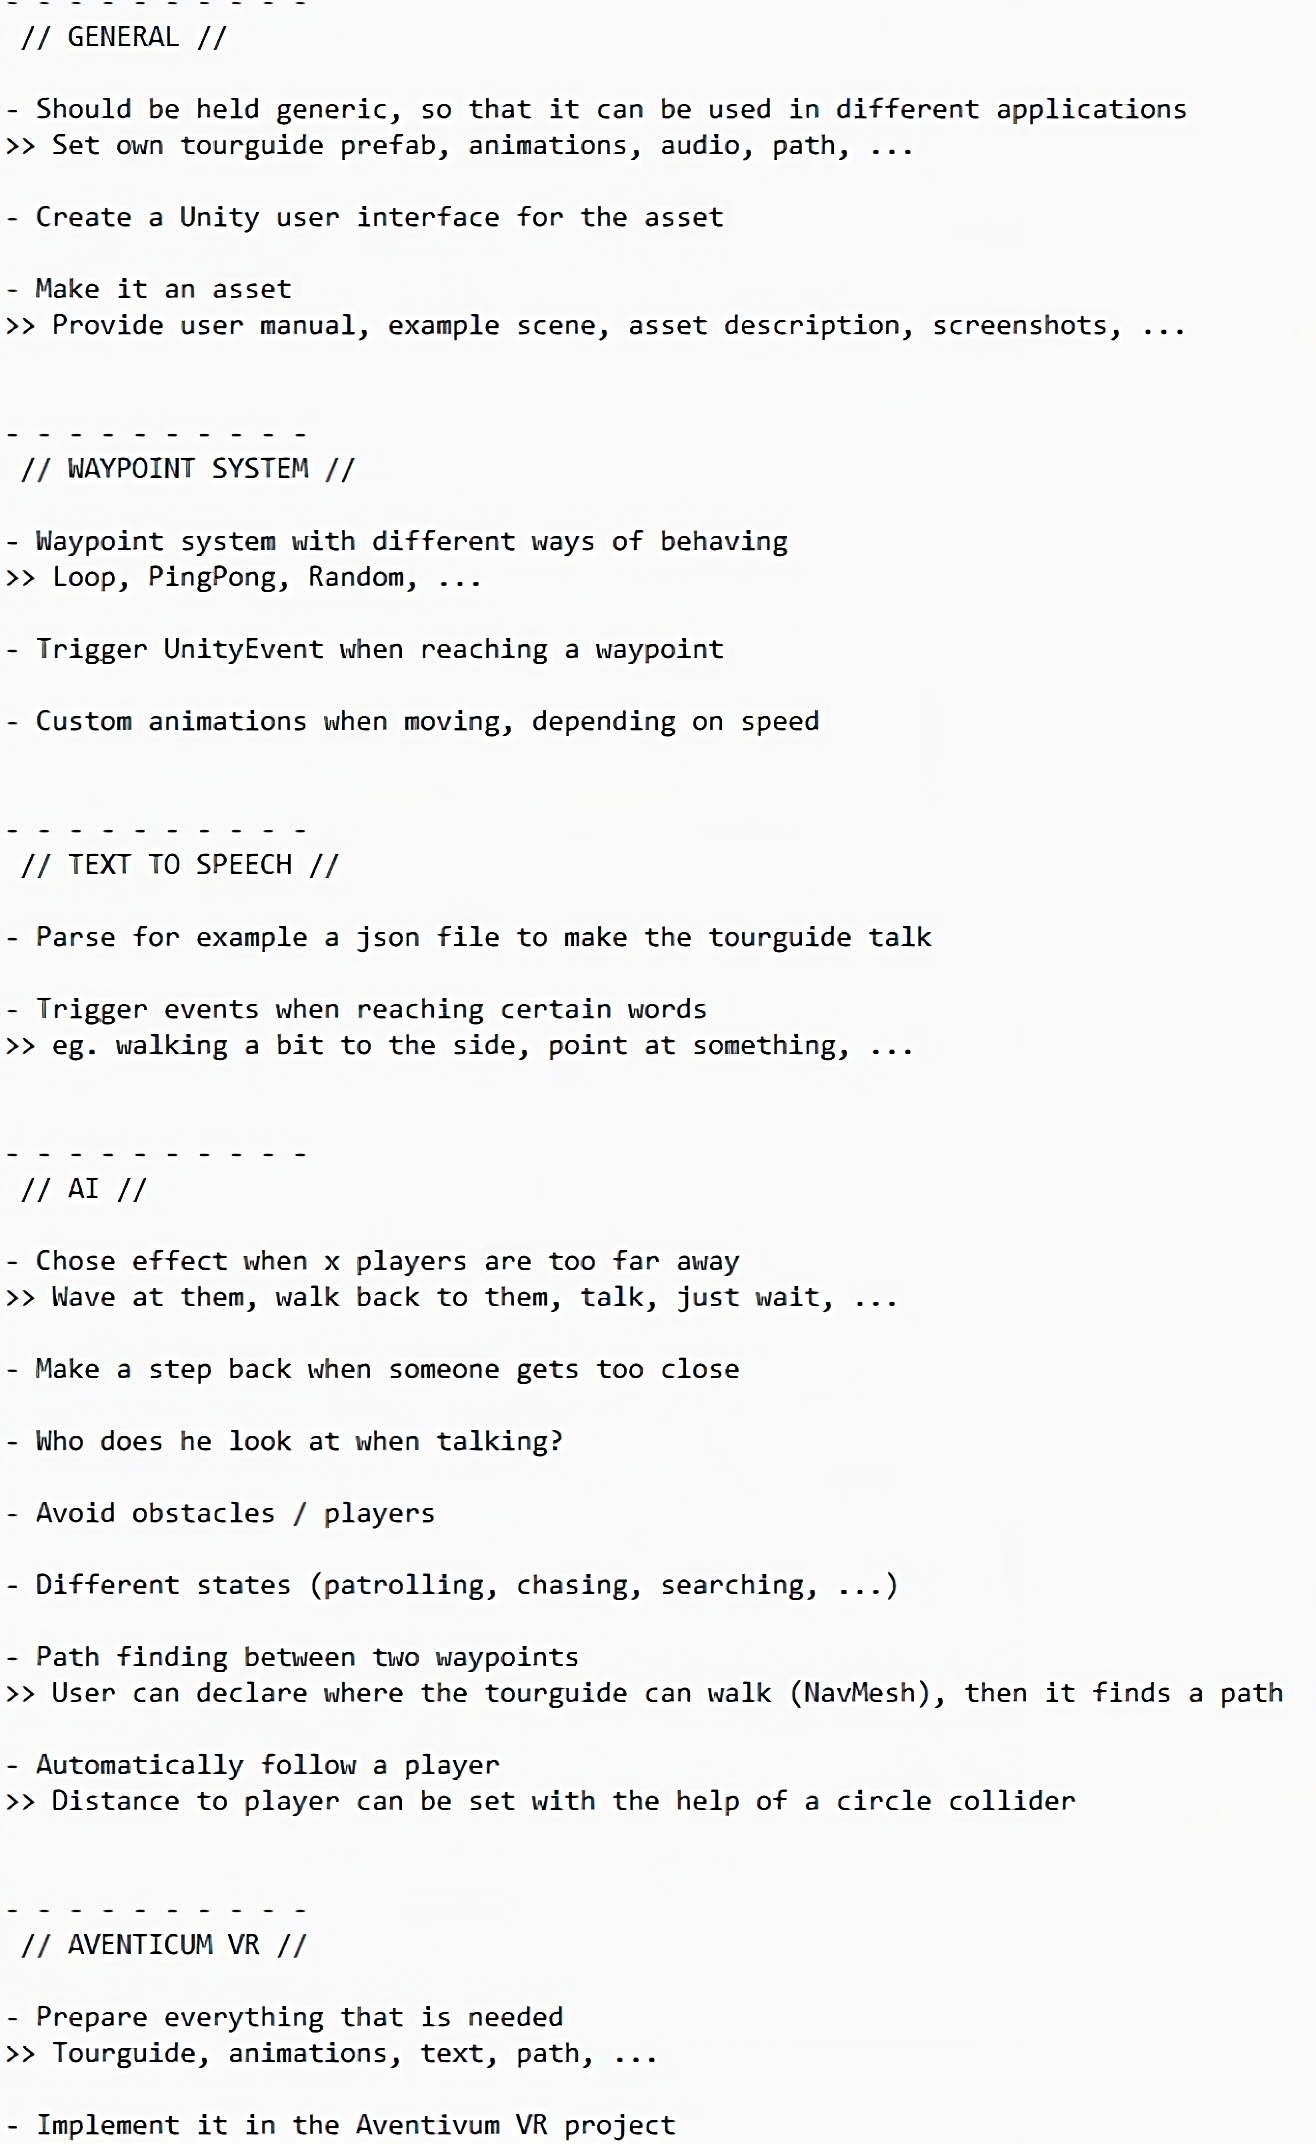
\includegraphics[scale=0.205]{images/bot_controller_idea.png}
	\caption{First Ideas}
	\label{fig:bot_controller_idea}
\end{figure}

Figure \ref{fig:bot_controller_idea} shows the parts into which the project was divided. In the Unity editor, the user could add this asset as a component to the unit they wanted this tool to control. This component could then be edited in the inspector window. The options available for configuring it would be as shown in the figure \ref{fig:bot_controller_idea}. To achieve this goal, the component would have to be created using the Unity editor scripting by deriving from the Editor class. This class provides all the functionality needed to customise the functionality and appearance of the inspector.

\begin{figure}[H]
	\centering
		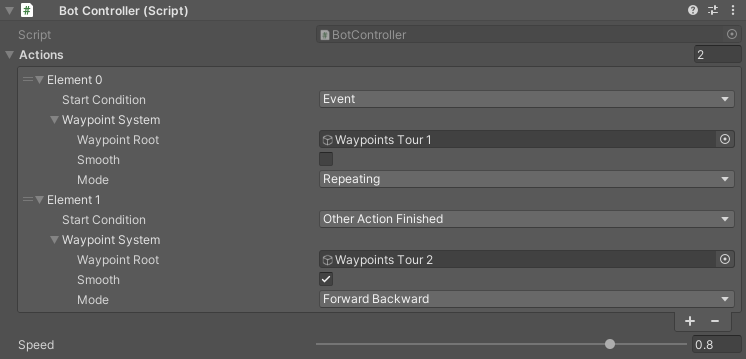
\includegraphics[scale=0.6]{images/bot_controller_gui.png}
	\caption{Example of the GUI in Unity}
	\label{fig:bot_controller_gui}
\end{figure}

This is an example of what an interface created with the Editor class might look like. It's a good visualisation of what part of this tool might look like when it's finished. A new action can be created by clicking on the "+" icon at the bottom right. How exactly the action is triggered can be selected from the "Start Condition" drop down. Once executed, the action would cause the GameObject to which the script is attached to follow the specified waypoints assigned in the "Waypoint Root" field. Once the whole asset was finished, it would have more functionality than just a waypoint system, and would therefore become much more complex.

\begin{figure}[H]
  \centering
  \begin{minipage}{0.45\textwidth}
    \centering
    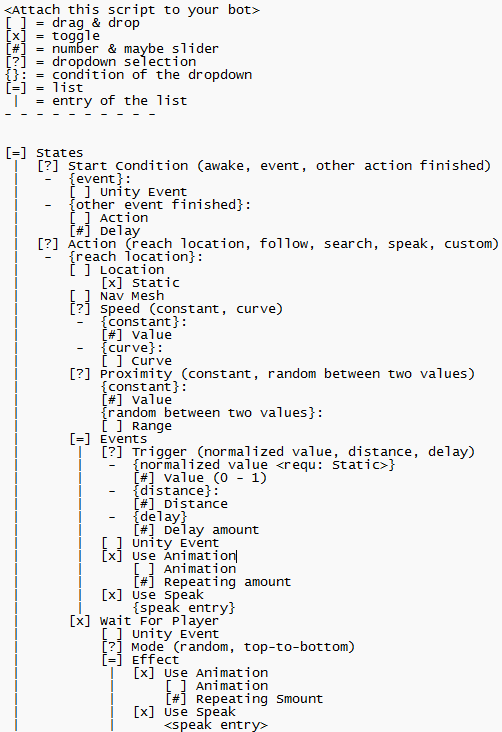
\includegraphics[scale=0.55]{images/bot_contoller_features_1.png}
    \caption{Features page 1}
    \label{fig:bot_contoller_features_1}
  \end{minipage}
  \hfill
  \begin{minipage}{0.45\textwidth}
    \centering
    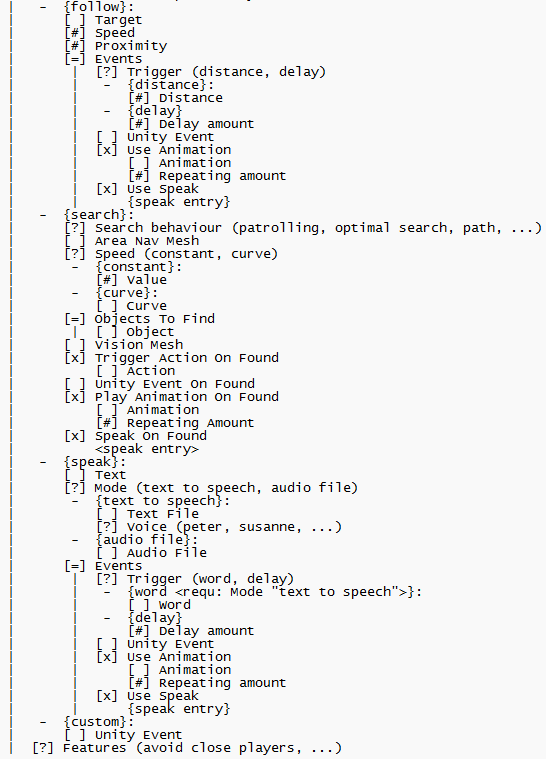
\includegraphics[scale=0.55]{images/bot_contoller_features_2.png}
    \caption{Features page 2}
    \label{fig:bot_contoller_features_2}
  \end{minipage}
  \caption{Features}
  \label{fig:bot_contoller_features}
\end{figure}

This is a sketch of what it might look like with all the features planned so far. At the top is a legend explaining what the symbols mean, and below is a hierarchical structure that allows the user to change the behaviour of this component.

It's a bit hard to understand at first, so here's an explanation of how it works:

The whole system works as a state machine, and new states could be added at will. Each state could be associated with a particular type of action, in the example of figure \ref{fig:bot_contoller_features}, the choices would be "reach location", "follow", "search", "speak" or a custom one. Each of these actions could have different variables to customise its behaviour. A "Start Condition" could be selected to define when an action should start. During an action, events could be triggered which could be used by the programmer or alternatively cause a change of state.

With this approach, the developer would have the option of either selecting one of the predefined actions or creating a new one. This could be used to create a behaviour in a relatively short amount of time.

\newpage

\section{Trouble}
\label{sec:projectevolution_trouble}

The problem with this solution is that the whole structure becomes very messy and hard to read as the number of actions grows. The main reason for this is that it becomes hard to see which state leads to which, and because it's a state machine, the number of states and links between them can grow quite quickly. So a graphical approach might help against this problem. If each action were a node in a graph, it would be much easier to see how everything is connected.

\section{Better Approach}
\label{sec:projectevolution_betterapproach}

The next idea was to implement this generic behaviour creator as a sequence graph. Each node represents an action, and each of these nodes can be freely connected to other nodes by an edge. In order for a state change to occur, a particular event must occur on the currently executing node.

\begin{figure}[H]
	\centering
		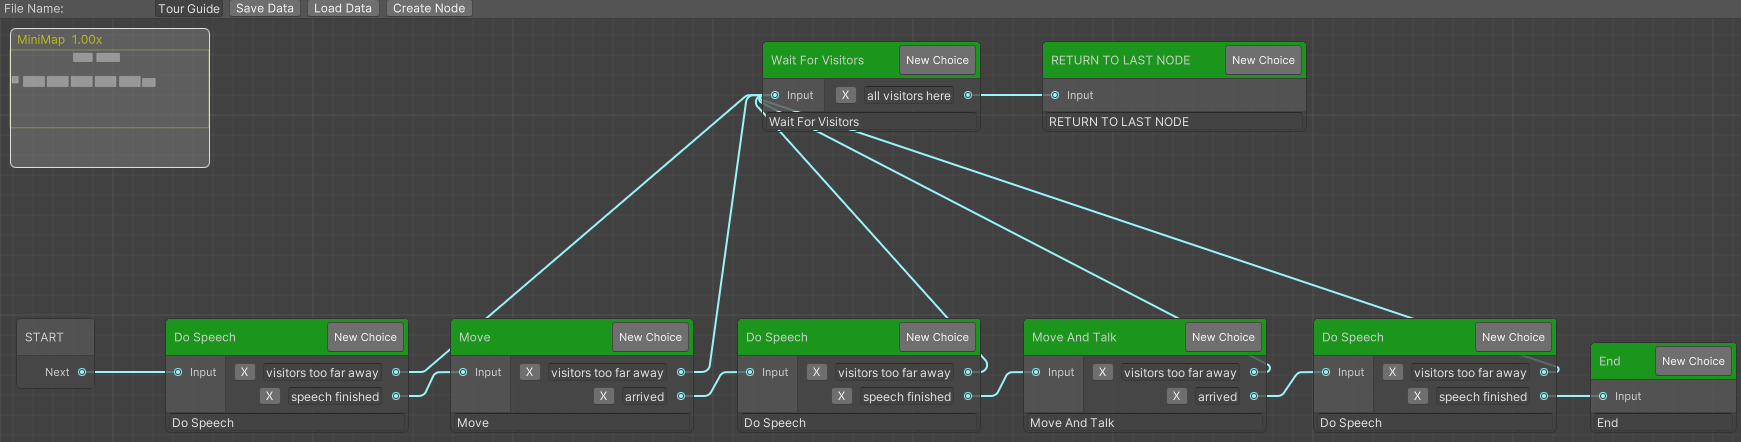
\includegraphics[scale=0.34]{images/sequence_graph_tour_guide.png}
	\caption{Sequence graph example for tour guide}
	\label{fig:sequence_graph_tour_guide}
\end{figure}

This graphic shows a very simple version of what a tour guide system might look like when it's finished. It was implemented to get more familiar with how programming a graphical interface for Unity works, and also to find out its advantages compared to scripting in the editor. Each node represents an action that the agent can perform, and each edge leads to a state change that can be triggered by one of the conditions.


For example, in figure \ref{fig:sequence_graph_tour_guide}, the behaviour would start at the "START" node on the left. It would immediately start executing the first "Do Speech" action, looking for triggers that a visitor is too far away or that the speech is finished. If one of the conditions for a trigger is met, a state change will take place. In the example of a visitor being too far away, the tour guide would go to the node at the top and perform the action "Wait for Visitors". As soon as the visitors are close enough again, the tour guide would continue his speech until the visitors are too far away again or the speech is finished. This behaviour will continue until the "End" node is reached, at which point it will stop.

By using a sequence graph, the whole structure looks more organised and nodes can be freely moved around and connected to other nodes. This makes it easier for the user to create the right behaviour for their application. The conditions for triggering the next action can also be programmed separately, allowing the same trigger to be used in multiple nodes, reducing the amount of scripting required.

\section{Why It Fails}
\label{sec:projectevolution_whyitfails}

Essentially, the whole structure is just a finite state machine (FSM), optimised mainly for implementing a tour guide. There are several problems with such an approach. One is that once there are many edges, it becomes difficult to understand which edge leads to which state.

\begin{figure}[H]
	\centering
		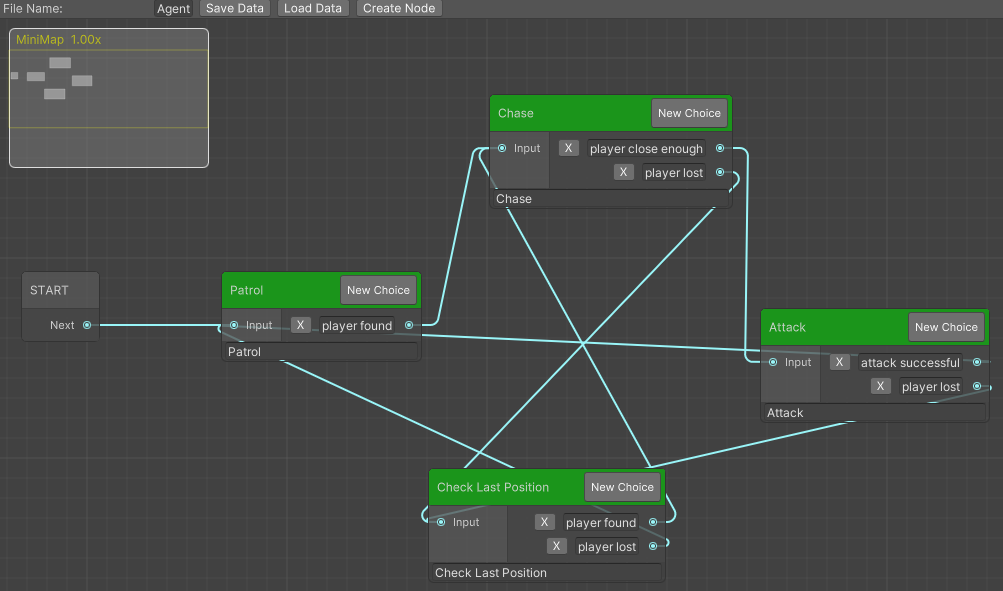
\includegraphics[scale=0.45]{images/sequence_graph_agent.png}
	\caption{Sequence graph example for an agent}
	\label{fig:sequence_graph_agent}
\end{figure}

This screenshot shows the behaviour of an agent patrolling the area around him. If it finds a player, it will try to attack them, and if it loses the player, it will check their last seen position. This is a fairly simple behaviour with only four states and eight edges, but it already looks very messy and hard to follow, and this problem will only get worse as it grows in size and complexity.

Another problem is loops and repeating sequences in general. As you can see in figure \ref{fig:sequence_graph_agent}, there are several loops built in, one of which is "Patrol" - "Chase" - "Check Last Position". There is no way to get rid of the loops in this example, and they are usually the cause of the disarray. As the name suggests, sequence graphs are excellent for sequential behaviour, like a dialogue graph or a shader graph, but struggle with an organised look when it comes to repeating behaviour.

Since the behaviour of a tour guide is sequential, a sequence graph would work well for it. However, this asset should become a tool that is useful for other types of behaviour as well, and many Non-Player Characters NPCs in games are based on repetitive behaviour. Therefore, a solution is needed that also supports loops, while retaining the flexibility of a graph.

In addition, as the complexity of a behaviour increases, it would be helpful if certain parts of the graph could be collapsed so that only the core parts remain visible. Unfortunately, this isn't possible in a graph that can contain loops, because any state can be connected to anywhere, and there is no tree-like structure that would allow this.

The FSMs could be organised into a hierarchical structure, by completely extracting certain parts of the graph, to make them easier to read. But this would still not solve the problem that they would become unmanageable once they reach a certain complexity.

All these problems combined together explain why this approach isn't optimal, however, a behaviour tree looks like it solves all of these issues.
\chapter{Behaviour trees}
\label{chap:behaviourtrees}
\section{What Are Behaviour Trees}
\label{sec:behaviourtrees_whatarebehaviourtrees}

Behaviour trees (BTs) are often used in game development to create the behaviour of autonomous agents. They are used to switch between a finite set of tasks and are very modular, making it easy to iterate through different examples. BTs have become popular because they are very good at creating complex behaviours from simple individual tasks. A BT needs different types of nodes to work. \cite{BehaviourTrees}

Depending on the implementation, this may vary slightly, but in general there are four types:

\begin{tabular}{ll}
Composite: & Defines the base rule for how the branch is executed. \cr
Decorator: & Able to modify the return value of a node. \cr
Action: & Contains the logic to be executed when it's invoked. \cr
Conditional: & Used to make Boolean decisions based on the defined condition.
\end{tabular}

Composite nodes are responsible for deciding which action node to call and execute next. It's decision is based on the return value of its children. A node can return the status Running, Success or Failure.

\begin{figure}[H]
	\centering
		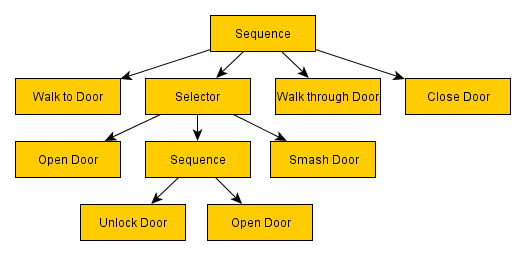
\includegraphics[scale=0.5]{images/behvaiour_tree_example_door.png}
	\caption{Example of a behaviour tree \cite{BehaviourTrees}}
	\label{fig:behvaiour_tree_example_door}
\end{figure}

This is an example of an agent trying to go through a door and then close it. The tree is executed from top to bottom and from left to right. The first node in this example is a composite node, the "Sequence". It starts by executing the leftmost child node and waits for it to finish, in other words, it waits for the "Walk to Door" action to return either success or failure. The Sequence composition works much like an AND operation. It must have all its children return Success for it to also return Success. If only one child returns Failure, it will immediately return Failure. After the first child returns Success, in this example the "Walk to Door" action, it will sequentially execute the next task, which would be the "Selector" node.

The Selector is the opposite of the Sequence node and works like an OR operation. This means that if the first child returns Success, it will also return Success, otherwise it will return Failure. Once the "Selector" node is executed, the agent tries to open the door, and if this fails, the next node is executed, which is another Sequence node. In this sub-tree, the agent will try to unlock the door first and then open it, and if either of these fails, the Smash Door action will be called.

After the door has been opened - by whatever means - the agent will then walk through the door and finally close it. This example consists only of composite and action nodes.

An action node defines the logic that happens when the node is executed. There are also other types of nodes, such as the parallel composite, which allows the actions to be executed in parallel.

Decorators can be used, for example, to invert the return value of an action, or to make it repeat until it returns success or failure.

\section{Example Implementations}
\label{sec:projectevolution_exampleimplementations}

To learn more about behaviour trees, some sample scenes have been created using Unity. For this example, the Behaviour Designer asset from the Unity Asset Store was used, which provides a very intuitive implementation of a behaviour tree.

\subsection{Agent Scene From Advanced 3D Applications}
\label{subsec:projectevolution_exampleimplementations_agentscenefromadvanced3dapplications}

\begin{figure}[H]
    \centering
    \begin{minipage}{0.49\textwidth}
        \centering
        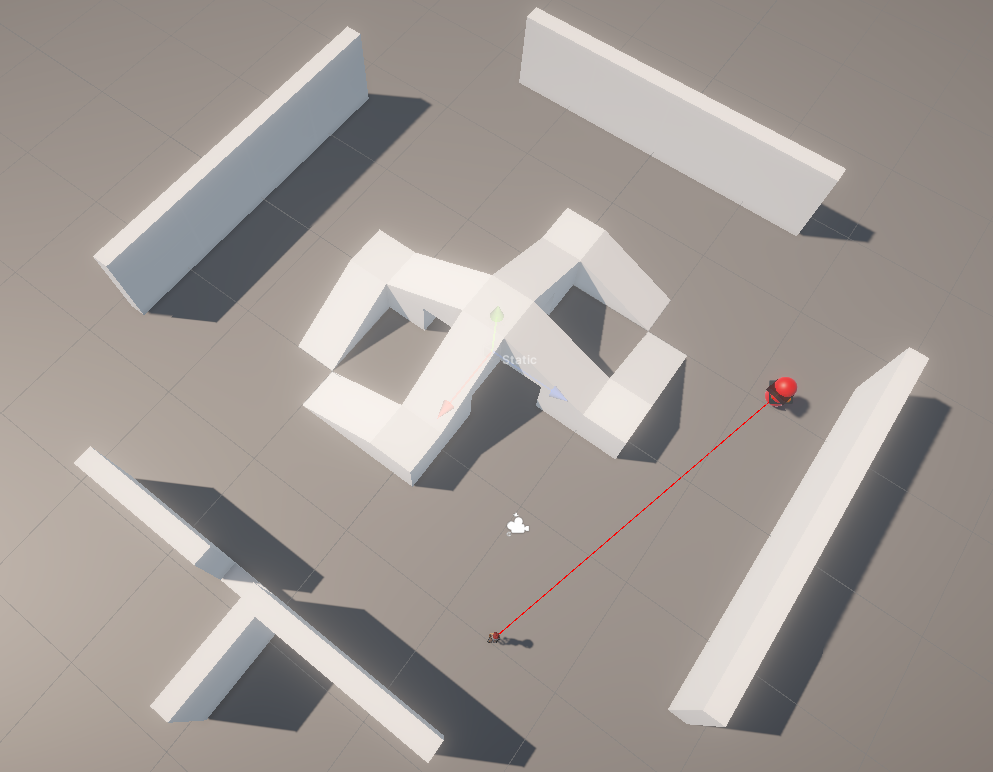
\includegraphics[scale=0.3]{images/behaviour_tree_scene_agent.png}
        \caption{Scene in Unity with the agent}
        \label{fig:behaviour_tree_scene_agent}
    \end{minipage}
    \begin{minipage}{0.49\textwidth}
        \centering
        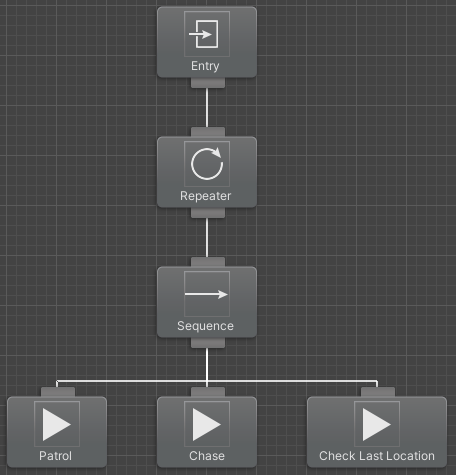
\includegraphics[scale=0.49]{images/behaviour_tree_agent.png}
        \caption{Behaviour tree for the agent}
        \label{fig:behaviour_tree_agent}
    \end{minipage}
\end{figure}


The first example shows an agent who chases the player, called Sintel, as soon as it sees her. The agent will simply patrol the area around him until he sees her, and then start chasing her. Once the line of sight is broken, the agent will check her last location and then resume patrolling.

The BT for this example looks very simple, there is just a repeater node at the top, which will act as an endless loop for the agent. The following Sequence node will therefore continue to execute the three Action nodes from left to right until one of them fails, at which point it will restart with the "Patrol" state.

\subsection{Tour Guide}
\label{subsec:projectevolution_exampleimplementations_tourguide}

\begin{figure}[H]
	\centering
		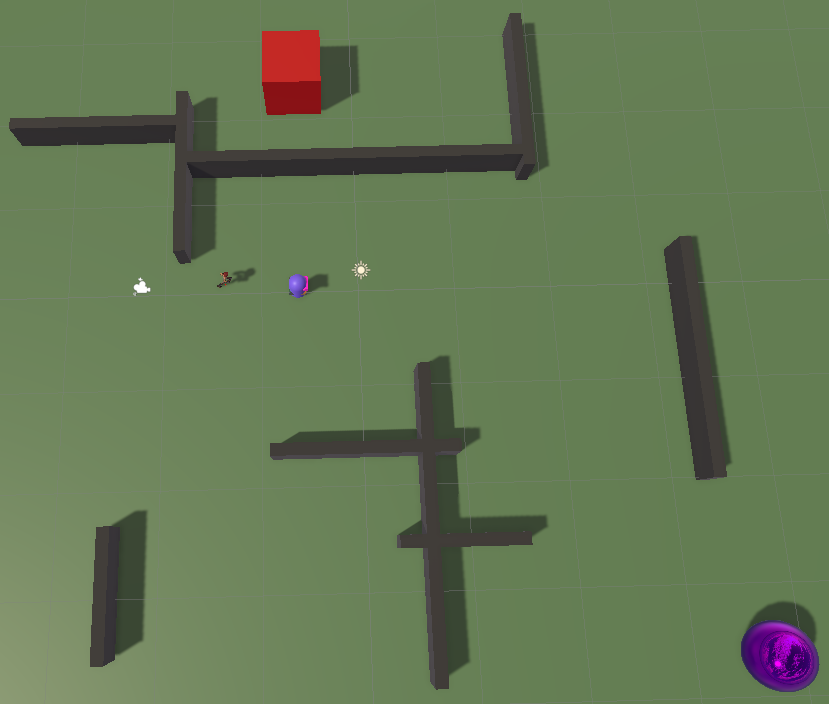
\includegraphics[scale=0.35]{images/behaviour_tree_scene_tour_guide.png}
	\caption{Scene in Unity with the tour guide}
	\label{fig:behaviour_tree_scene_tour_guide}
\end{figure}

As the original idea was to make a tool for a tour guide, the second example shows a tour guide implementation using a BT. The sphere and the cube are placeholders for an object that the tour guide can show to the visitor. The tour guide will first walk to the sphere, say some text there, then walk to the cube while also talking on the way there, and finally talk about the cube. Whenever the visitor is too far away, he will stop and wait for them.

\begin{figure}[H]
	\centering
		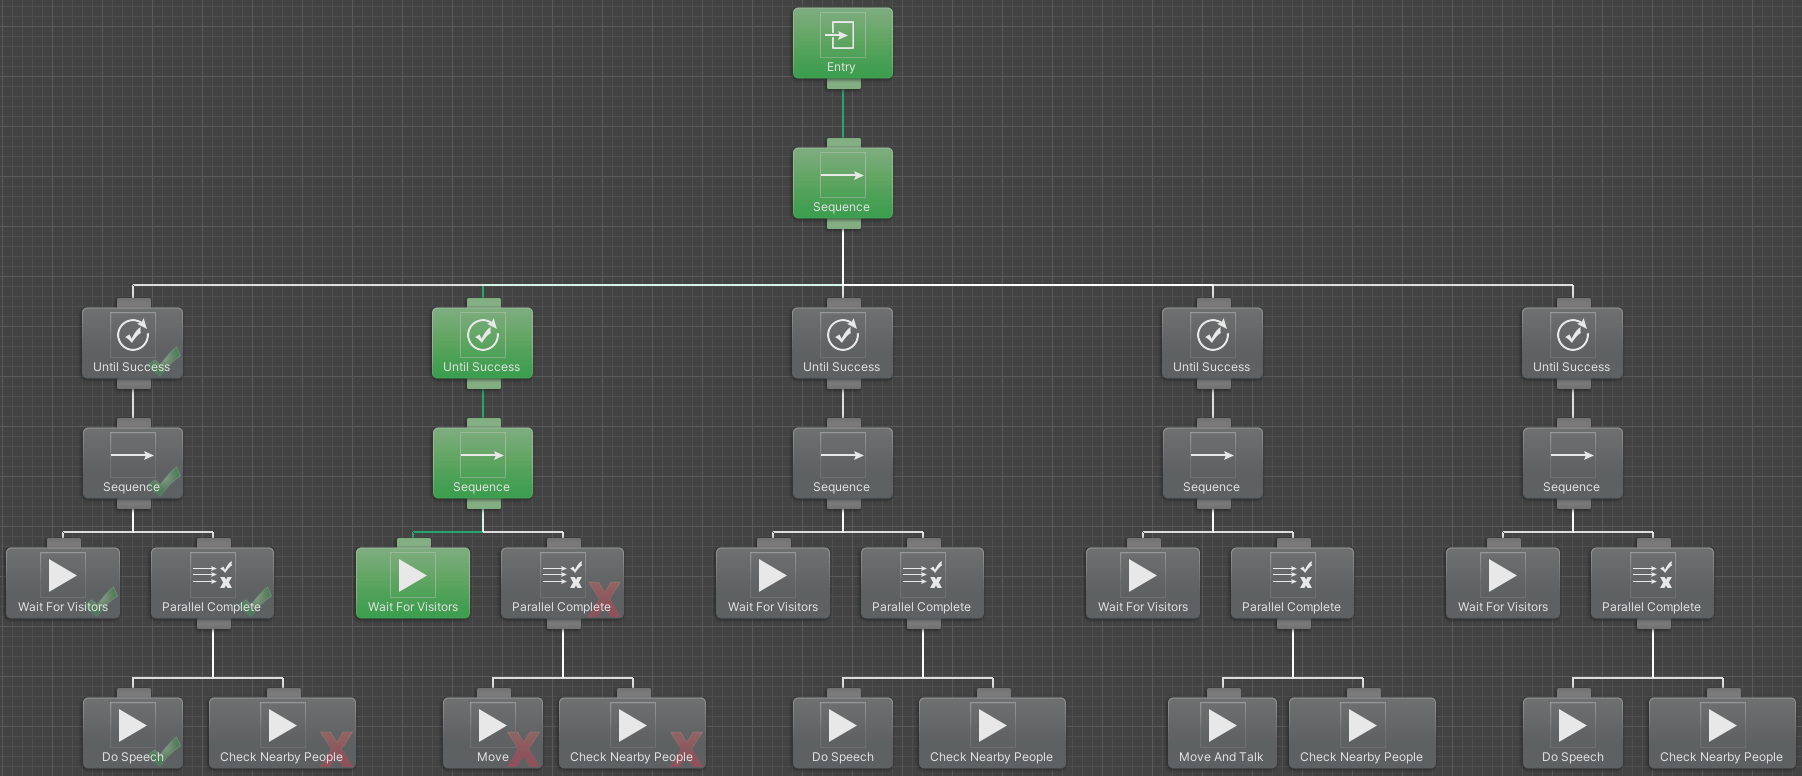
\includegraphics[scale=0.328]{images/behaviour_tree_tour_guide.png}
	\caption{Behaviour tree for the tour guide}
	\label{fig:behaviour_tree_tour_guide}
\end{figure}

This screenshot was taken while the simulation was running, so the current state (in green), the successful states and the failed states of the BT are marked. The first element is a sequence, followed by five subtrees. Each sub-tree is built in the same way: It waits until the visitor is close enough, then does something until the visitor is too far away, at which point it waits again. The bottom left node of each sub-tree tells you what behaviour it will perform.

\section{Strengths}
\label{sec:projectevolution_strengths}

A behaviour tree can be expanded to many hundreds of nodes or even more, and sub-trees can be collapsed for a better overview, making it a very good option for defining simple and complex behaviours.

BTs are also very generic because their action nodes are independent of the overall structure and can be implemented according to the needs of the scenario. Once an action node is implemented, it can be reused over and over again without having to write the same code twice.

In addition to that, BTs are also very intuitive once the basic concept is clear. They can be read and understood by someone who doesn't know much about programming. They're also easy to test and debug, given a good implementation.

\section{Weaknesses}
\label{sec:projectevolution_weaknesses}

Although the behaviour tree is a very powerful concept, it is not perfect for every situation. It starts to have problems when it comes to creating more complex NPCs that can react instantly to any kind of situation, even if some information is missing. BTs are definitely more organised than FSMs and can handle complex behaviour better, but they still suffer from the problem that every possible decision has to be pre-defined manually. Not having to specify the decision for every case would save a lot of time for more intelligent behaviours, and could also make them look more realistic if they were able to decide on their own.

Also, BTs can become expensive as they grow larger, because the cost of evaluation depends heavily on the number of nodes. This is because, naively, the whole tree is evaluated every tick to recompute all the conditions, just to check that the current behaviour is still valid. This can be compensated for by a clever implementation, but it will make the implementation more difficult.

\chapter{Utility AI}
\label{chap:utilityai}

\section{Idea Of Utility AI}
\label{sec:utilityai_ideaofutilityai}

The main goal of utility AI is to give NPCs more dynamic behaviour while keeping everything simple to read and understand. The general idea has been around for a while, but has been given a remarkable push by Dave Mark, president and lead designer of Intrinsic Algorithm LLC. Utility AI is about giving NPCs some information and possible actions, and then letting them decide for themselves what is the best action to take given the current circumstances. The goal is to make the AI feel alive and responsive by doing a very simplified version of what humans do when making a decision: Evaluate the circumstances and choose the best resulting action. \cite{UtilityAiFunctionality}

The way utility AI works is that the NPC has a predefined set of possible states, and each time it decides what to do next, it evaluates all the states based on their associated considerations. A consideration is just some information about the environment. The state with the highest score is then executed next, causing the NPC to take action.

\section{Terminology}
\label{sec:utilityai_terminology}

To avoid confusion between the different aspects of utility AI, the following terminology is used in this paper:

\begin{tabular}{lp{12cm}}
State Set: & A simple container of states to help organise the states and allow runtime changes to state sets. \cr
State: & A state that the NPC can be in. While in a state, the NPC performs a task as defined in the state's behaviour tree. It has two other components: preconditions and evaluators, which are responsible for calculating the state's score. \cr
Precondition: & Each state can have any number of preconditions. If a precondition is not met, the state will not be selected, regardless of its score. \cr
Evaluator: & Each consideration can optionally be associated with an evaluator, which will then score it using an adjustable curve. \cr
Consideration: & The NPC's knowledge of his needs and his environment. Its value can change over time and is used as input for evaluating states. \cr
Weight: & Evaluators and actions each have their own weight. It can be used to change the NPC's overall preferences. \cr
Score: & The utility NPC's scoring system, used to decide the best state.
\end{tabular}

\section{How It Works}
\label{sec:utilityai_howitworks}
\subsection{General Principle}
\label{subsec:utilityai_howitworks_generalprinciple}

A state set contains several states, which are iterated through to evaluate the score of each and then select the one with the highest score.

\begin{figure}[H]
	\centering
		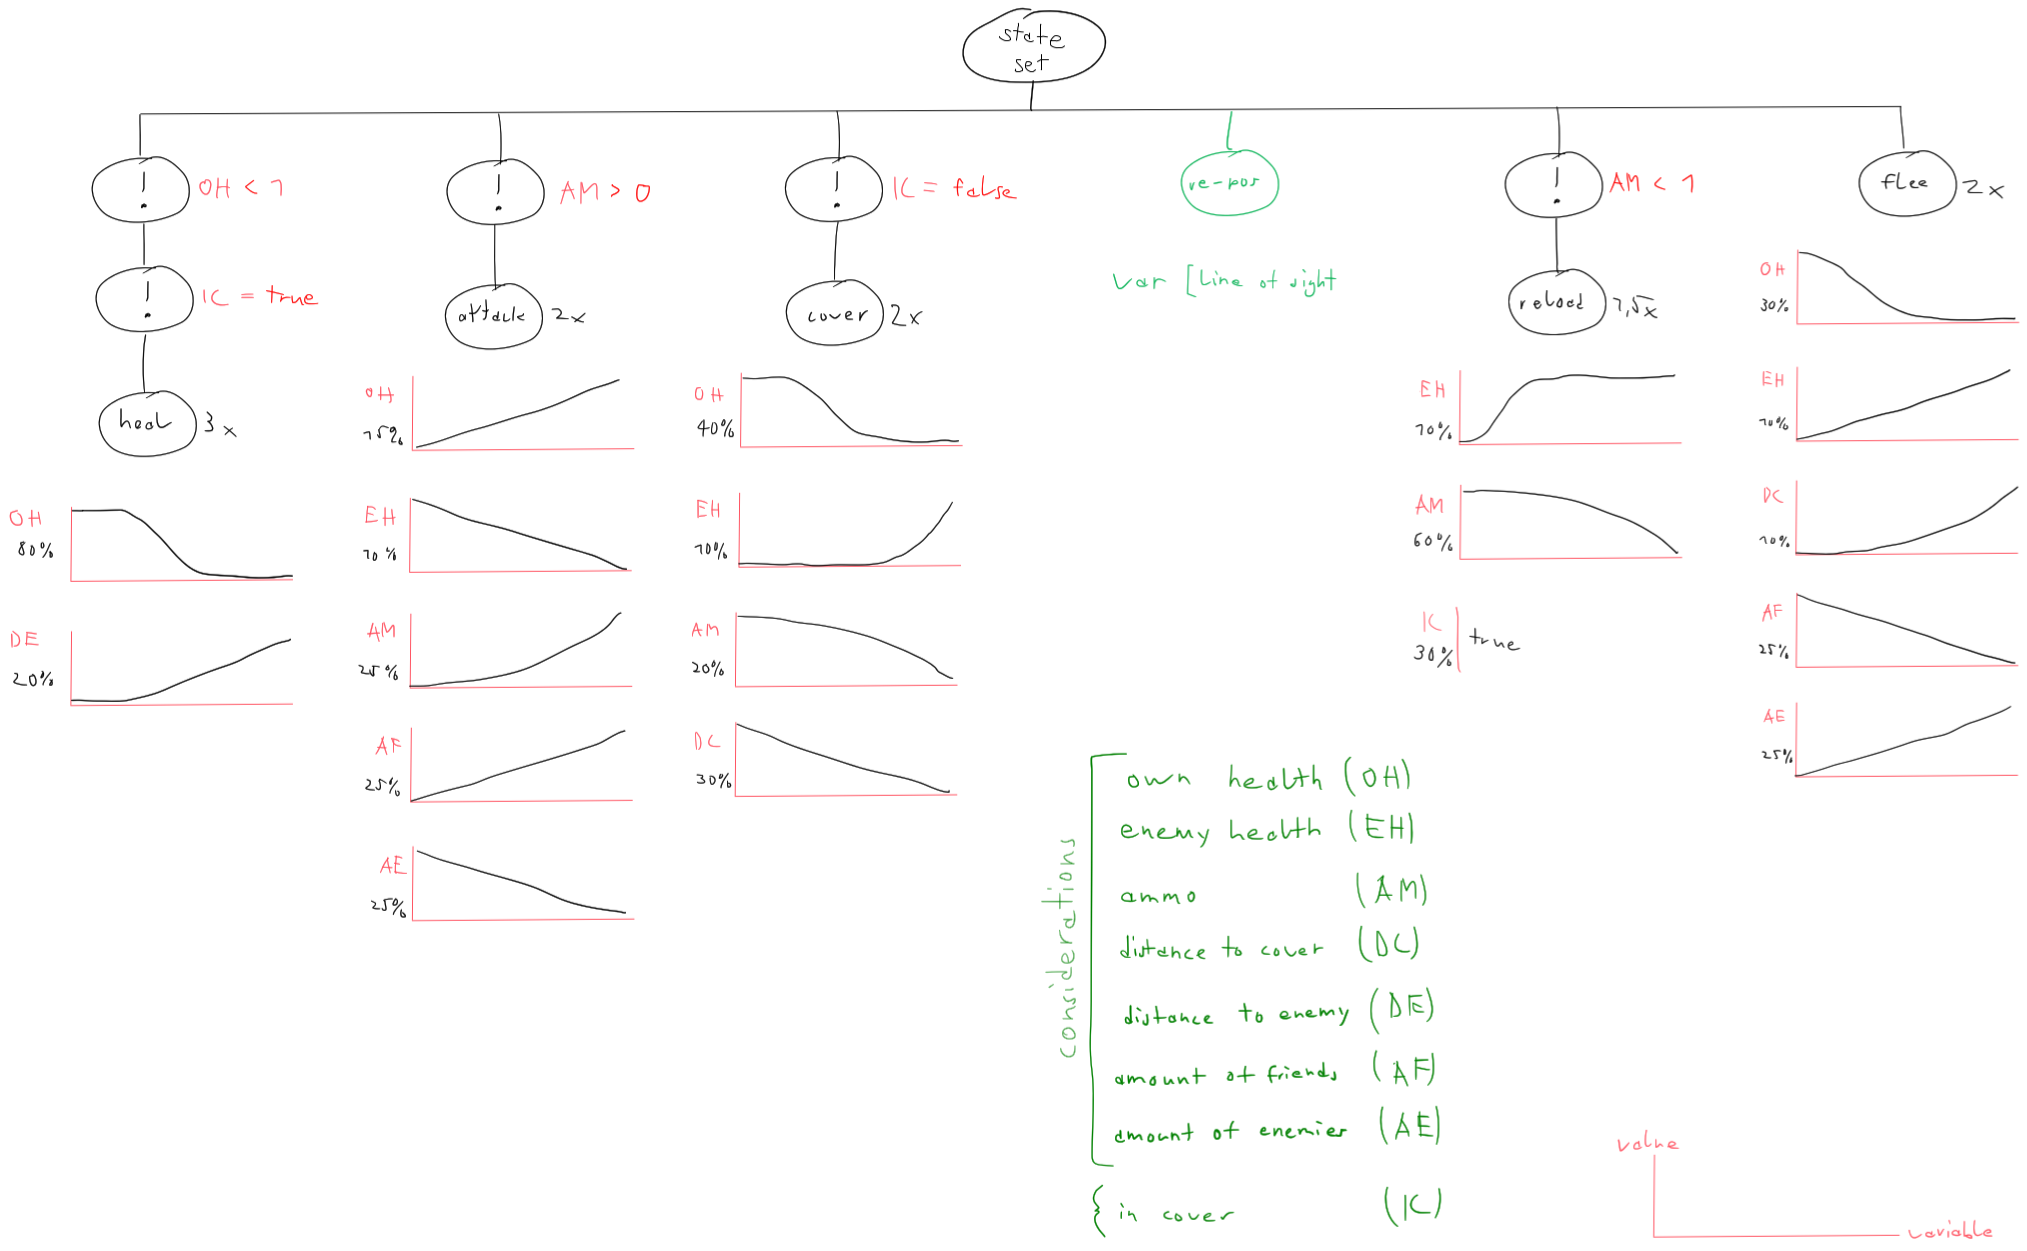
\includegraphics[scale=0.29]{images/utility_ai_sketch_defending_ai.png}
	\caption{Sketch of a defending NPC, using utility AI}
	\label{fig:utility_ai_sketch_defending_ai}
\end{figure}

This is the structure of an example scenario for a utility AI. It shows the behaviour of an agent trying to defend its territory against intruders.

As an example, below the "heal" state on the left are two curves representing the evaluators. For the first curve, the OH (own health) consideration is evaluated and scored from 0 to 1 based on the function of the curve with own health as the input parameter. The score is then multiplied by its weight, in this case 0.8. The same is done for the DE (distance to enemy) consideration.

All the scores from the evaluators will return a sum less than 1. This sum is then multiplied by the weight of the state, in the case of "heal" it would be multiplied by three.

A state will only be considered if each condition is met. In the "heal" example, the OH (own health) consideration must be less than 1 and the agent must be in cover, otherwise the state will be ignored.

The same procedure is then performed for each state that is in the state set.

\newpage

\subsection{Calculation Of The Score}
\label{subsec:utilityai_howitworks_calculationofthescore}

Dave Mark used a different formula to the one used in this paper. In his formula, all the scores from the evaluators are multiplied together, which then gives the total score. Since multiplying decimals will continuously make them smaller, he applies an averaging scheme to each action after it has received its score to compensate for this.

\begin{equation}
ActionScore = Score + \left(1 - Score\right) \cdot \left(1 - \frac{1}{TotalConsiderations}\right) \cdot Score
\end{equation}

This formula works for calculating the average score, but there is still a problem that might want to be avoided for certain scenarios. If one of the considerations scores 0 or close to 0, the final score will also be 0 or close to 0, no matter how well the other considerations score. \cite{UtilityAiTalk}

In the figure \ref{fig:utility_ai_sketch_defending_ai_with_values}, for example, if the evaluator for EH (enemy health) returns 0, the agent would never reload, no matter how little ammo was left in its weapon. Obviously this isn't the desired behaviour, unless a consideration is not allowed to be 0 for the state to work, but in this case a precondition could be used.

To overcome this problem, all the scores are instead added together and then divided by the total number of scores used. This approach is also simpler because it doesn't require an averaging scheme, so it's more intuitive to work with.

Up to here, the scores have simply been averaged without any weights. In order to add weight to the formula, the most straightforward solution is to give each evaluator a percentage representing its importance. Each score is then multiplied by this percentage before being added to the total score. A visualisation of this idea can be seen in the figure \ref{fig:utility_ai_sketch_defending_ai_with_values}.

Calculating the weight in this way introduces a new problem. If a new evaluator is added later, all the previous weights must be adjusted because the total percentage must be 100\%.

To address this issue, the weight of each evaluator is not set as a percentage, but as a decimal between 0 and 1. The corresponding percentage is then calculated in the background by dividing its weight by the sum of all weights. This way the weight of each consideration doesn't need to be changed when a new weight is added. The following equation is used to obtain the total score of a state:

\begin{equation}
TotalScore = StateWeight \cdot (BaseScore + \sum_{i=1}^{n} \left( Score_i \cdot \frac{EvalWeight_i}{TotalEvalWeights} \right))
\end{equation}

where \textit{n} is a list of all evaluators, and \textit{TotalEvalWeights} the sum of all weights from the evaluators of the state. The \textit{StateWeight} represents the weight that can be manually adjusted to change the overall importance of the state, as seen in the example figure \ref{fig:utility_ai_sketch_defending_ai_with_values} to the right of each state.

Each state also has a custom \textit{BaseScore} which is simply added before being multiplied by the \textit{StateWeight}. There is also the option to clamp the \textit{TotalScore} between two custom defined values.

A further problem arises when two states have almost identical scores, which can lead to the agent constantly switching between them. To prevent this, the current action has a bonus factor that can be set individually. This bonus factor is multiplied by the score of the state if it is the state currently being executed. This factor should be greater than one, for example 1.5, to give the current state a higher rating.

\subsection{Example Scenario}
\label{subsec:utilityai_howitworks_generalprinciple}

\begin{figure}[H]
    \centering
    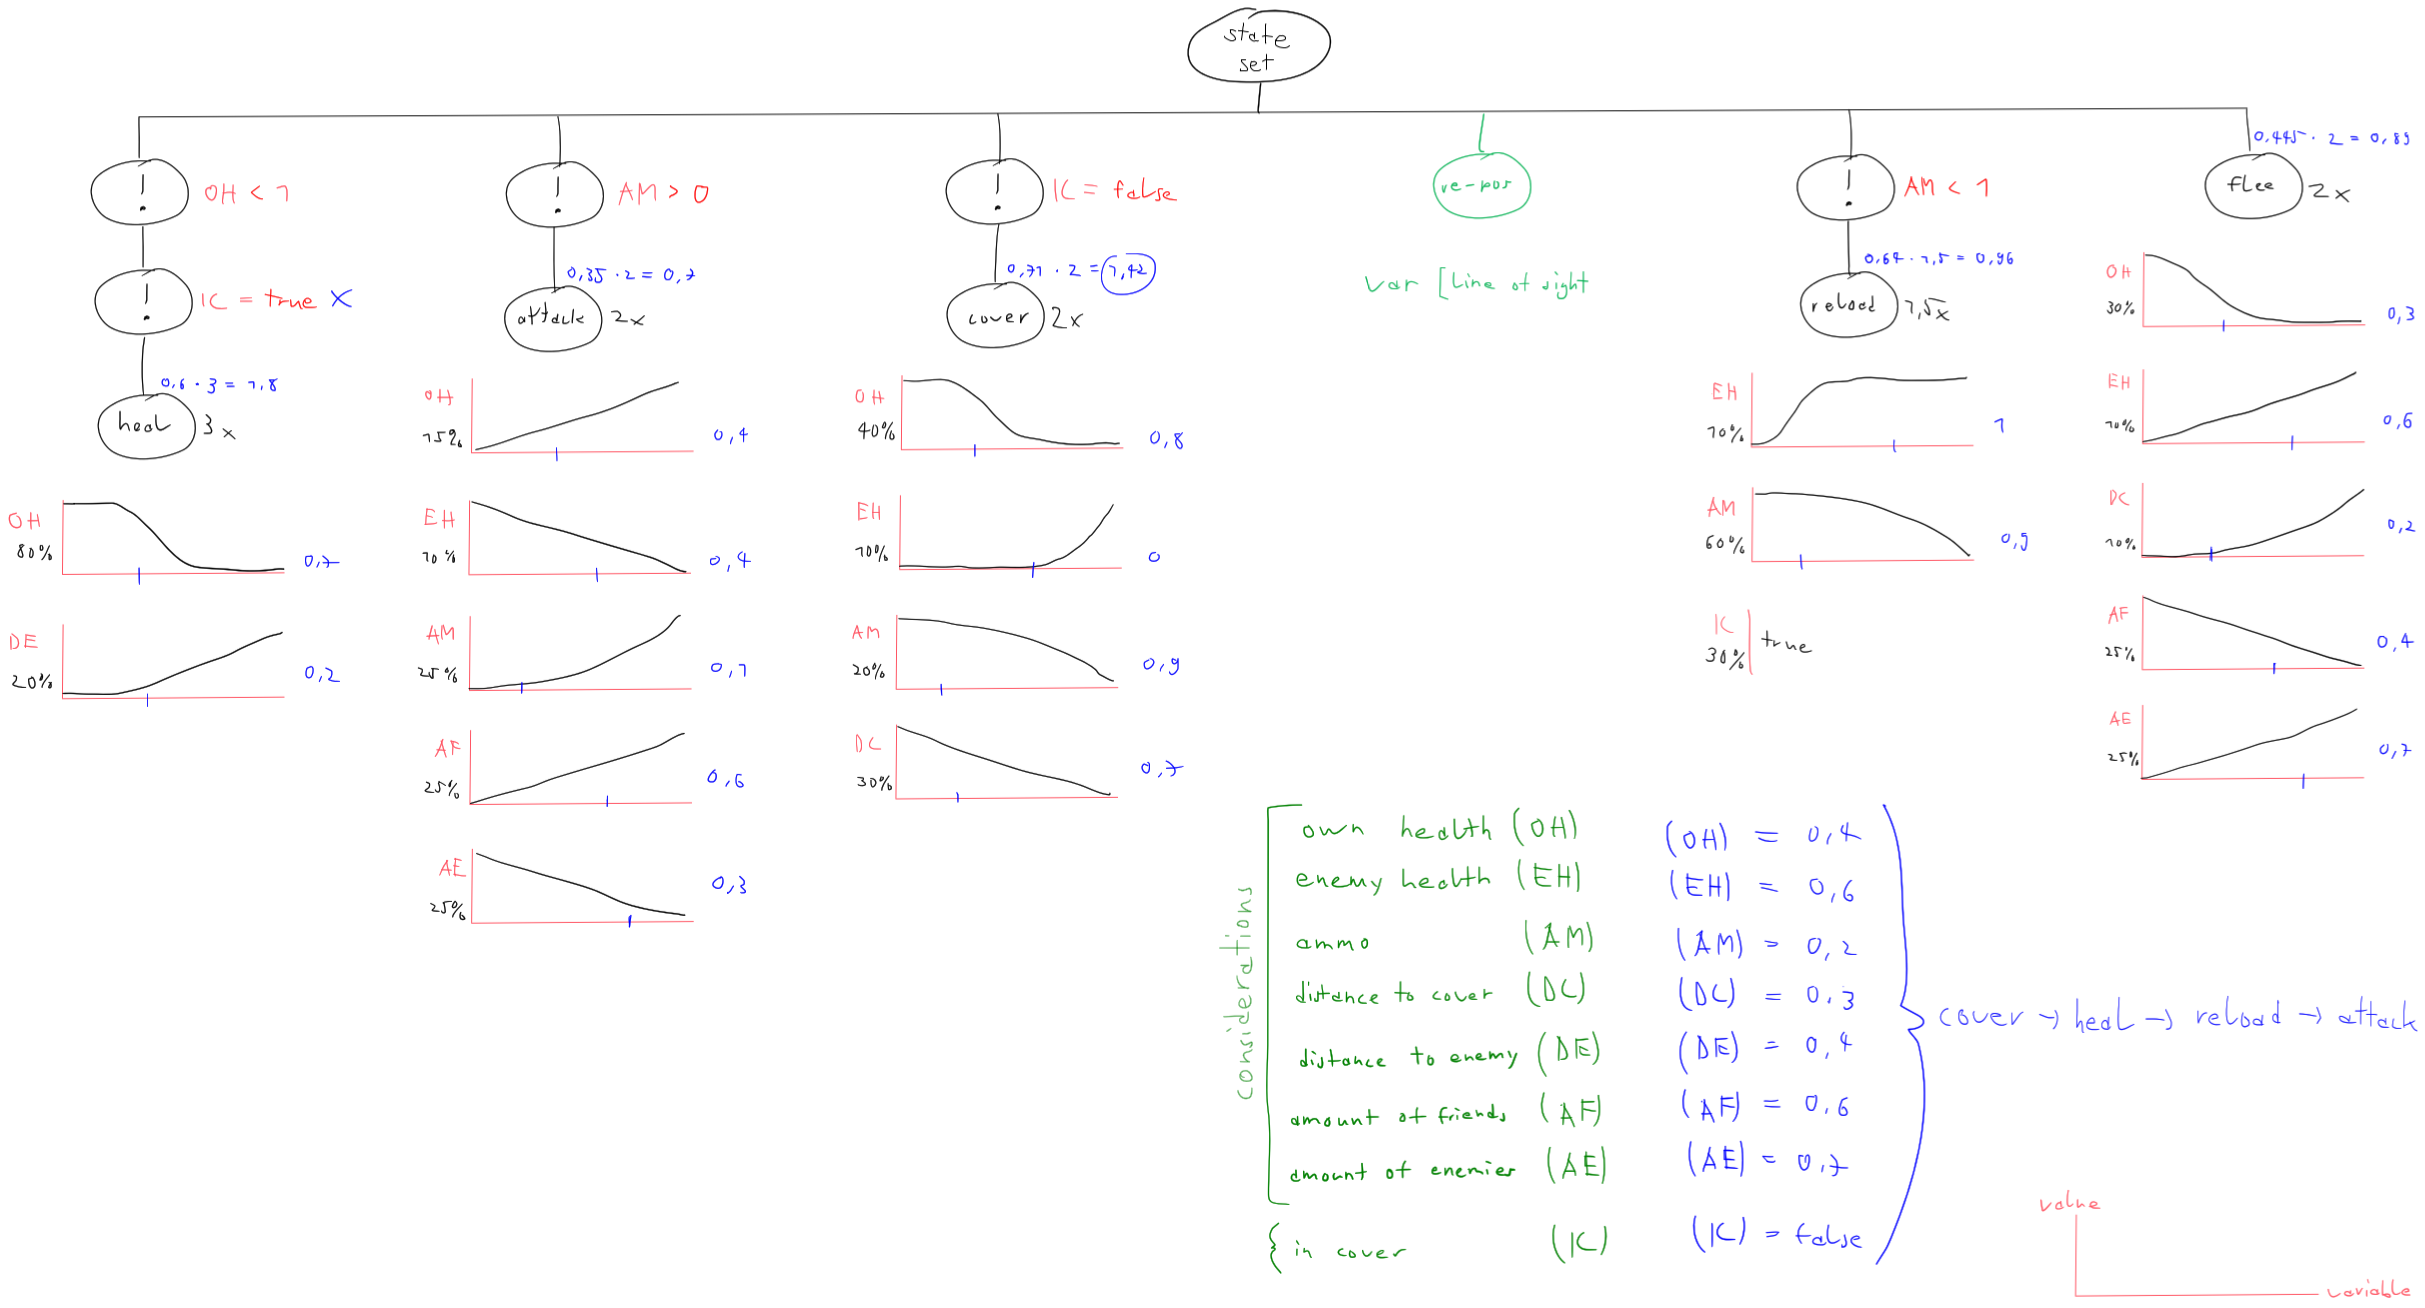
\includegraphics[scale=0.345, angle=90]{images/utility_ai_sketch_defending_ai_with_values.png}
    \caption{Sketch of a defending NPC, using utility AI and with example values}
    \label{fig:utility_ai_sketch_defending_ai_with_values}
\end{figure}

To better illustrate the idea of utility AI evaluation, some sample values have been chosen for all considerations to represent a possible state of the game.

Next to each evaluator is a number in blue, which represents the resulting value of the curve, given its respective consideration. The sum of these, together with the sum multiplied by the weight of the state, can be found next to each state.

In this particular scenario, the "heal" state has the highest score, but because one of its preconditions is not met, it is ignored. "cover" has the second highest score, and since all of its preconditions are met, it is selected as the next state.

Once the agent has reached cover, the next state to be executed is "heal", as it now fulfils all its requirements and still has the highest score.

After healing, the agent will most likely reload its weapon and then start attacking. The order of states may change as the game progresses. For example, if the agent gets badly injured while reloading, it will be less likely to attack. It all depends on the current state of reasoning.

\section{Example Implementations}
\label{sec:utilityai_exampleimplementations}
\subsection{Main Goal Of The Implementations}
\label{subsec:utilityai_realization_maingoaloftheimplementations}

Because the idea of utility AI isn't very well known, and also because the implementation used here differs in some ways from Dave Mark's, the concept needs to be tested first. To do this, a proof of concept was created in the Unity game engine, as it is one of the most popular game engines and supports the creation of new frameworks very well.

These quick implementations ar for proof-of-concept purposes only, and are not optimised for use in real projects. The easiest way to prove that utility AI works as expected is to create a simple framework for utility AI, and then create some example scenes that show its application. This way it is easy to see if utility AI makes sense in these scenarios, and if it does not, some adjustments can be made before spending a lot of time creating a tool, which mainly uses utility AI.

The implementation used to test the framework beforehand consists of three parts:

\begin{tabular}{lp{12cm}}
Utility AI framework: & A very minimalistic implementation of the utility AI needed to create the sample scenes. \cr
Daily routine scene: & One of the simplest use cases possible. It is mainly used to test the functionality of the utility AI framework. \cr
Spaceship scene: & A more complex example scene where two different spaceships try to attack each other. Both have two agents controlled by the utility AI to operate the spaceship. It is used to find logical problems and optimisations in a scenario where multiple NPCs need to cooperate together using utility AI.
\end{tabular}

After testing the utility AI with these steps, it will be ready for a final implementation, which is the Utility Designer asset.

\subsection{User Interface}
\label{subsec:utilityai_realization_userinterface}

To give the user the ability to put all the parts of a utility AI system together, ScriptableObjects have been used. Each of these represents a static instance of a class derived from the ScriptableObject class. The values can be changed individually on each object, which is very handy when it comes to creating multiple states (named 'actions' in the test implementations), considerations, evaluators, etc., and putting them all together.

\begin{figure}[H]
	\centering
		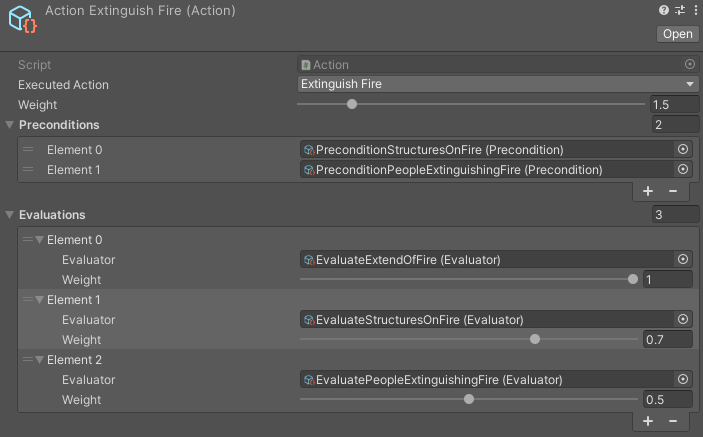
\includegraphics[scale=0.5]{images/utility_ai_scriptableobject_action.png}
	\caption{ScriptableObject for the extinguish fire action}
	\label{fig:utility_ai_scriptableobject_action}
\end{figure}

This is a ScriptableObject of the Action class, representing the extinguish fire action. At the top, the action to be performed and its weigh can be selected. Directly below this are the preconditions, in this example, the action to extinguish fire will only be considered if at least one structure is on fire and no one else is already doing this action. Finally, all the evaluations are listed, with each element consisting of an evaluator and its corresponding weight.

Using ScriptableObjects for actions has the advantage of allowing new preconditions and evaluators to be easily added within the Unity editor without the need for any additional coding. It's also clear which action has which components. The ScriptableObjects for the other utility AI elements look similar, but with different fields.

\newpage

\section{Examples}
\label{sec:utilityai_examples}
\subsection{Daily Routine}
\label{subsec:utilityai_realization_dailyroutine}

The first and simpler example shows an agent trying to live a normal daily routine. This routine consists of only three activities: working, eating and sleeping.

\begin{figure}[H]
	\centering
		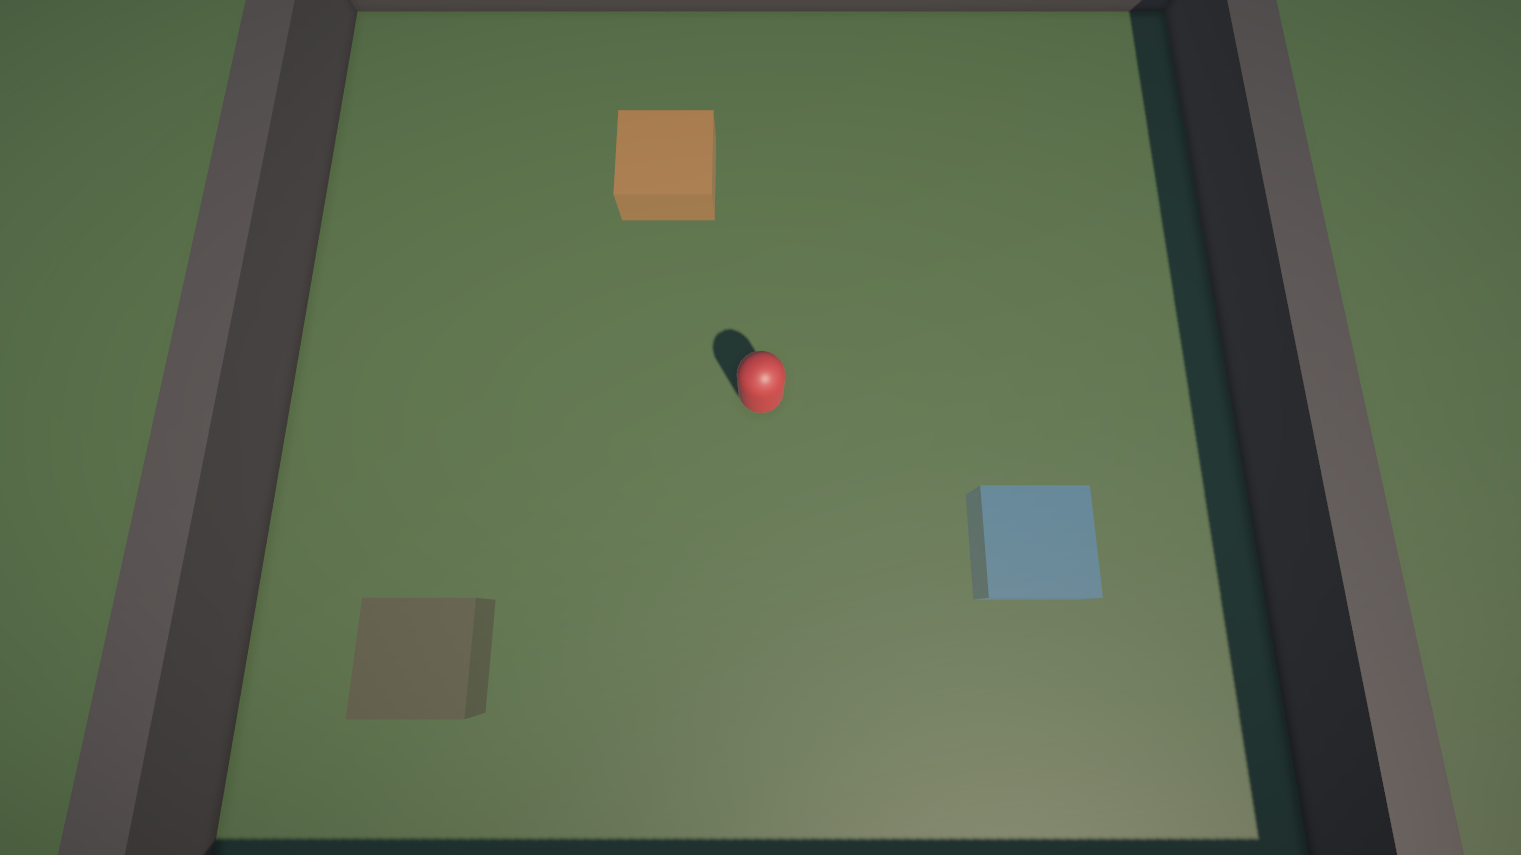
\includegraphics[scale=0.3]{images/utility_ai_scene_daily_routine.png}
	\caption{Scene in Unity for the agent's daily routine}
	\label{fig:utility_ai_scene_daily_routine}
\end{figure}

Each of these cubes represents a building in which the agent can perform a specific action: brown for working, orange for eating and blue for sleeping. Obviously, it can only do one action at a time, and it has to decide which one it wants to do by using the utility AI. The agent gradually loses saturation and energy over time, which can be regained by eating or sleeping. To eat, the agent must spend money on food, which it can earn by working. Sleeping and working both take time, while eating is instantaneous.

\begin{figure}[H]
	\centering
		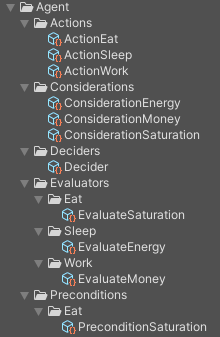
\includegraphics[scale=0.6]{images/utility_ai_daily_routine.png}
	\caption{Structure of the utility AI for the agent}
	\label{fig:utility_ai_daily_routine}
\end{figure}

The agent has three actions, each of which depends on only one evaluator. The action eat also has a precondition, which forbids the agent to eat if its saturation is above 90. With this structure, the agent is always able to choose the best action in this very simple world.

\newpage

\subsection{Spaceship}
\label{subsec:utilityai_realization_spaceship}

In this example, two spaceships with different elements on them are trying to attack each other. The following elements on the spaceships can be controlled by the two agents operating them:

\begin{tabular}{lp{12cm}}
Quarters: & The place where the agents sleep. \cr
Factories: & The place to produce materials that can be used as ammunition or to repair the ship. \cr
Storage: & The place where materials can be stored in larger quantities. \cr
Cannon: & The location from which the enemy spaceship can be fired at, using ammunition \cr
Fire Extinguisher: & The place where the fire extinguisher can be picked up to put out fires caused by enemy attacks.
\end{tabular}

There are also two other structures that are not intended to be operated by an agent:

\begin{tabular}{lp{12cm}}
Shields: & These elements are more resistant to enemy attack than any other structure. \cr
Paths: & The way for agents to walk from point A to point B.
\end{tabular}

\begin{figure}[H]
	\centering
		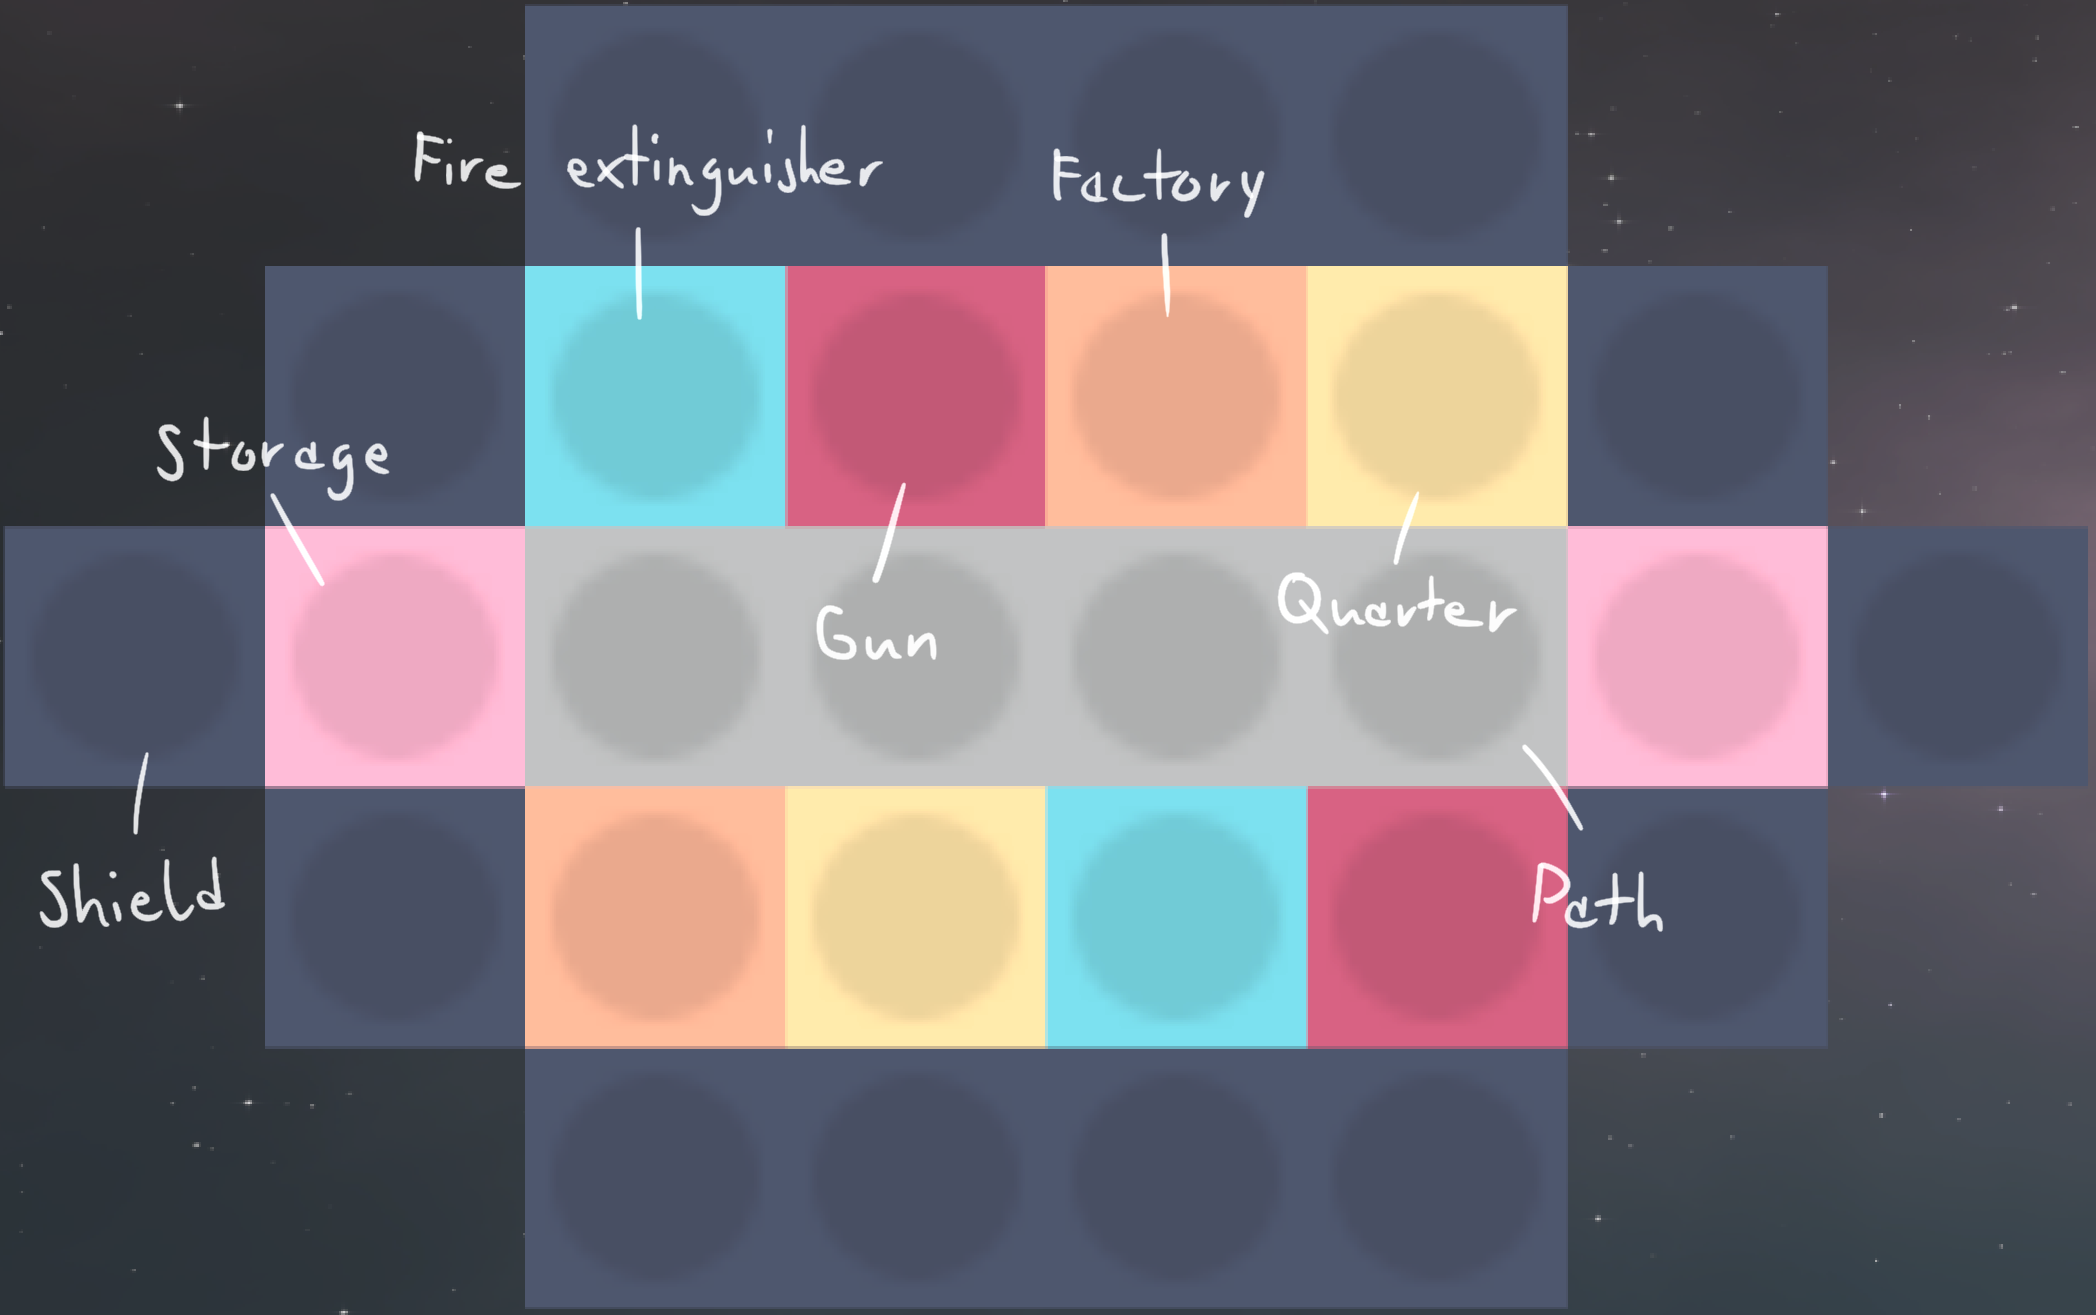
\includegraphics[scale=0.21]{images/utility_ai_scene_single_spaceship.png}
	\caption{Close up view of a single spaceship in Unity}
	\label{fig:utility_ai_scene_single_spaceship}
\end{figure}

In order for an agent to perform a certain action, it must first go to the specific structure. Once there, it can start performing the desired action. The agent can only use path elements to reach a new location, and navigation is done using Unity's NavMesh. Performing an action takes a fixed amount of time, which differs for each action.

A structure loses health points (HP) over time, depending on the extent of fire on that structure. Attacking the enemy spaceship means increasing the extent of fire on an enemy structure. Each shot increases the intensity by a certain amount. When a structure reaches 0 HP, it is marked as destroyed. Destroyed structures cannot be used to perform actions, but they can be repaired by taking some materials from the storage and using them to repair the structure.

\newpage

The actions available to the agent are shown in the following figure:

\begin{figure}[H]
	\centering
		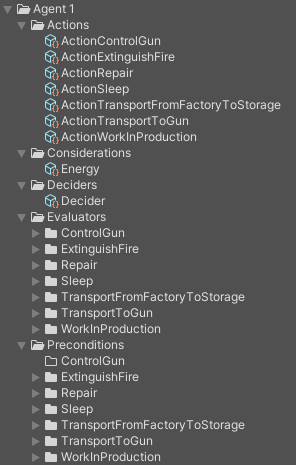
\includegraphics[scale=0.6]{images/utility_ai_spaceship.png}
	\caption{Structure of the utility AI for one agent}
	\label{fig:utility_ai_spaceship}
\end{figure}

To make it easier to understand, here is an example scenario: the agent starts by going to the factory to produce some materials. Once it's got some materials, it will choose to move those items to the warehouse, so that there's enough space in the factory to produce new items. After it has some items, it will move some of them to the cannon and start shooting at the enemy ship with the ammunition. At this point, it is likely that the enemy ship will start firing back as well, which will put the attacked structures on fire. The agent will then grab the fire extinguisher to defend his ship. If there are already destroyed structures, the agent might consider repairing them instead of doing other actions. It is also important to remember to sleep from time to time, otherwise its movement speed will be significantly reduced when it s too tired.

The spaceship will always have two copies of the same structure on board, as it is forbidden for more than one agent to perform the same action in the same place.

\begin{figure}[H]
	\centering
		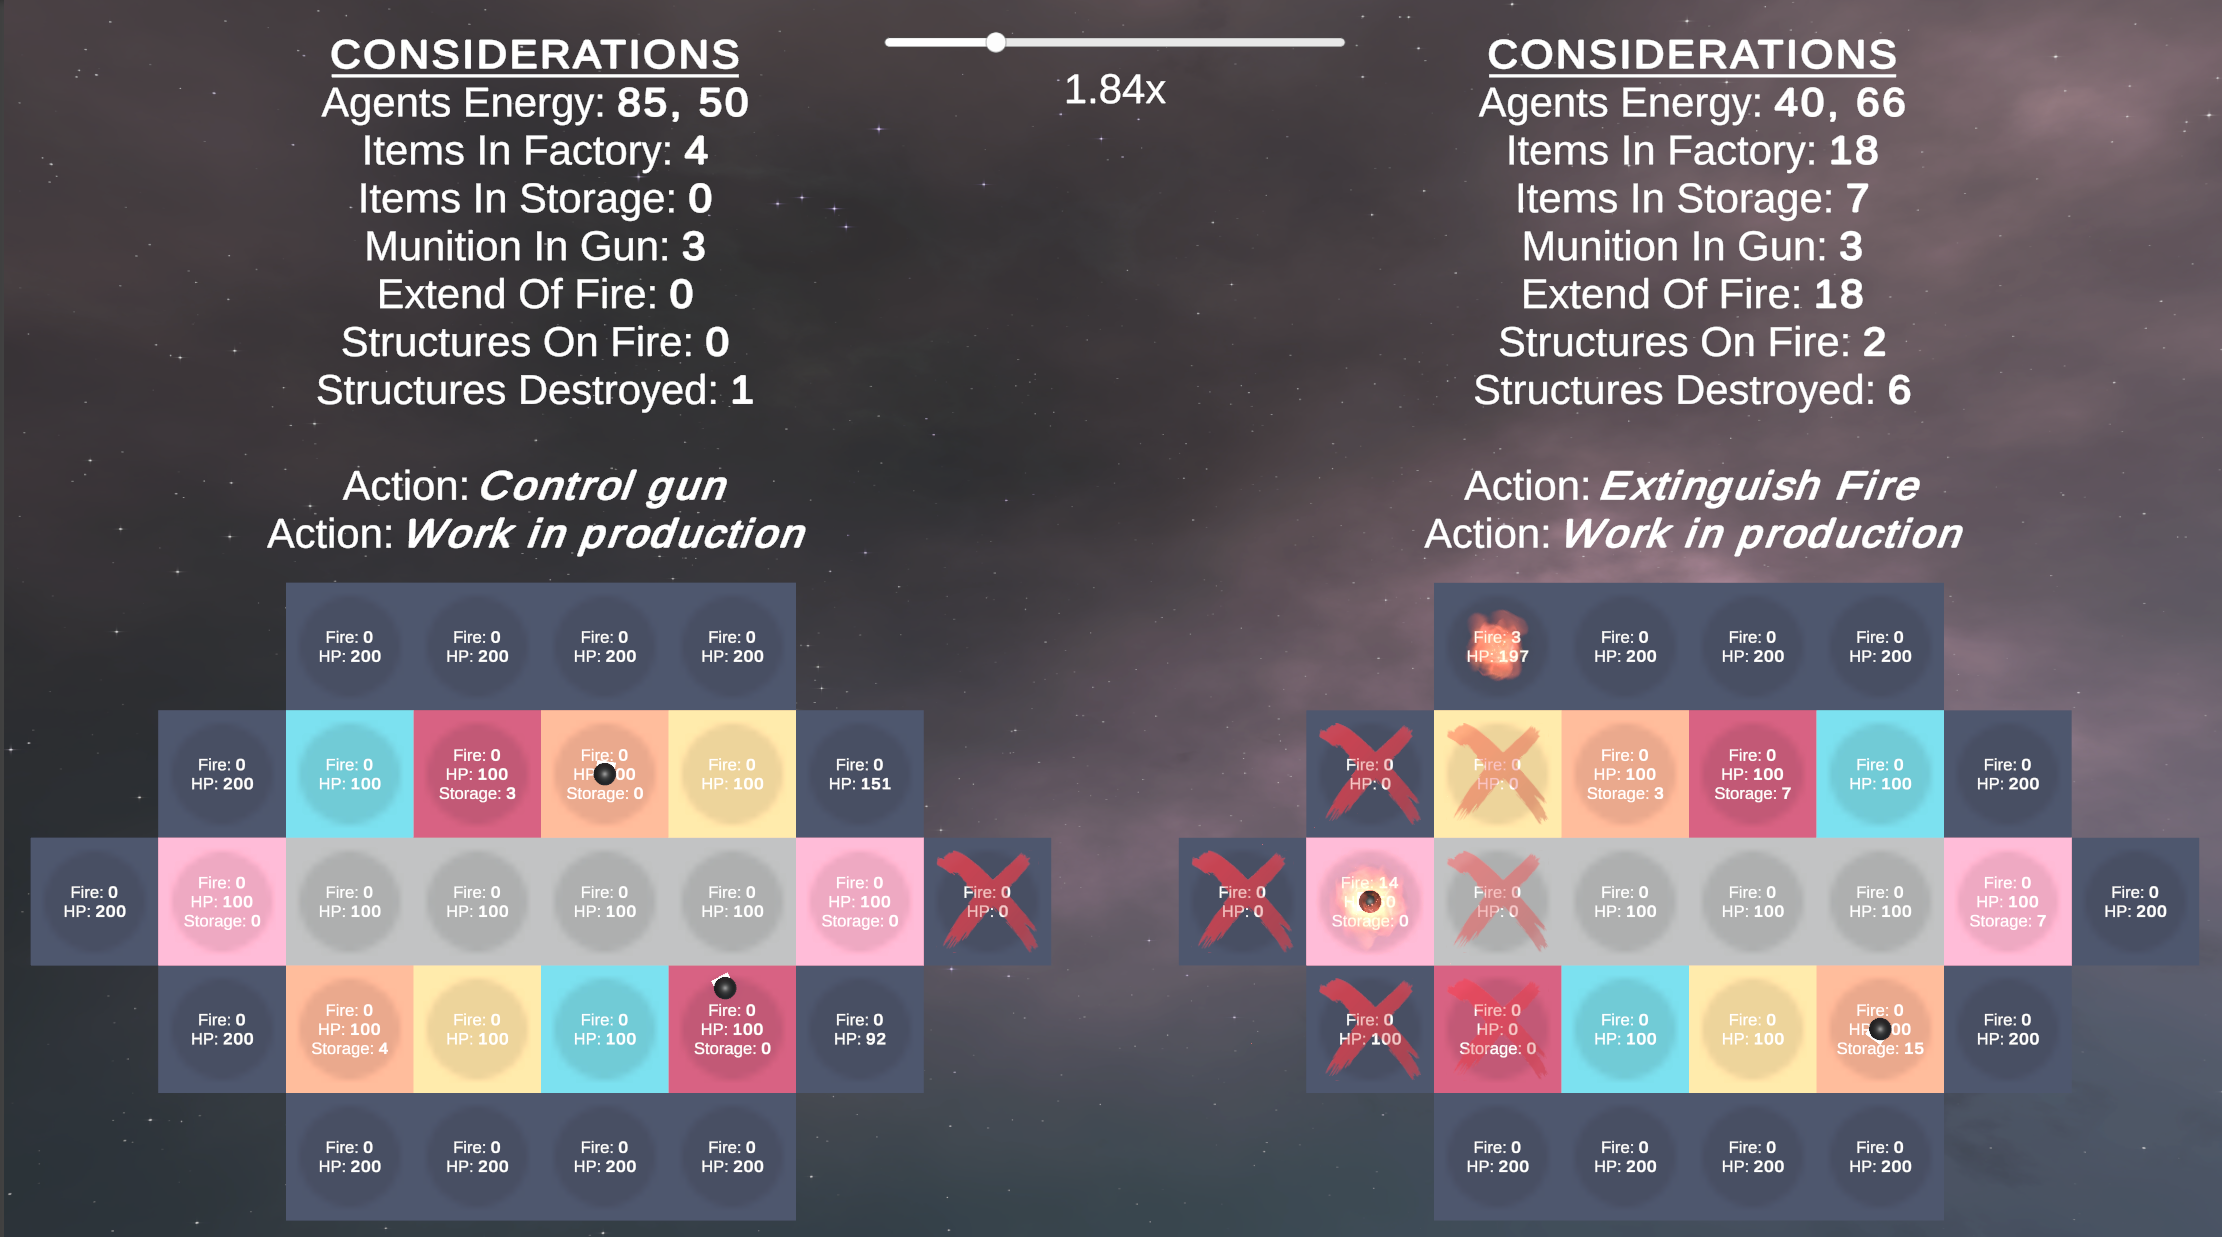
\includegraphics[scale=0.265]{images/utility_ai_scene_both_spaceship.png}
	\caption{Scene in Unity showing an ongoing battle}
	\label{fig:utility_ai_scene_both_spaceship}
\end{figure}

Figure \ref{fig:utility_ai_scene_both_spaceship} shows a screenshot of an ongoing battle between the two ships. At the top you can see the considerations of each spaceship, and just below them the current actions of the two agents. The crossed objects symbolise that they have been destroyed, and the burning ones are on fire. The extent of fire and its HP can be read in the overlay. It looks like the left spaceship is attacking, while the other is trying to defend itself by extinguishing fires and preparing materials for repair or counter-attack.

\newpage

\section{Strengths}
\label{sec:utilityai_strengths}

Utility AI is very good at making intelligent and realistic decisions based on the current state of the environment. It only lives in the present and doesn't care about what might happen afterwards. So utility AI becomes a very powerful tool when the agent has a lot of decisions to make and considerations to take into account, but doesn't have to worry about later decisions.

This tool also excels in its modularity. New actions can be added at any time during development without disturbing the others, and without having to change any of them to make them fit. The same goes for the evaluators. Because of the way the scores of the evaluators are calculated, new evaluators can be freely added to make the agent consider a new aspect of the game. This can be useful if, for example, a new feature has been added to the game during development, and the agent needs to take this into account when making a decision. It can also be very helpful when trying to find the most appropriate behaviour for an agent to be able to freely remove or add existing evaluators.

Thirdly, the weights of the actions combined with the weights of the evaluators can lead to very simple and fast changes in the behaviour of each agent. In the example of the defending agent from figure \ref{fig:utility_ai_sketch_defending_ai_with_values}, if the weights for the actions "heal" and "reload" are changed to 2 and "attack" to 3, the agent will play much more aggressively and will most likely change the order of the actions to "cover", "reload" and finally "attack". On the other hand, if the weight for the "attack" action is changed to 3 and its EH (enemy health) evaluator to 50\% weight, the AI will prioritise attacking enemy units with low health. Because it's so easy to change weights or even curves with just a few clicks, many different characters can be created from the same basic structure in no time, resulting in much more realistic and interesting NPCs.

\section{Weaknesses}
\label{sec:utilityai_weaknesses}

As mentioned previously, utility AI only considers its current environment and doesn't know what future actions might be. This makes it poor at planning ahead. This could be compensated by giving the NPC considerations that try to represent the future. However, since this consideration also depends on the action the NPC will choose, it will be very difficult to implement, and therefore isn't well supported by the framework.

It also struggles with sequential behaviour, like that of a tour guide. Since there are no states to switch to, all states would have to be represented by actions and considerations that change their value based on the current state. This would make the whole architecture more complex than it needs to be, whereas a simple FSM or behaviour tree would probably do the job.
\chapter{Comparison To Other Solutions}
\label{chap:comparisontoothersolutions}

\section{Goal Oriented Action Planning}
\label{sec:comparisontoothersolutions_goalorientedactionplanning}

With Goal Oriented Action Planning (GOAP), the agent is able to plan the best sequence of actions, depending on the current state of the environment, to achieve a given goal as efficiently as possible. It can generate different action plans, evaluate their costs, and then choose the one that best fits the current circumstances. Every plan can consist of several actions, each associated with a weight to help the agent decide on the best sequence. \cite{GOAP}

A good example is the goal for an agent to get apples. Suppose there are three actions the agent could perform: pick the apple, grab ladder and buy apples. To perform the action of picking an apple, the agent first needs a ladder, otherwise the apple is out of reach. The actions can be given an individual cost:

\begin{tabular}{lp{12cm}}
pick apples: & 3 cost \cr
grab ladder: & 4 cost \cr
buy apples: & 8 cost
\end{tabular}

Now there are two different sequences of actions that the agent can choose from to achieve his goal of getting apples:

\begin{tabular}{lp{12cm}}
grab ladder -> pick apples: & total cost: 7 \cr
buy apples: & total cost: 8
\end{tabular}

Because the sequence of actions of grabbing his ladder and then picking apples has a lower cost than buying apples, it would choose that sequence. However, if the cost of the ladder increases because the ladder is broken and the agent would have to fix it first, then it might decide to just go and buy some apples because the cost of doing so is lower.

Also, the agent could learn a new skill that allows him to climb trees at a cost of only 2. With GOAP, this new action could then simply be added to the other actions, and the framework would take it into account when making decisions. As a result, the agent would never need to use the ladder again.
In order for the framework to plan its actions, each action must have preconditions and effects. Similar to utility AI, preconditions must be met for an action to be executed. Effects, on the other hand, are NOT the executed behaviour, they only represent the state that would be achieved if this action were executed. Effects are only used by the GOAP planner to plan ahead. As an example, the actions could have the following preconditions and effects, where "has apples" is the goal:

\begin{tabular}{lp{12cm}}
pick apples: & Preconditions: "in range to pick" | Effect: "has apples" \cr
grab ladder: & Preconditions: "ladder available", "doesn't have ladder" | Effect: "in range to pick" \cr
buy apples: & Preconditions: "shop is open" | Effect: "has apples"
\end{tabular}

\newpage

With this information, the GOAP planner can now iterate through all possible sequences of actions to find the path with the lowest cost. It will also look at sequences that don't make much sense, like "grab ladder" -> "buy apples". But since the cost is too high with (4 + 8) = 12, it will not be chosen. Buying apples directly is always cheaper. \cite{GOAP}

This solution is closest to utility AI because it's also able to react intelligently without having to script every possible situation, resulting in more dynamic behaviour. The GOAP cost system is analogous to the utility AI score system. The main difference is that GOAP is goal based and creates an optimal sequence of actions and then executes them one by one. Utility AI, on the other hand, will always choose the action that best suits the current situation, without making a plan for the next actions. Depending on the implementation, there may be other differences, such as how costs and points are calculated. Also, the way information from the world is evaluated with curves in utility AI may be different when using GOAP.

\section{Reinforcement Learning}
\label{sec:comparisontoothersolutions_reinforcementlearning}

Reinforcement learning (RL) is a machine learning model where the agent can learn from an interactive world by trying and learning from the outcome. With RL, the programmer no longer needs to specify the weights for how important which action is. Instead the agent will figure it out by trying different approaches and then getting rewarded or punished for the outcome. \cite{RL}

Reinforcement Learning is a machine learning model where the agent can learn from an interactive world by trying and learning from the result. With RL, the programmer no longer needs to specify weights for how important an action is. Instead, the agent figures it out by trying different approaches and then being rewarded or punished for the outcome.

\newpage

\section{Overview Of All Solutions}
\label{sec:comparisontoothersolutions_overviewofallsolutions}

\begin{figure}[H]
	\centering
		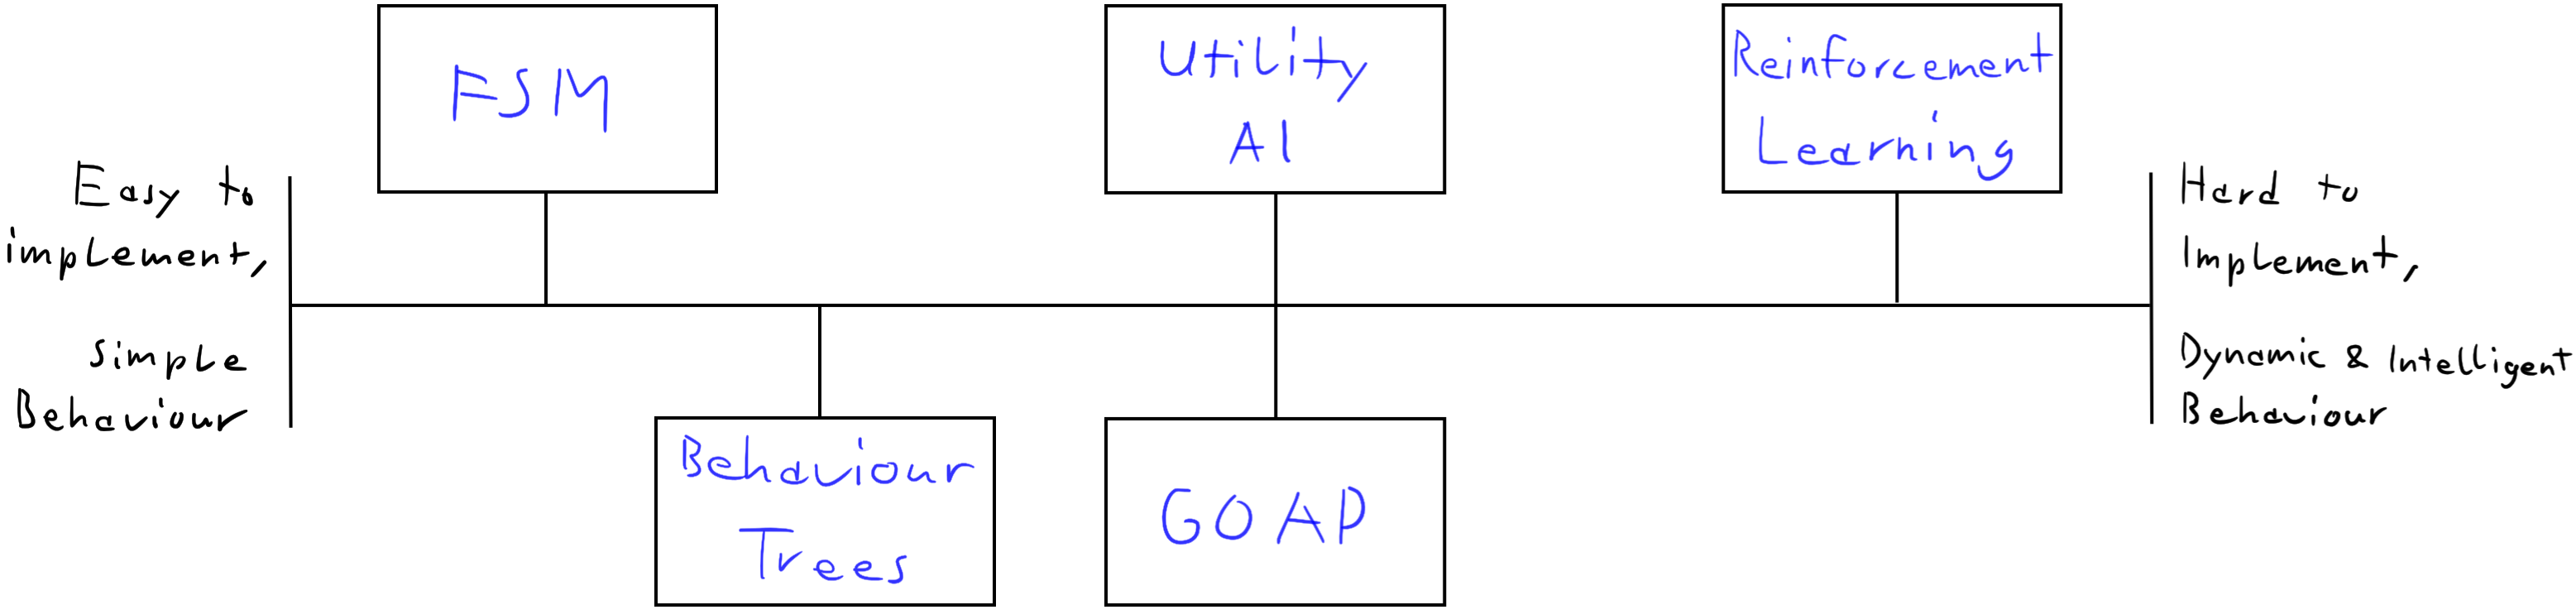
\includegraphics[scale=0.19]{images/comparison_of_ai_solutions.png}
	\caption{Comparison of solutions used for NPCs \cite{Comparison}}
	\label{fig:comparison_of_ai_solutions}
\end{figure}

This sketch shows all the solutions presented in this paper, from those that are easy to implement and understand, to those that are more complex but will result in more intelligent behaviour. There is no "best solution" for every situation. Depending on the problem, the right solution needs to be chosen, and utility AI is just one of them.

The requirements for an NPC depend very much on how complex it needs to be, and what kind of behaviour is required. For a very simple scenario, an FSM might be just fine, and it's also very easy to implement. But for more complex behaviours, it's often worth the time to learn or even implement a more complex solution.

A developer must also consider the performance of the application. If you have a game with hundreds of zombies running towards the player, it might be too expensive to give each one the ability to decide the best sequence of actions using, for example, GOAP. It would also take more time to implement, and on top of all, the player might not even notice the intelligence of the enemies because they are too many and die with a few shots anyway.
\chapter{Utility Designer}
\label{chap:utilitydesigner}
\section{Introduction}
\label{sec:utilitydesigner_introduction}

There are many solutions available for creating AIs, and it is important for developers to have a good set of tools. At the moment there are some really good assets in the Unity Asset Store for FSMs and behaviour trees, as the concept has been around for a long time. However, for implementations of more dynamic behaviours, such as utility AI, there is not as much to be found.

The tool developed in this thesis, called Utility Designer, aims to fill this gap by providing a generic and intuitive tool that uses a combination of utility AI and behaviour trees. Utility AI is used to decide the best state, where each state has a behaviour tree that defines the specific actions and behaviours of that state. This combination allows the NPC to make decisions on their own, while still being able to define the execution of states with familiar behaviour trees.

A crucial aspect of designing a tool for others is to effectively communicate how it works, as users may have no prior knowledge of it. Not only is it important to keep the tool simple by hiding complex structures behind an intuitive and pleasing interface, but it must also provide a quick way for a new user to learn how it works. This is a key component of any tool, as its purpose is to save programmers time by doing some of the work for them. It is therefore essential to provide a manual, sample scenes, a tutorial video, etc.

A manual explaining everything about Utility Designer can be found in the appendix to learn more about how the tool works.

\section{Use Cases}
\label{sec:utilitydesigner_usecases}

The ideal use case is where NPCs need to make dynamic decisions based on the current situation, where they cannot simply follow fixed rules. It thrives when multiple factors influence an NPC's behaviour and decision-making process. Here are some different use cases for Utility Designer:

\paragraph{Expandability:}
When making a game or simulation, sometimes new features are added that give NPCs a new state to choose from, such as the option to go swimming. In Utility Designer, adding a new state is enough for the NPC to include it in their decision making. There is no dependency on the complexity of the structure and the amount of choices the NPC has, because all the other states do not need to be touched when you add a new one. Doing something like this in a state machine or behaviour tree might not be so straightforward.

\paragraph{Built-in Behaviour Tree:}
In a situation where utility AI is not required, for example when creating sequential behaviour for a tour guide, Utility Designer offers the option of using the tool as a normal behaviour tree. This can be achieved by simply using one state without any preconditions and then using its behaviour tree to create the desired behaviour. This behaviour tree will then always be executed as it is the only state that can be selected.

\paragraph{Multiple NPCs:}
If there is a need to create multiple instances of the same character, NPCs with a Utility Designer component on them can simply be copied and pasted, or instantiated from a prefab. They will then share the same behaviour rules, which can be useful for something like a group of monsters.

\paragraph{Dynamic Environments:}
In video games or simulations where things change a lot, utility AI helps NPCs make good decisions. They check things like how close enemies are, if there are resources nearby, or what's happening at important locations. The decisions are then made by the NPCs themselves, which makes them feel more real.

\paragraph{Easy To Adjust:}
Imagine a scenario where a small village should be populated with different kinds of NPCs to make the village feel alive to the player. Most states are shared by all the NPCs, such as "Sleep", "Eat", "Read newspaper" "Walk around", "Talk" and so on. These states only need to be created once and can then be used by any NPC. The behaviour can then be copied, and a few weights or states can be changed, making it incredibly easy to create unique personalities for different characters. One of them might for example be an introvert, and have their weights for "Walk around" and "Talk" a bit lower, while the state "Read newspaper" is weighted more.

\section{Implementation}
\label{sec:utilitydesigner_implementation}

\subsection{Technology Stack}
\label{sec:utilitydesigner_implementation_technologystack}

\subsubsection{Overview}
\label{sec:utilitydesigner_implementation_technologystack_overview}

The Utility Designer uses different technologies to facilitate a synergistic relationship between utility AI and behaviour trees, simplifying the process of generating advanced and dynamic behaviours. Unity and C\# have both been around for some time, making them mature and well-established technologies. Despite their longevity, they are still actively maintained and updated to reflect new advances in software development. Unity's UI toolkit, on the other hand, is relatively new and continues to be actively developed.

\subsubsection{Unity}
\label{sec:utilitydesigner_implementation_technologystack_unity}

Unity is the base layer of the tool. Utility Designer is built in Unity because Unity's Asset Store is a good way to share tools and assets with other developers. The latest version of Unity used is 2022, as each version adds more features to the UI toolkit, and it's the latest stable release to date. This cross-platform game engine is used as the basis for all development activities. Robust, feature-rich and versatile, Unity serves as the cornerstone in the creation and operation of the Utility Designer, handling everything from 3D environment rendering and user input management to game physics.

\subsubsection{C\#}
\label{sec:utilitydesigner_implementation_technologystack_csharp}

The core logic of Utility Designer is written in C\#, a powerful object-oriented programming language. C\# is used to implement the utility's AI and behaviour tree logic, and to manage interactions with the user interface. This programming language provides access to a wide range of libraries and features, allowing a high degree of customisation and control over the project structure.

\subsubsection{Unity's UI Toolkit}
\label{sec:utilitydesigner_implementation_technologystack_unitysuitoolkit}

Unity provides a system for creating editor windows called UI Toolkit. It is used to create a visually appealing and interactive user interface. The UI Toolkit is a flexible and efficient system for building UI in Unity and is used to create a rich, yet simple and user-friendly graphical interface for the Utility Designer. The toolkit allows the UI to be designed using UXML and USS, languages similar to HTML and CSS respectively, allowing for highly flexible and scalable UI design.

\subsection{Software Architecture}
\label{sec:utilitydesigner_implementation_softwarearchitecture}

The architecture of Utility Designer has been designed so that it has no dependencies outside of its own folder, allowing the folder to be freely moved around without any problems. In addition, users do not need to interact with or write scripts within this folder, and its own assembly definition ensures that the tool remains self-contained.

Splitting the code into different namespaces significantly reduces dependencies throughout the project, making it easier to maintain. Three particular namespaces stand out as the most important.

\begin{tabular}{lp{12cm}}
Evaluation: & This namespace contains the functionality for the evaluation tab and implements the logic and calculations of utility AI, as well as the considerations. \cr
Execution: & Used for the implementation of the behaviour tree found in the execution tab. It also contains all the various predefined nodes and the SceneReferences script. \cr
Editor: & Here are all the UXML and USS documents needed to visualise the different editor windows, as well as some C\# scripts to add logic such as user interaction and runtime debugging. This folder is ignored by Unity during runtime builds to save resources.
\end{tabular}

Outside of these namespaces is the UtilityDesigner script which holds the logic to initialise and update the evaluation and execution tab according to the specified tick rate. It is also responsible for the safe, load and log functions.

The design of the tool is not focused on optimising the example scenes. Furthermore, these scenes are not housed within the UtilityDesigner assembly, but are external to it, as they are not directly related to the core functionality of the tool. They simply use Utility Designer from an external position, reflecting the scenario of a developer who has included Utility Designer in their project as a standalone tool to increase production speed.

\subsection{Discarded Concepts}
\label{sec:utilitydesigner_implementation_discardedconcepts}

Developing tools can sometimes be tricky, especially when doing it for the first time, because a tool like Utility Designer has to provide different aspects for the developer to speed up their production, while still remaining generic, intuitive and maintainable. Therefore, some concepts were not completely clear from the start. Different approaches were tested to find the best one.

\paragraph{Scene References:}
One of the key decisions was to store the behaviour as a ScriptableObject, making it easy to maintain as it can be duplicated and freely attached and removed from the UtilityDesigner script. One of the characteristics of ScriptableObjects is that no references from the scene can be stored in them. However, it is important for the action nodes to have access to references from the scene, such as the location of the NPC's house or the enemy. Hence the concept of the SceneReferences script. But before that, there were other ideas to solve this problem:

\begin{tabular}{lp{12cm}}
Inspector: & The most intuitive way would be to drag and drop the references to the node inspector. As these references cannot be saved in the ScriptableObject, the name of the GameObject could be stored instead as a workaround. However, this creates a problem if two or more of these references have the same name, as they can no longer be clearly distinguished by name alone. And trusting the user not to give the same name to two GameObjects in their scene that are used in a behaviour tree is too risky. \cr
Event manager: & Instead of making action nodes based on separate scripts, another approach could be to have a static event manager. The user could then subscribe to events from the manager, and these events would be fired each time the action node is invoked. The problem with this approach is that the main advantage of action scripts is lost: the ability to re-use the same code for different behaviours with the click of a button. It also makes it difficult to encapsulate parts of the code with a single giant event manager, which could make the code organisation of a large project worse.
\end{tabular}

Considering these ideas, the best approach was to create a script called SceneReferences, which contains all the references needed for a UtilityDesigner. This script can then be attached to a GameObject in the scene and the name of the GameObject is stored in the ScriptableObject. References from SceneReferences can then be easily accessed in the action nodes in the node inspector or through a provided API. This makes it possible to have separate scripts for the action nodes without having to trust the end user. SceneReferences are not restricted to the behaviour tree and can be used elsewhere in the project.

\newpage

\paragraph{Execution Tab:}
It was not clear from the start what the execution tab would look like, and different ideas were considered depending on the time available for implementation:

\begin{tabular}{lp{10cm}}
Link other implementations: & If there was no time for the execution tab, there should at least have been a way to link to other assets, such as a behaviour tree asset. Fortunately, there was enough time to implement a useful framework. \cr
State Machine: & The first idea used was an implementation of a state machine, because it is quite easy to implement. But the more the tool was tested, the more it became clear that loops are used very often in the execution tab, and state machines are not the best thing for that, as shown in the section \ref{sec:projectevolution_whyitfails}. \cr
Behaviour Tree: & Since there was still time for a more complex framework, and the scene reference problem wasn't solved yet, it seemed like a good opportunity to start implementing a behaviour tree. They are very flexible and well known among AI developers, which makes it easier for them to get started with Utility Designer. \cr
GOAP: & Goal Oriented Action Planning could also be a possible approach for executing states, as the evaluation tab could decide the goal, and GOAP would plan how to execute it. The problem is that GOAP is harder to get started with than BTs, and in many cases a simple sequence of actions is sufficient for a state, making the added complexity of GOAP unnecessary.
\end{tabular}

\begin{figure}[H]
	\centering
		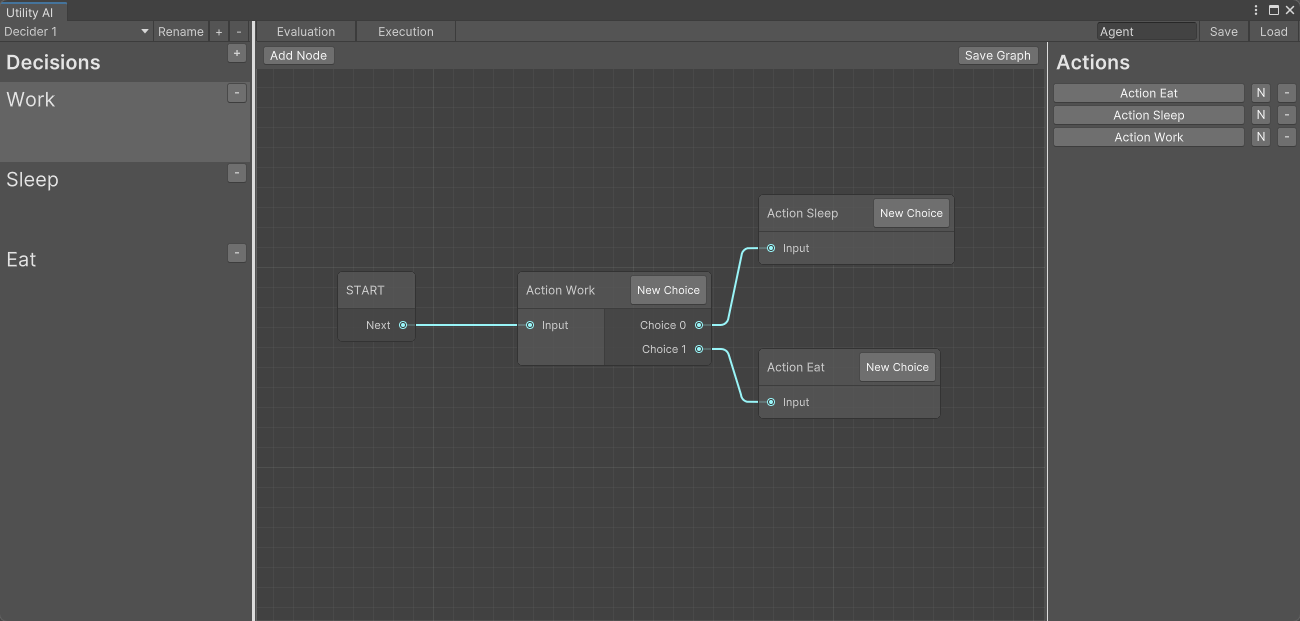
\includegraphics[scale=0.38]{images/utility_designer_state_machine.png}
	\caption{Discarded implementation of a state machine}
	\label{fig:utility_designer_state_machine}
\end{figure}

However, there is always the option to use a custom framework to execute nodes, simply by using an action node in the execution tab, which then calls the external framework to execute the state.

\newpage

\subsection{Third Party Code}
\label{sec:utilitydesigner_implementation_thirdpartycode}

In order to speed up the development process and achieve more goals, the help of some external tools and websites have been included. Extensive research was conducted across multiple websites such as Unity's documentation (Unity Docs)\footnote{\url{https://docs.unity.com}}, YouTube tutorials, especially this one for the behaviour tree (YouTube)\footnote{\url{https://youtu.be/nKpM98I7PeM}} and (Stack Overflow)\footnote{\url{https://stackoverflow.com}}, among others.

In addition, the AI-powered tool, ChatGPT (ChatGPT)\footnote{\url{https://chat.openai.com}}, and the autocorrect functionality provided by JetBrains' IDE for C\#, known as Rider (JetBrains Rider)\footnote{\url{https://www.jetbrains.com/rider/}}, were instrumental in improving efficiency and code quality.

Apart from the author and supervisor of this thesis, no one else contributed to the code. However, it is worth noting that the basic idea of how utility AI is implemented comes from Project 2, the previous project before the thesis.

\section{Example Scenes}
\label{sec:utilitydesigner_implementation_examplescenes}
\subsection{Daily Routine}
\label{sec:utilitydesigner_implementation_examplescenes_dailyroutine}

The first and simpler example again shows an agent trying to live a normal daily routine. Everything is the same as in section \ref{subsec:utilityai_realization_dailyroutine}, except that the house is white instead of blue, and the consideration saturation has been renamed to hunger to keep consistency with the second example scene.

\begin{figure}[H]
	\centering
		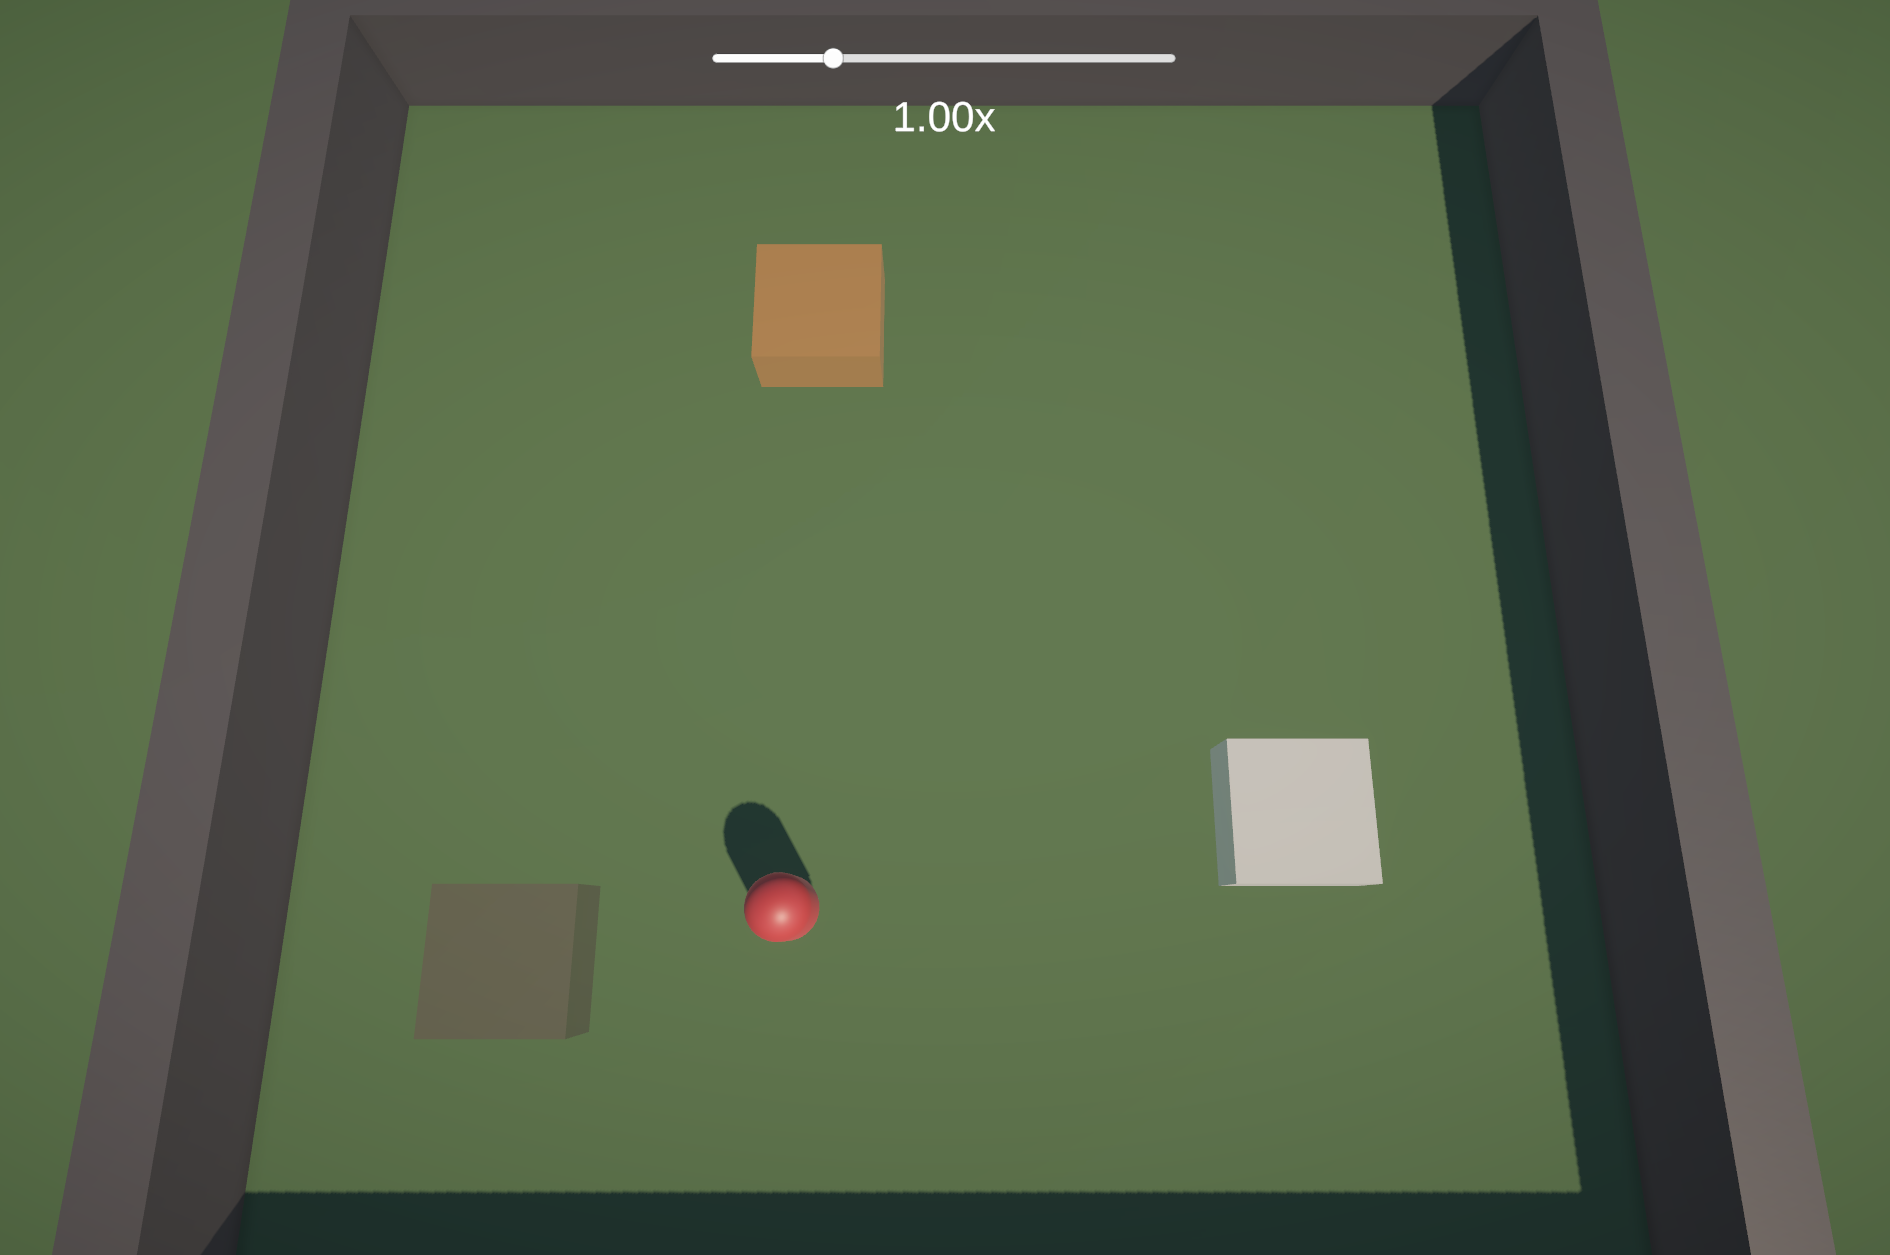
\includegraphics[scale=0.2]{images/utility_designer_daily_routine.png}
	\caption{Scene in Unity for the agent's daily routine}
	\label{fig:utility_designer_daily_routine}
\end{figure}

\newpage

The behaviour for this scene using Utility Designer is as follows:

\begin{figure}[H]
	\centering
		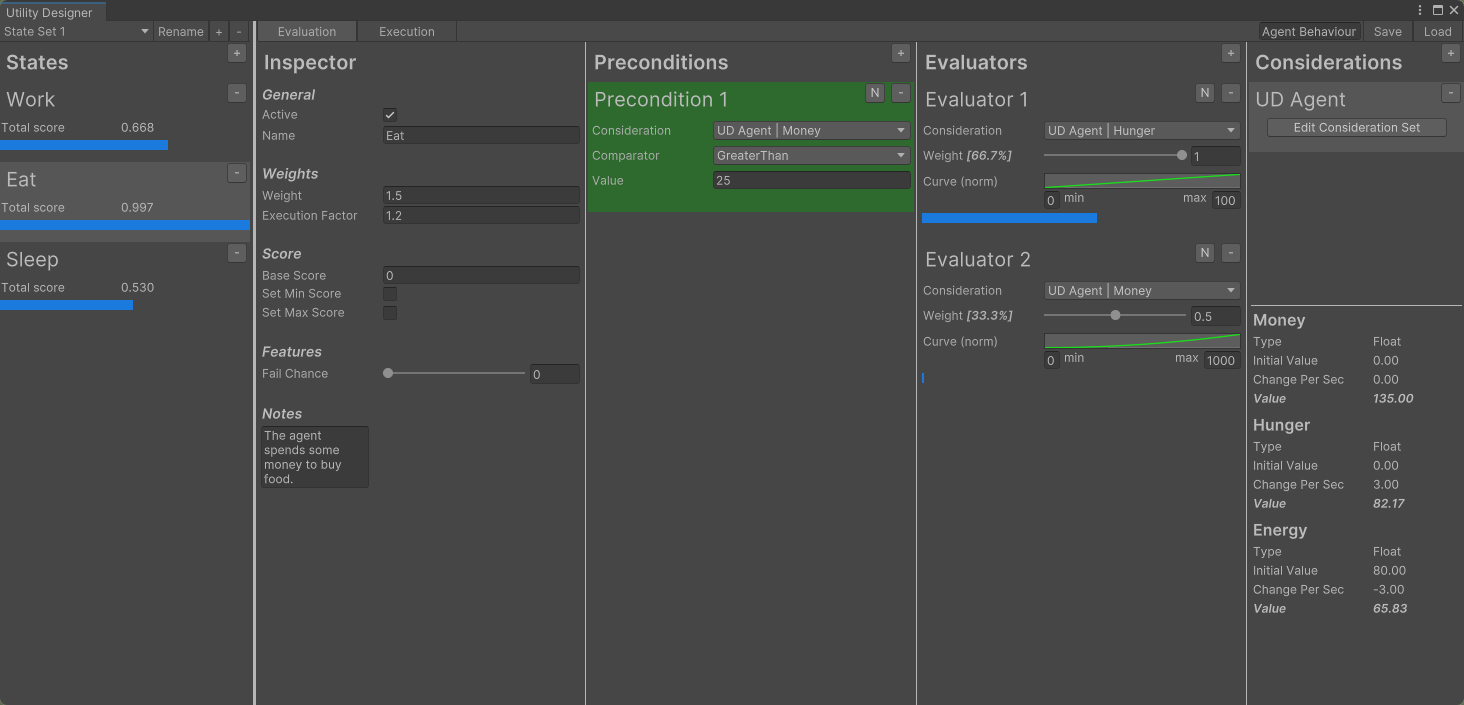
\includegraphics[scale=0.38]{images/utility_designer_daily_routine_evaluation.png}
	\caption{Evaluation tab for the agent in Utility Designer}
	\label{fig:utility_designer_daily_routine_evaluation}
\end{figure}

The figure \ref{fig:utility_designer_daily_routine_evaluation} shows the evaluation tab with the "Eat" state selected. This state is evaluated using hunger and money, with hunger having twice the weight of money. To eat, the agent must have at least enough money to buy one meal.

\begin{figure}[H]
	\centering
		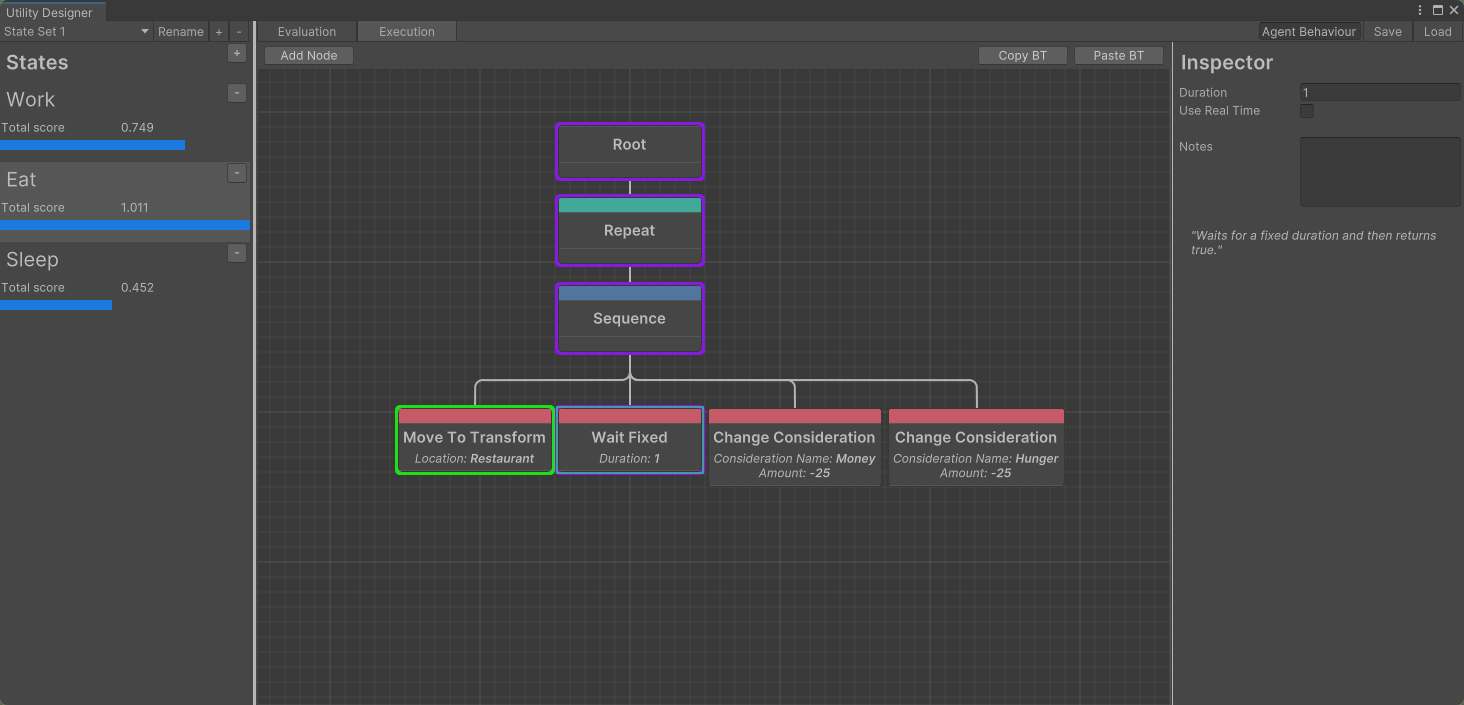
\includegraphics[scale=0.38]{images/utility_designer_daily_routine_execution.png}
	\caption{Execution tab for the agent in Utility Designer}
	\label{fig:utility_designer_daily_routine_execution}
\end{figure}

The Execution tab looks fairly straightforward. There is only one repeating sequence, which makes the agent go to the restaurant if he has not already done so, and pay 25 money to lose 25 hunger, repeated every second. The other states look pretty similar, just changed to suit the state.

\newpage

\subsection{Survival}
\label{sec:utilitydesigner_implementation_examplescenes_survival}

In the survival scene, the NPC called James has to survive as long as possible by efficiently choosing which task is best given the current circumstances. James will die either by being eaten by a bear or by starvation. James has the following states:

\begin{tabular}{lp{12cm}}
Fish: & Gets food slowly at a random rate and is always successful. \cr
Hunt: & Attempts to kill a deer to get a lot of food quickly, but the chance of success decreases the less energy and strength he has. Needs a deer nearby. \cr
Sleep: & Takes a nap to restore energy over time. \cr
Eat: & Roasts and eats meat from fishing and hunting to reduce hunger. \cr
Work out: & Builds up strength over time. Cannot be done if motivation is too low. Reduces motivation and energy. \cr
Fight: & Sometimes a bear will attack him. Will die if he does not have enough strength. \cr
Play: & Increases motivation over time. Cannot play if too hungry. \cr
\end{tabular}

Two different consideration sets were used to evaluate the states. One is specific to the needs and desires of James, and a global one is used to represent the environment. The consideration set for James is local, because it is specific to each instance of James, if there were more than one. It contains the considerations "Hunger", "Energy", "Food", "Motivation" and "Strength". The consideration set about the environment only has two considerations: "Deer nearby" and "Bears nearby".

The scene was created using the Low Poly Ultimate Pack Asset, which contains many low-poly pre-built assets to help create decent-looking scenes quickly.

\begin{figure}[H]
	\centering
		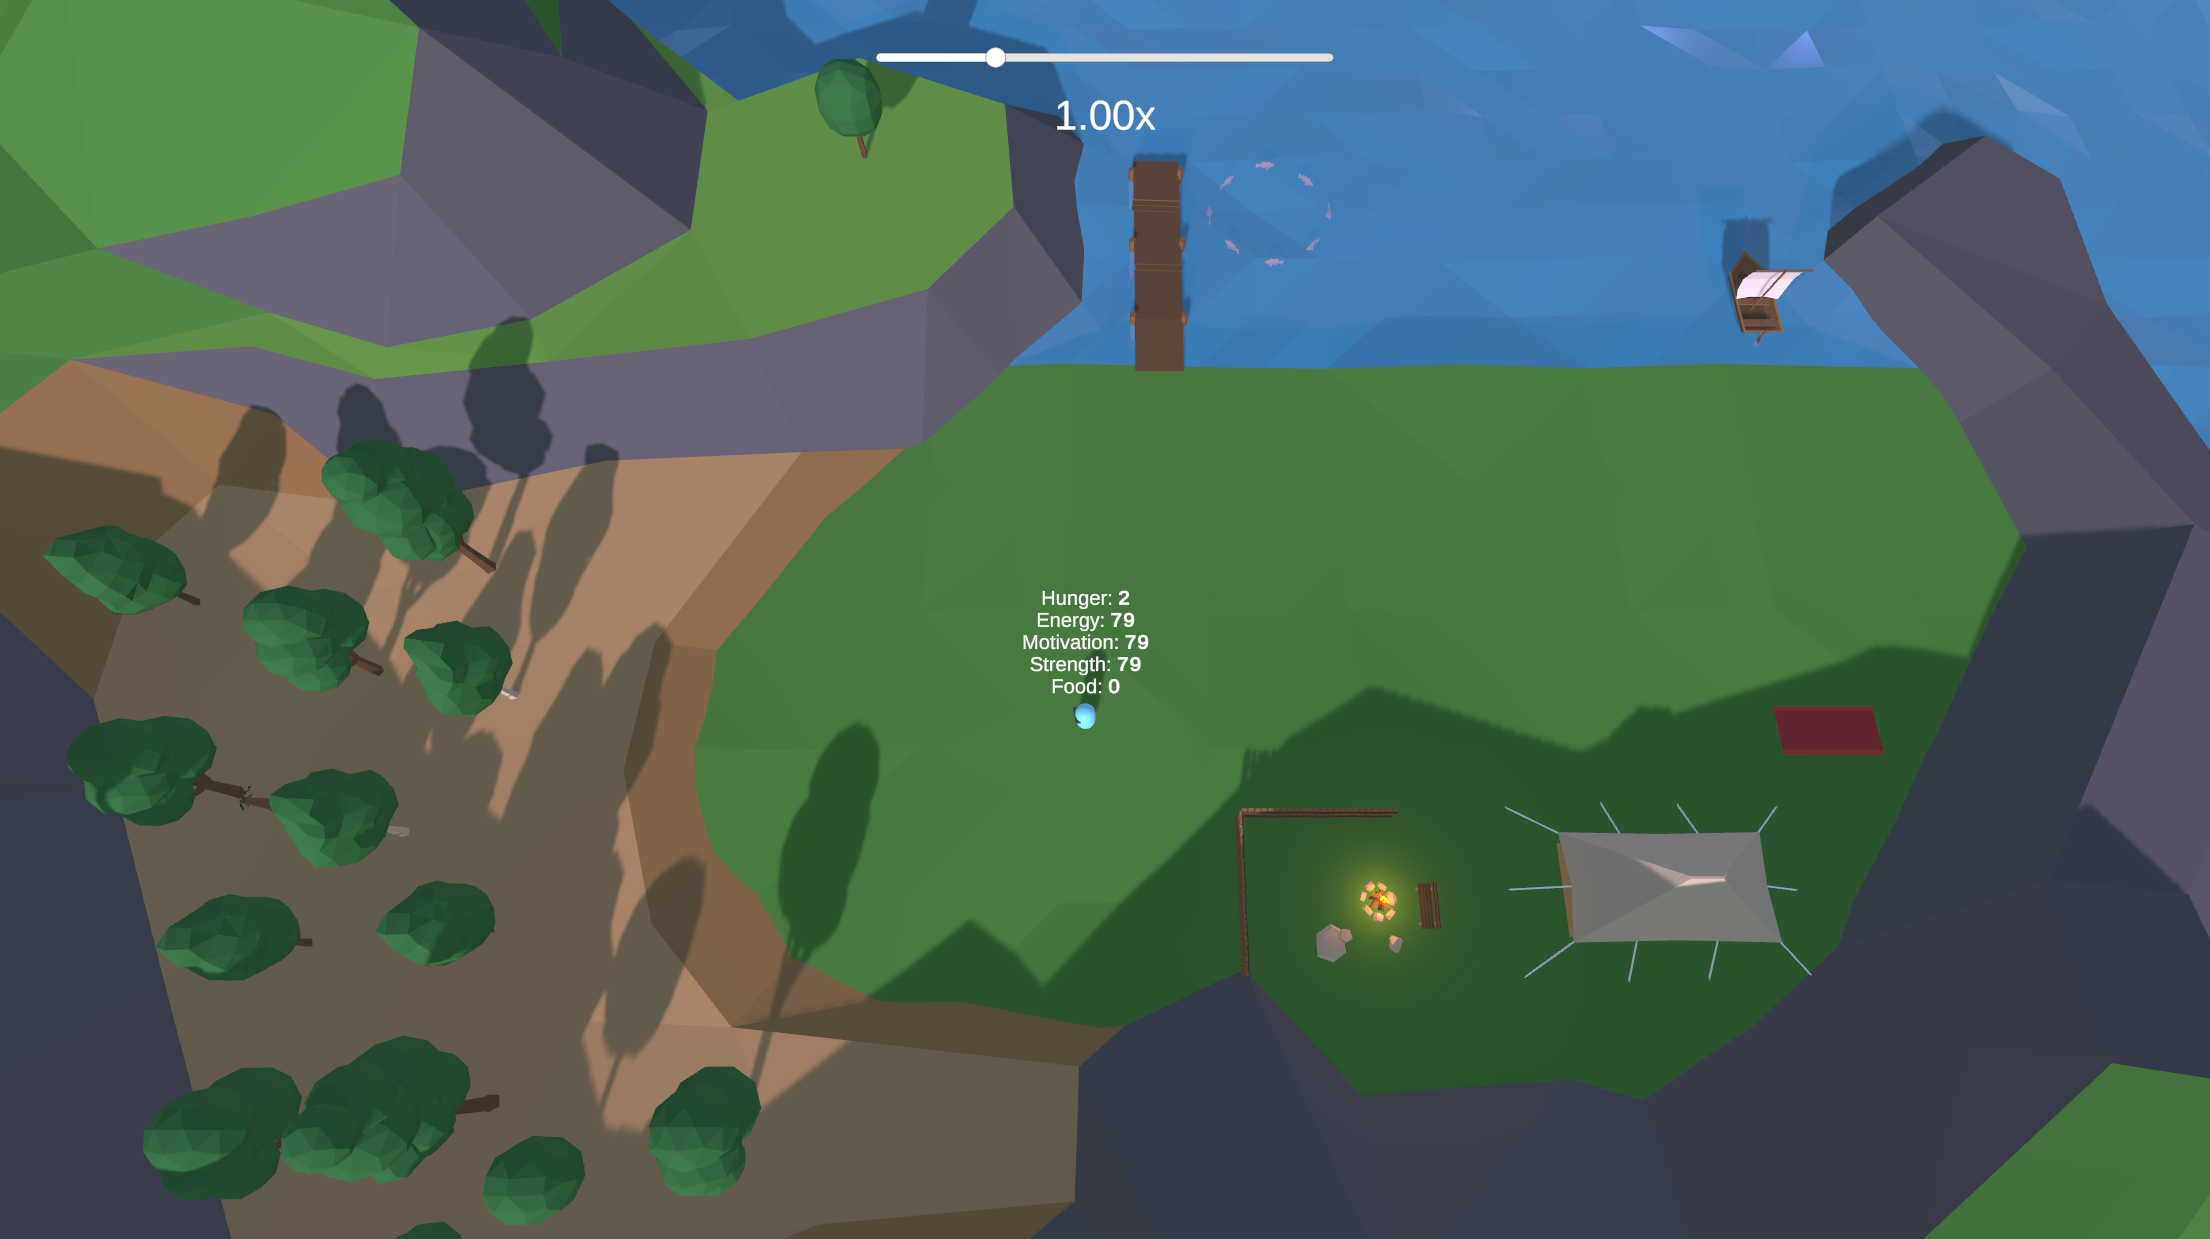
\includegraphics[scale=0.25]{images/utility_designer_survival.png}
	\caption{Survival scene in Unity}
	\label{fig:utility_designer_survival}
\end{figure}

\begin{figure}[H]
	\centering
		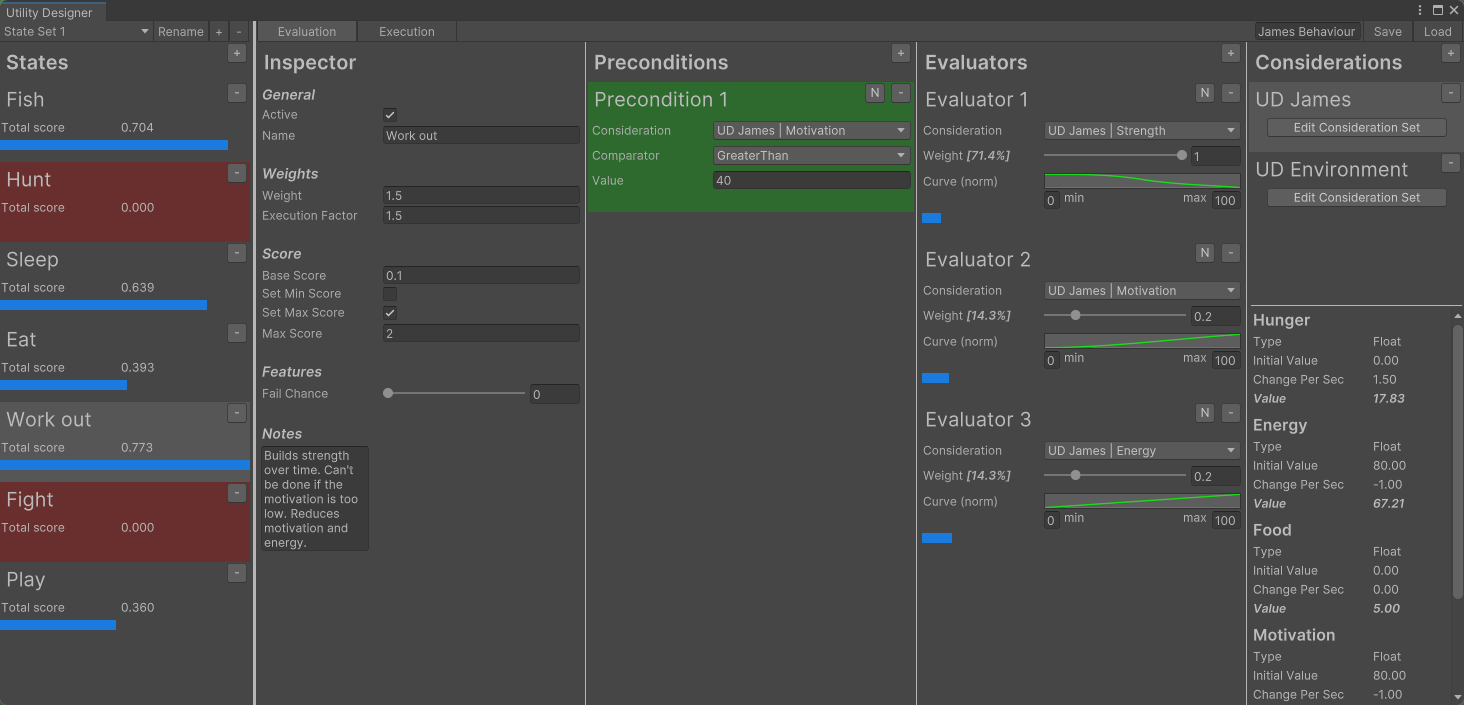
\includegraphics[scale=0.38]{images/utility_designer_survival_evaluation.png}
	\caption{Evaluation tab of Utility Designer}
	\label{fig:utility_designer_survival_evaluation}
\end{figure}

In the figure \ref{fig:utility_designer_daily_routine_evaluation}, the "Work out" state is currently selected and evaluated based on James' strength, motivation and energy. The most important factor for James is his own strength, as he would die from a bear attack if he was too weak. However, James does not like to train when he feels demotivated or tired, so evaluators 2 and 3 have a weight of 0.2. He also refuses to train when his motivation is very low, hence the precondition. The whole state is quite important, as he needs strength to survive a bear attack, which is represented by a weight of 1.5 and a base score of 0.1.

\begin{figure}[H]
	\centering
		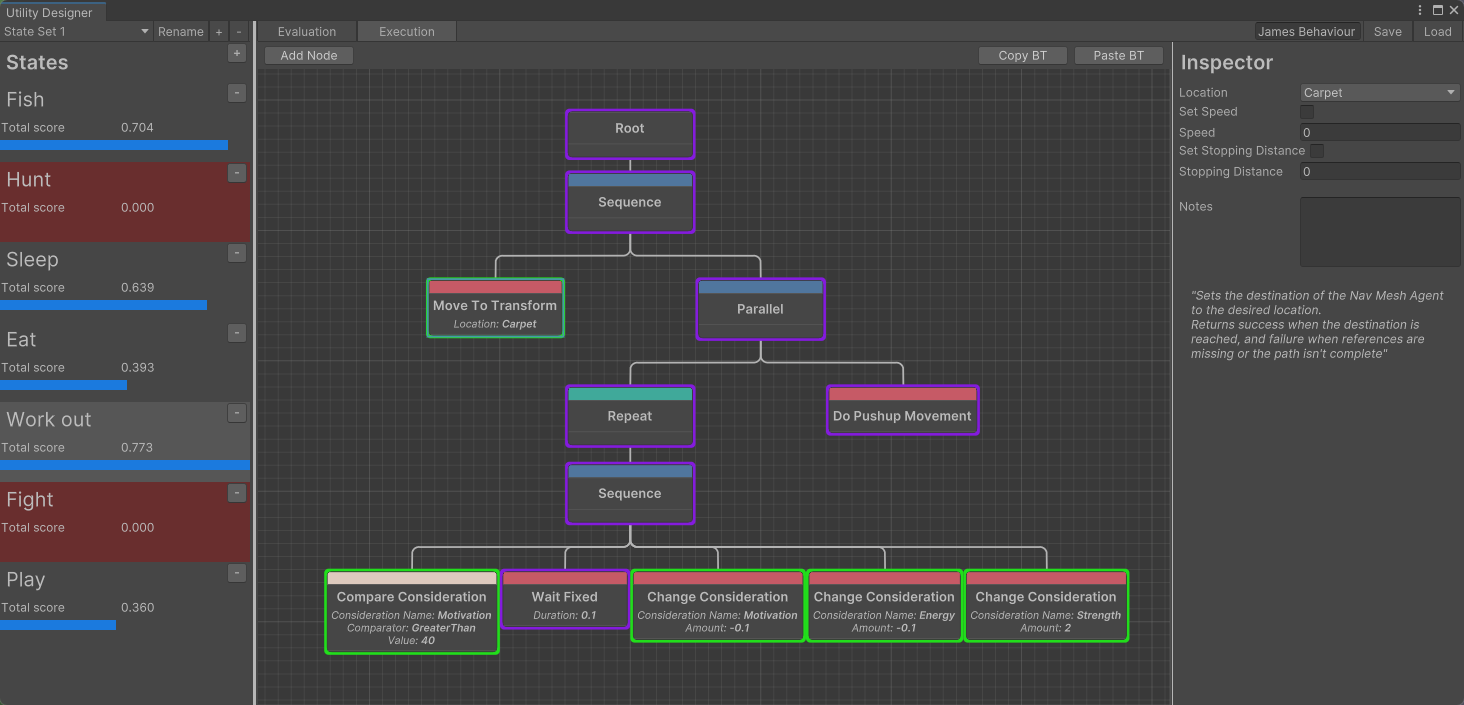
\includegraphics[scale=0.38]{images/utility_designer_survival_execution.png}
	\caption{Execution tab of Utility Designer}
	\label{fig:utility_designer_survival_execution}
\end{figure}

This shows the behaviour tree for the "Work out" state again. the first sequence is used to move to the carpet if it is not already there. Then the work out starts with a parallel node that allows the push up animation to be executed and the considerations to be changed in parallel. To the left of the sequence is a conditional node that checks whether James is motivated enough or not. This node is not really needed, as this condition is already checked in the evaluation tab, but it is here to show that such a check might also be possible in the behaviour tree. If this check is successful, the agent will gain 2 strength at a cost of 0.1 motivation and energy every 0.1s.

There were many variables that had to be set to make the NPC behave correctly, such as all the weights for the evaluators, adding preconditions, and configuring the inspector. But it was not as hard to configure as one might think, because everything can be done by intuition and simply thinking about the overall importance of each state and evaluator to get appropriate weights. Of course, some test runs were needed to fine-tune everything, which was also not too difficult due to the runtime debugging features.
\chapter{Performance}
\label{chap:performance}
\section{Computational Efficiency}
\label{sec:performance_computationalefficiency}

\subsection{Evaluation}
\label{sec:performance_computationalefficiency_evaluation}

In Utility Designer, the best state is decided at each evaluation tick. The tick rate can be set in the UtilityDesigner script and is clamped between 0.01s and 1s. Alternatively, Unity's update method can be used. This allows for a custom balance between the NPC's reaction time, in terms of switching to the right state faster, and performance. The question now is how expensive such an evaluation tick is:

On every evaluation tick, the code loops over all states. It immediately jumps to the next state if the state is not "Active". It loops over all preconditions and returns as soon as one of them is not met. Only when all preconditions are met does it loop over the evaluators to calculate their scores.

Scoring an evaluator means obtaining the current value of its curve based on its consideration. This score is then added to the base score, multiplied by its weights and clamped between the minimum and maximum scores if the appropriate switches are set. When it comes to calculating the weights for each evaluator, the calculation of the percentages only needs to be done once, at the start of the programme.

All states are ranked according to their score. After getting the best state, there is a chance that this state will not be chosen, based on the "Fail Chance". If the state fails, the next best state is chosen and the fail chance is also checked. This happens for all states until the state does not fail or it is the last state left. Since the states are already ordered, choosing the next best state just means looking at the next element in the list, and is therefore very efficient.

The considerations are also updated at the same tick rate, changing their value according to "Change Per Sec". They are always updated just before the evaluation takes place, to ensure that their value is up to date when the evaluation takes place.

\subsection{Execution}
\label{sec:performance_computationalefficiency_execution}

Similarly to the evaluation, the behaviour tree is updated on every execution tick, according to the settings in the UtilityDesigner script. It is also clamped between 0.01s and 1s, with the option to use Unity's Update method instead. A faster tick rate makes the NPC's behaviour more responsive, while a lower tick rate offers better performance.

\newpage

On each execution tick, the root node of the currently executing state is updated, all other behaviour trees of other states are ignored. Updating the behaviour tree does NOT mean looping over all nodes, it only updates the currently executing path. The composite node, which is the only node type that can have multiple children, caches the last child that returned Running. Each time the node is updated, it will only update the relevant child, without looking at the others. This is of course slightly different for the Parallel node, which can have multiple running children, and therefore needs to update them all on every tick.

\section{Profiling}
\label{sec:performance_profiling_profiling}

Unity provides a tool called the Profiler, which helps to analyse the efficiency of the game. To further test the performance of Utility Designer, the daily routine scene was populated with 1000 agents, each with their own local consideration set, but all sharing the same UtilityBehaviour. This means that they all make decisions on their own, but only share the same behaviour logic. The tick rate of the evaluation is set to 0.1s and for the execution tab it is set to Unity's Update method for each agent. An Intel Core i7 12700KF CPU was used for these tests.

\begin{figure}[H]
	\centering
		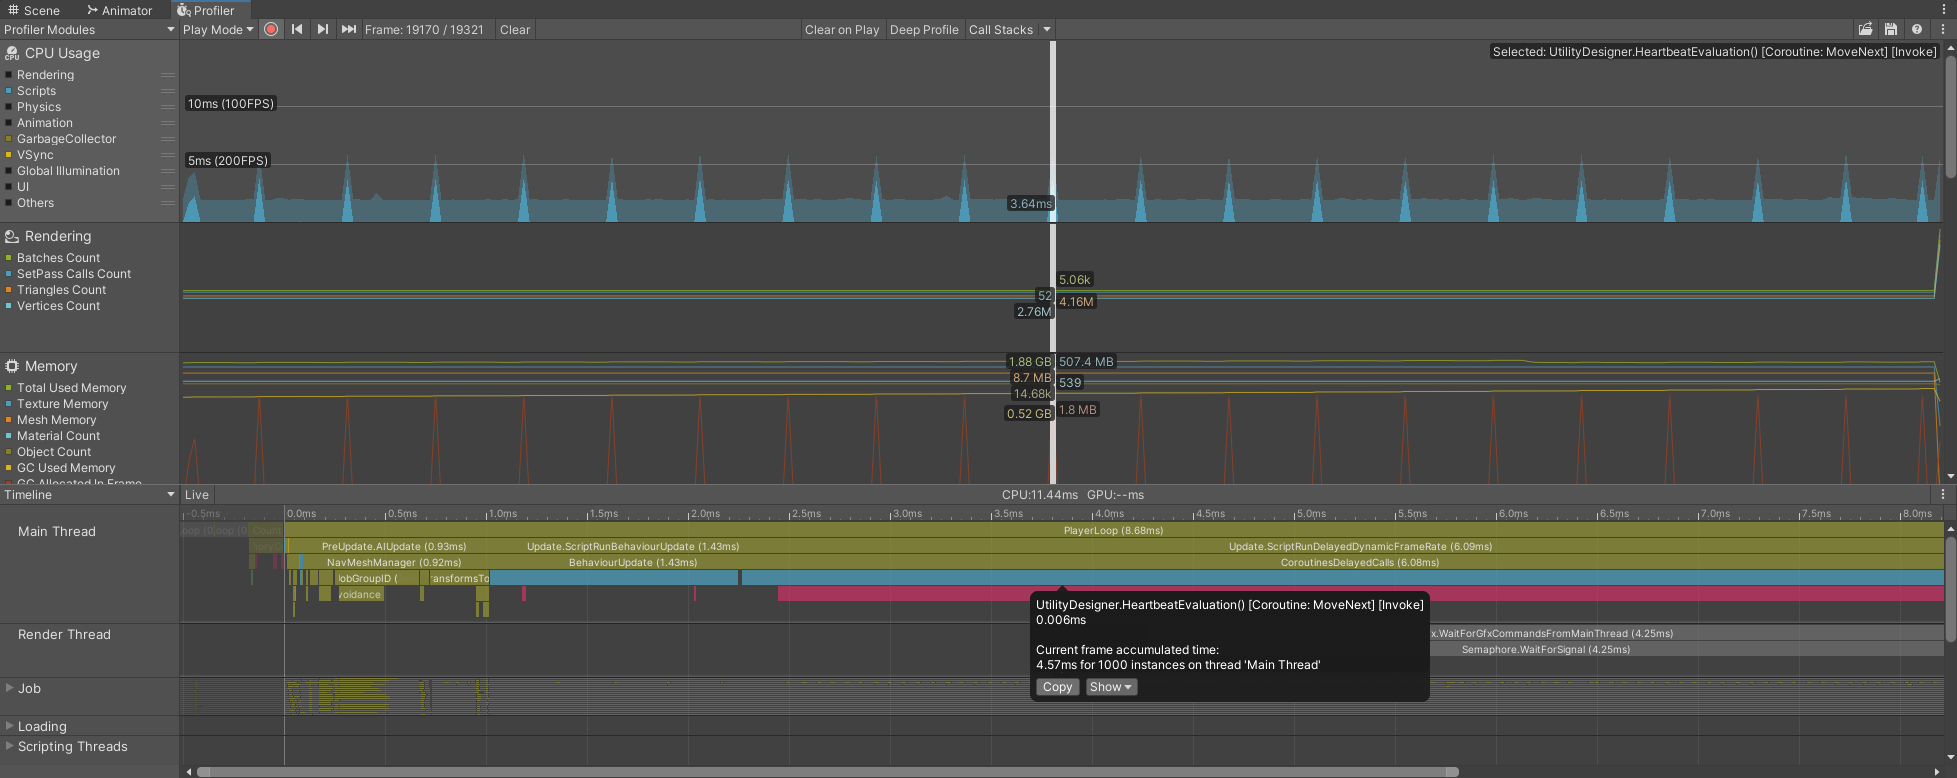
\includegraphics[scale=0.302]{images/utility_designer_profiling_1.png}
	\caption{Profiler with evaluation tick rate = 0.1s and execution tick rate = update}
	\label{fig:utility_designer_profiling_1}
\end{figure}

The first curve in light blue shows the CPU usage of the scripts. The tick rate of the evaluation tab is easy to see with spikes every 0.1s. Hovering over one of these spikes shows the exact time it takes to evaluate all 1000 agents in the main thread, which is 4.57ms. This time will change as states or evaluators are added or removed. Reducing the tick rates of Utility Designer will result in better performance:

\begin{figure}[H]
	\centering
		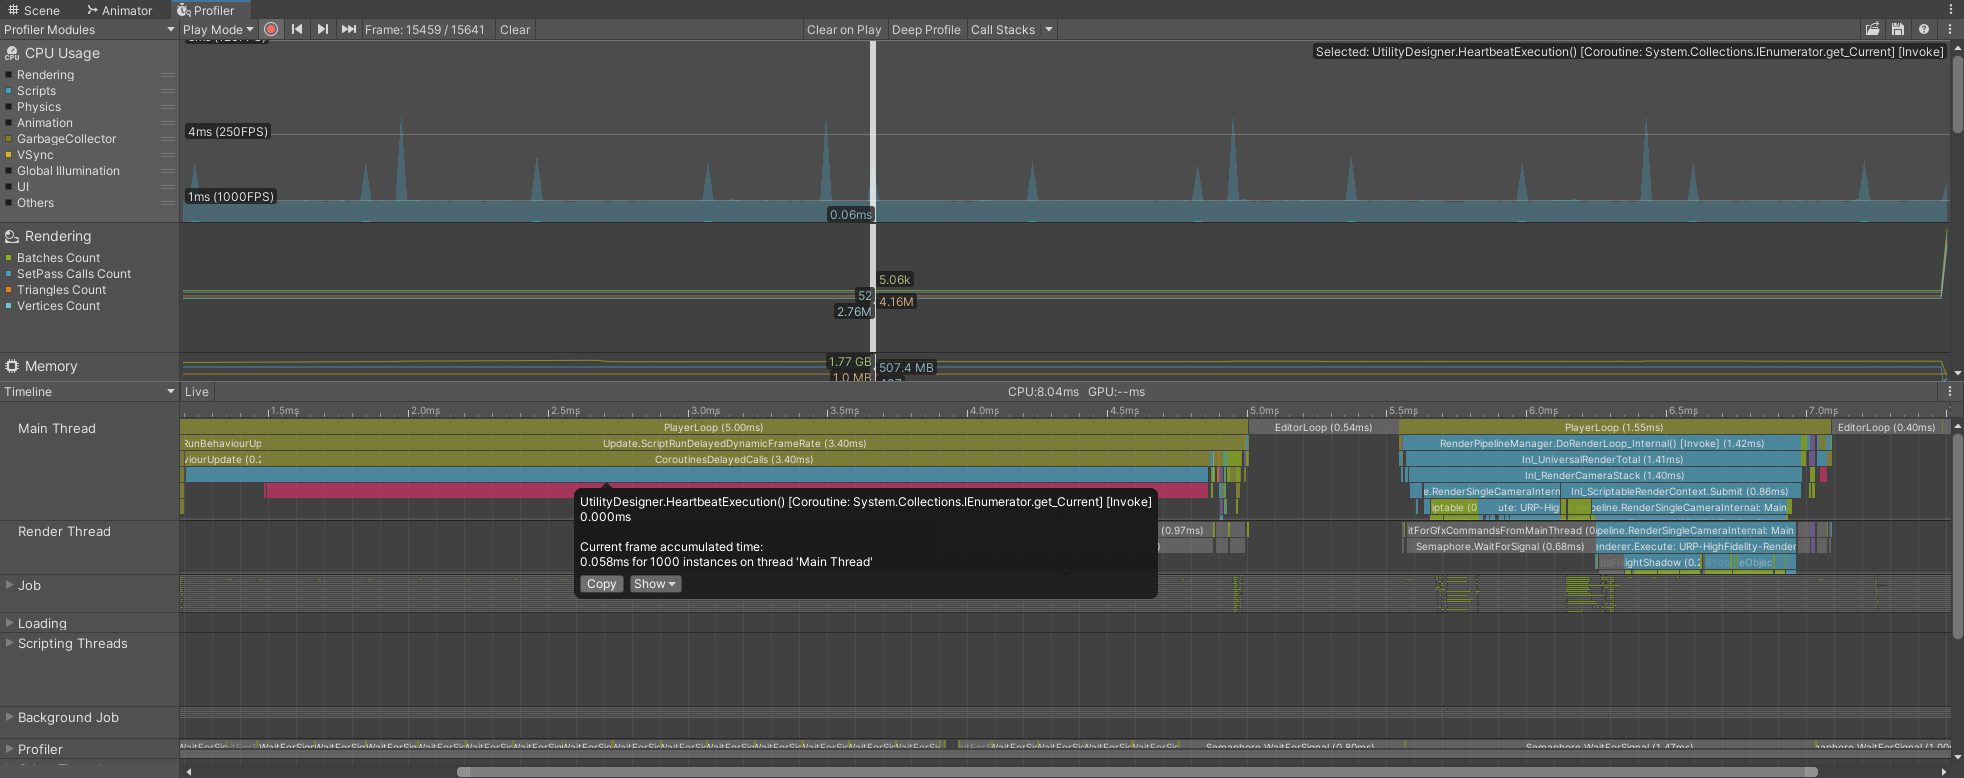
\includegraphics[scale=0.302]{images/utility_designer_profiling_2.png}
	\caption{Profiler with evaluation tick rate = 0.5s and execution tick rate = 0.2s}
	\label{fig:utility_designer_profiling_2}
\end{figure}

Looking at this example, it is clear that some performance can be gained by reducing the tick rates. The evaluation tick rate is set to 0.5s and is represented by the larger spike in figure \ref{fig:utility_designer_profiling_2}, while the execution tab is set to 0.2s and represents the smaller spikes. In the example of the daily routine scene, an execution tick is less expensive than an evaluation tick with a total of 0.058ms for 1000 agents. Overall, it still seems to be able to maintain a fairly high frame rate with 1000 fps down to around 200 fps at the exact time of the evaluation tick in the Unity editor. Often a built game will have an even higher frame rate than when running in the Unity editor.
\chapter{Next Steps}
\label{chap:nextsteps}
\section{Improvements}
\label{sec:nextsteps_improvements}

When creating a tool for other developers, it is important to keep everything as intuitive and simple as possible, while also supporting many different features to allow more flexibility. Decisions about how to implement certain functionality in Utility Designer were based on these criteria. However, because development time was limited, the focus had to be on the most important features, while others were not yet implemented.

If this project continues, here are some recommended features to consider implementing:

\paragraph{More Base Types:}
When creating a new consideration, there is an option to select its type. Currently there is only "float", but considerations should support more types like "int", "bool", etc. Implementing this is not a very quick task, as everything that uses considerations needs to be able to adapt to the specified type. For example, the curve for evaluators would work differently for a consideration of type "bool".

\paragraph{Inheritance:}
The concept of utility AI shines when it comes to creating multiple characters, all with the same set of states, but each with different priorities for each state. An example of this could be a civilisation simulation where each person has slightly different priorities for each action. This is currently possible by copying and pasting the Utility Behaviour, but adding, say, a new state to the world would mean adding that new state to each copied behaviour separately. Thus the idea of inheritance, where all NPCs would inherit from a base behaviour and then only need to adjust their weights according to their preferences. Consequently, any new state addition would only need to be implemented in the base behaviour itself.

\paragraph{Renaming:}
Currently, strings are used to access Consideration Sets and Considerations, representing their names. When renaming them, all occurrences in the code and also in the editor window have to be changed manually. An automatic way to rename them would therefore be useful.

\paragraph{Undo / Redo:}
Utility Designer doesn't support hotkeys to undo or redo actions. The cleanest way to implement this would probably be to use a SerializedObject, which would involve a lot of code refactoring.

\paragraph{Blackboard:}
In the context of a behaviour tree, a blackboard is a place where globally accessible data is stored and can be used by different nodes in the tree. It's essentially a data store that holds variables and information that different nodes within the behaviour tree can use to perform their tasks or make decisions. Utility Designer does not currently implement a blackboard, but it would be a nice feature to have, but it is not necessary for the core functionality of a behaviour tree.

\paragraph{Backwards Compatibility:}
The tool was created in Unity 2022, as the UI toolkit in this version is more stable than in previous versions. It is currently only compatible with the 2022 version, and making it compatible with earlier versions would make it available to a wider range of developers.

\section{Publishing To The Unity Asset Store}
\label{sec:nextsteps_publishtounityassetstore}

At the time of writing, the Utility Designer has been submitted to the Asset Store, but is still awaiting review by Unity. It has started at a queue position of \#2650, which means it will take about 30 working days for it to be reviewed. Once the asset has been reviewed and accepted, it will be available in the Unity Asset Store. It is possible that the asset will be rejected. In this case, further changes to the asset will be required before it can be resubmitted, depending on the reasons for the rejection.

The tool has been submitted as a free assets to increase the chances of getting more feedback from the community. This feedback can then be used to make improvements and to follow up with updates according to the feedback received or other changes as described in the previous section. The preview of the store page looks as follows:

\begin{figure}[H]
    \centering
    \begin{minipage}{0.49\textwidth}
        \centering
        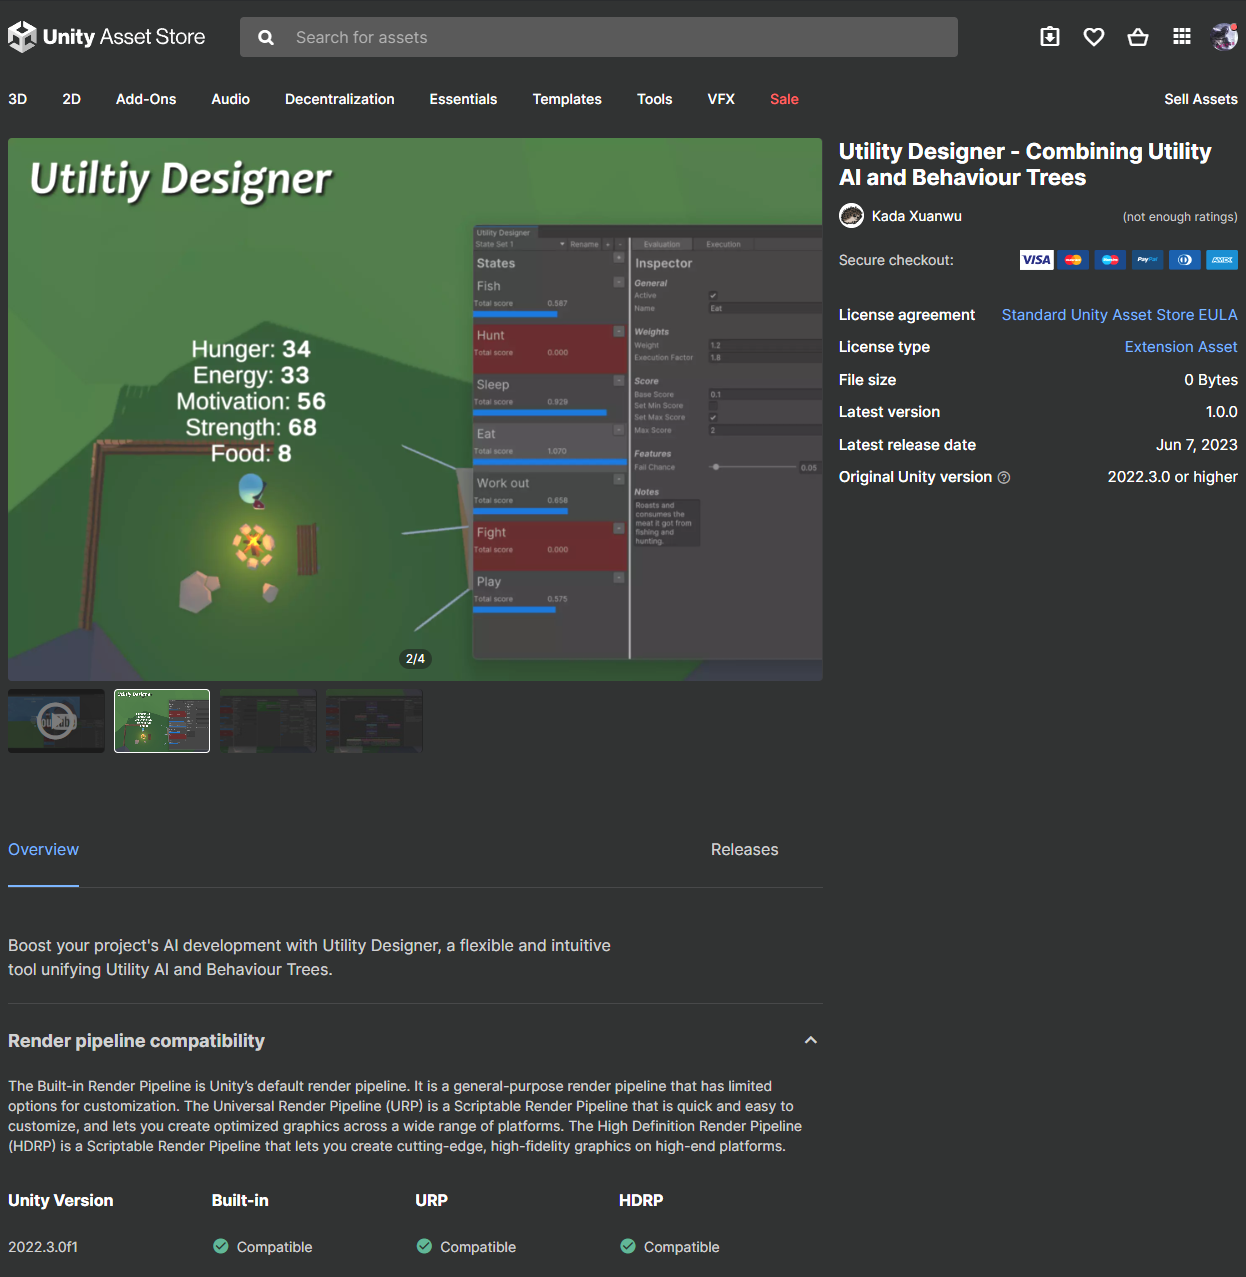
\includegraphics[scale=0.26]{images/asset_store_page_1.png}
        \caption{Asset Store Page Preview 1}
        \label{fig:asset_store_page_1}
    \end{minipage}\hfill
    \begin{minipage}{0.49\textwidth}
        \centering
        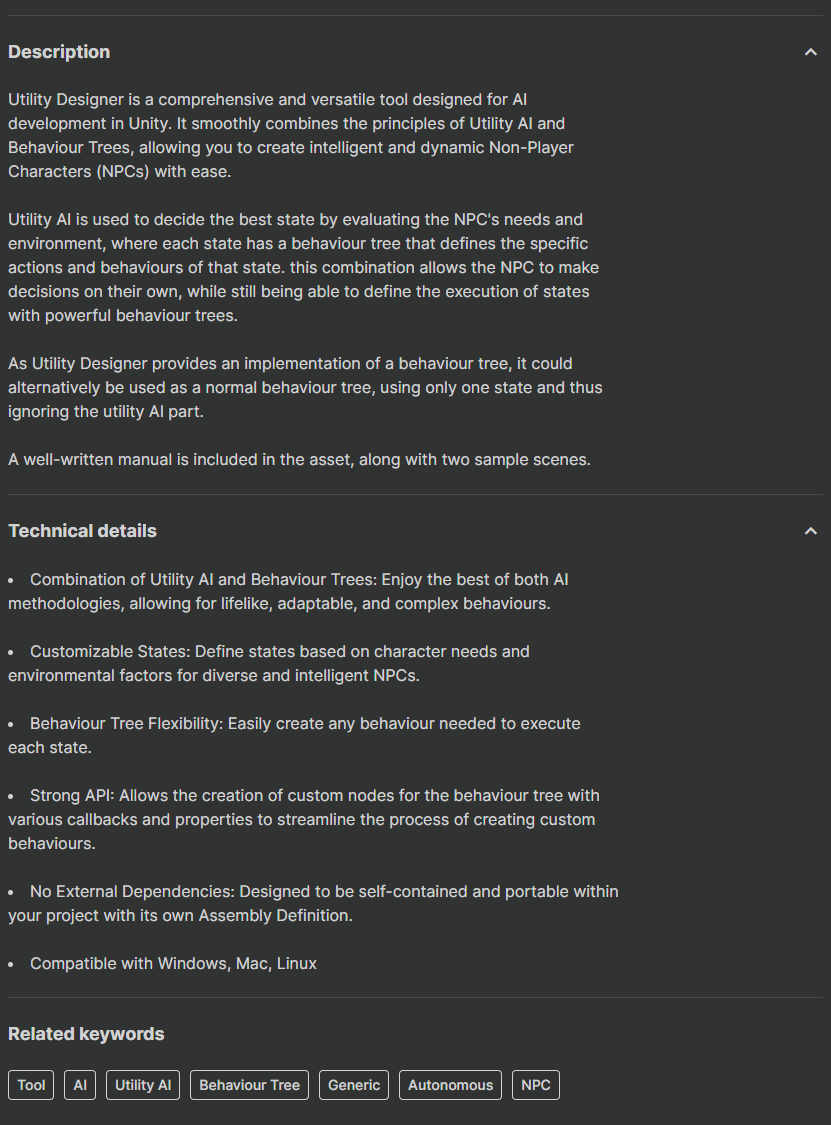
\includegraphics[scale=0.26]{images/asset_store_page_2.png}
        \caption{Page Preview 2}
        \label{fig:asset_store_page_2}
    \end{minipage}
\end{figure}

\newpage

There are several steps involved in preparing and publishing an asset, from asset preparation to submission and approval.

\paragraph{Preparing The Asset}

\begin{enumerate}
    \item \textbf{Asset Development:} The asset must be fully developed and working correctly, following Unity's best practices for asset development.
    \item \textbf{Documentation:} Comprehensive documentation should be provided for the asset. This should include clear instructions on how to use the asset and any known issues.
    \item \textbf{Testing:} The asset should be thoroughly tested to ensure that it works as expected.
\end{enumerate}

\paragraph{Packaging The Asset}

\begin{enumerate}
    \item \textbf{Organizing Files:} All files should be neatly organised in a clear folder structure. It is advisable to include an example folder containing at least one example scene and a documentation file.
    \item \textbf{Package Setup:} Unity provides an 'Export Package' option under the 'Assets' menu. This can be used to create a Unity package file (.unitypackage) of the asset.
\end{enumerate}

\paragraph{Submitting The Asset}

\begin{enumerate}
    \item \textbf{Creating A Publisher Account:} A Unity Publisher account is required to submit assets to the Unity Asset Store. The instructions on the Unity Asset Store can be followed to set up the account.
    \item \textbf{Asset Submission:} Once the Publisher account has been set up, the asset can be submitted for approval. This submission includes the necessary information such as the asset name, description, category, price and package file.
    \item \textbf{Images And Media:} High quality images and video should be provided to showcase the asset. This visual content is critical to marketing the asset to potential users.
    \item \textbf{Approval Wait Time:} The Unity team will review each submission. If approved, the asset becomes available for purchase in the Unity Asset Store. If not approved, Unity will provide feedback on what needs to be addressed. How long this process takes depends on the number of submissions they receive.
\end{enumerate}

\paragraph{After Approval}

\begin{enumerate}
    \item \textbf{Customer Support:} It is important to be prepared to provide support to customers. This support can include answering questions about the asset, providing updates and fixing bugs.
    \item \textbf{Updates And Maintenance:} Keeping the asset updated to ensure compatibility with the latest versions of Unity is critical. Addressing bugs promptly and incorporating user feedback into future updates is also essential.
\end{enumerate}

\chapter{Conclusion / Results}
\label{chap:conclusions}

When developing a tool, it is always important to know how the end user will feel when using it. The following insights were gained by creating two different test scenes and performance tests:

\begin{tabular}{lp{12cm}}
Development speed: & Once the basic concept of Utility Designer is clear, it was surprisingly fast to create new behaviours with it, as a new state can be created and configured with just a few clicks. Development speed starts to slow down when action nodes need to be implemented manually, so having a good selection of pre-built nodes helps save time. \cr
Maintenance: & Renaming considerations or even action nodes can sometimes be desirable, but the way Utility Designer is currently implemented makes it rather difficult to do so, as considerations for example are stored as strings. Adding and removing states, on the other hand, is very easy and can be done without having to think about other states, as they are all independent of each other. \cr
Flexibility: & The ability to use different preconditions and evaluators, to configure scoring in different ways, and the freedom to focus more on the utility AI or behaviour tree part makes the tool very flexible for different scenarios. Utility Designer can also be used as a normal behaviour tree, making it suitable even for scenarios where sequential behaviour is required, such as for a tour guide, where utility AI is not normally a good choice. \cr
Debugging: & One disadvantage of utility AI is that it is often difficult for developers to know exactly how the agent will behave. The runtime debugging features certainly help to analyse this, but the unpredictability still remains. This is not a major problem, as unpredictability is often desired in a utility AI system. \cr
Performance & Utility Designer does not seem to be problematic when it comes to performance, as the tests in section \ref{sec:performance_profiling_profiling} have shown. However, it is important to note that it becomes more expensive when there are many states and evaluators, and also when there is a fast tick rate, especially for the evaluation tab.
\end{tabular}

Overall, developing a tool has shown the many challenges of this task, such as the difficulty of making it easy and secure to maintain with all the different ways users can interact with it. There are also a lot of little things that make the whole development process take longer than one might think, as it requires tons of testing, creating sample scenes, writing good readable documentation, time to prepare it for the Unity Asset Store according to their guidelines, planning the layout and features, or even refactoring parts of the code based on test results.

\newpage

Using Utility Designer in action has shown that the concept of combining utility AI with a behaviour tree works really well together, offering the flexibility of independent states while retaining all the benefits of a behaviour tree. It can sometimes be a bit of a challenge to fine-tune all the weights in a utility AI system to make the agent act in the most efficient way possible. Interestingly, fine-tuning these weights could even be a task for machine learning to make it as good as possible. But the weights do not need to be perfect in most cases. Humans do not make perfect decisions all the time either, and if the weights are not set to the absolute optimum for every scenario, it might even help to represent the mistakes that humans make, thereby increasing realism.

As the Utility Designer is a tool made for the Asset Store, it is very likely that it will continue to be used after this thesis, depending on the feedback it receives from people using it. As it is being submitted as a free asset, there is a good chance that there will be a lot of feedback to implement.
%---------------------------------------------------------------------------

% Selbst�ndigkeitserkl�rung
%---------------------------------------------------------------------------
\cleardoublepage
\phantomsection 
\addcontentsline{toc}{chapter}{Declaration of authorship}
\chapter*{Declaration of primary authorship}
\label{chap:declaration_authorship}

\vspace*{10mm} 

I hereby confirm with my signature that I have independently carried out my present Bachelor's Thesis. All sources of information (technical literature, discussions with experts, etc.) and other aids that have significantly contributed to my work are fully listed in the appendix of my report. All contents that are not originated from me are marked with precise references to their sources.

\vspace{15mm}

\begin{tabbing}
xxxxxxxxxxxxxxxxxxxxxxxxxxxxxx\=xxxxxxxxxxxxxxxxxxxxxxxxxxxxxx\=xxxxxxxxxxxxxxxxxxxxxxxxxxxxxx\kill
Place, Date:		\> Grasswil, \versiondate \\ \\ 
Last Name, First Name:	\> K\"aser David \\ \\ \\ \\ 
Signature:	\> ......................................\>
\end{tabbing}

%---------------------------------------------------------------------------

% Glossary
%---------------------------------------------------------------------------
%\cleardoublepage
%\phantomsection 
%\addcontentsline{toc}{chapter}{Glossay}
%\renewcommand{\glossaryname}{Glossay}
%\printglossary
%---------------------------------------------------------------------------

% Bibliography
%---------------------------------------------------------------------------
\cleardoublepage
\phantomsection 
\addcontentsline{toc}{chapter}{Bibliography}
\bibliographystyle{IEEEtranS}
\bibliography{database/bibliography}{}
%---------------------------------------------------------------------------

% Listings
%---------------------------------------------------------------------------
\cleardoublepage
\phantomsection 
\addcontentsline{toc}{chapter}{List of figures}
\listoffigures
%\cleardoublepage
%\phantomsection 
%\addcontentsline{toc}{chapter}{List of tables}
%\listoftables
%---------------------------------------------------------------------------

% Index
%---------------------------------------------------------------------------
\cleardoublepage
\phantomsection 
\addcontentsline{toc}{chapter}{Index}
\printindex
%---------------------------------------------------------------------------

% Attachment:
%---------------------------------------------------------------------------
\appendix
\settocdepth{section}
\chapter*{APPENDICES}
\addcontentsline{toc}{chapter}{APPENDICES}

\begingroup\let\clearpage\relax
\chapter{Requirement Specification}
\label{chap:requirement_specification}
\endgroup

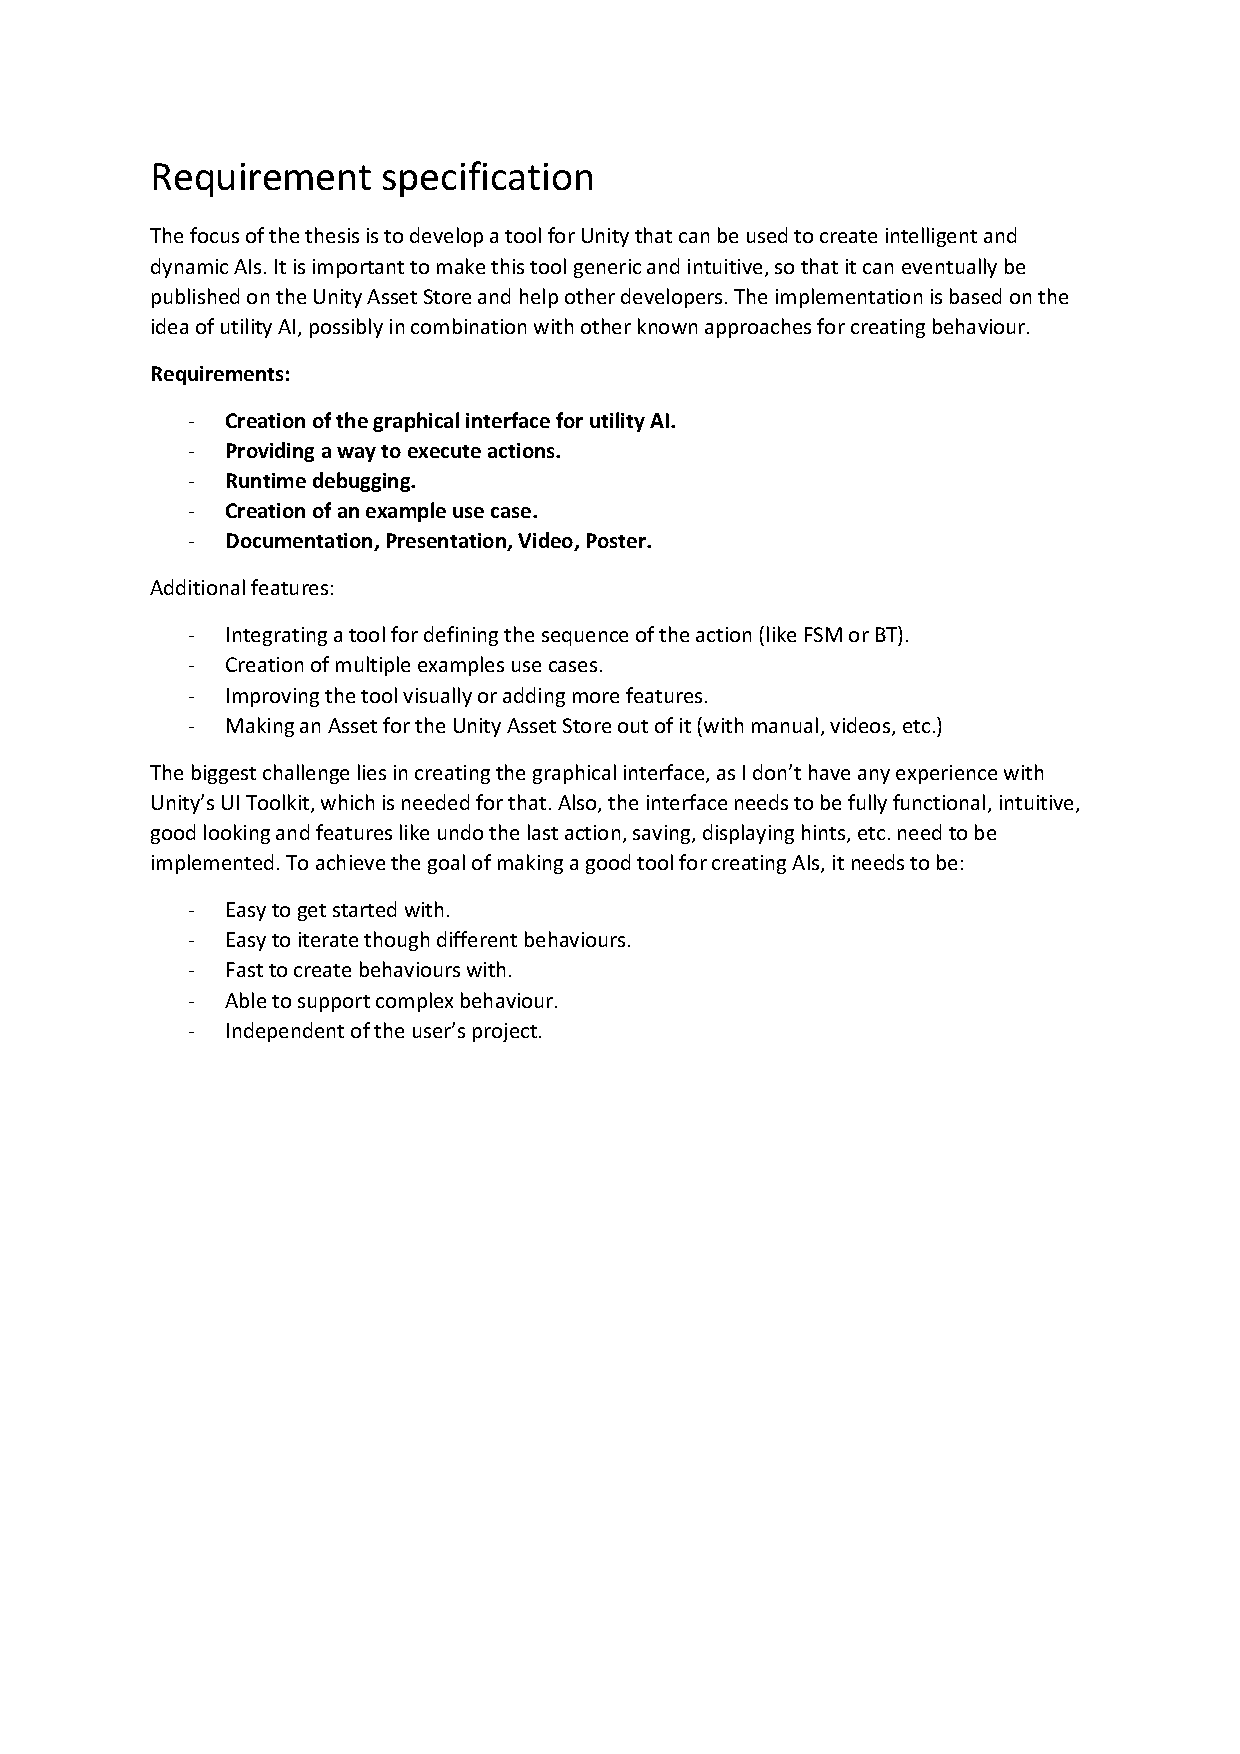
\includepdf[pages=-,scale=0.9,pagecommand={}]{database/requirement_specification.pdf}
\chapter{Git Repository}
\label{chap:appendix_stories}

\section{Link}

The project can be found here: https://gitlab.ti.bfh.ch/kaesd4/utilityai

\section{Read Me}

This git repository contains the LaTeX documentation associated with this thesis, as well as a Unity project (compatible with Unity version 2022) that includes the implementation developed for this thesis.

Inside the Assets directory, a folder named KadaXuanwu can be found, which contains the asset that has been submitted to the Unity Asset Store. This asset includes three Unity packages which can be imported to obtain two example scenes. One package contains scenes for the Built-In Render Pipeline, another for the Universal Render Pipeline (URP), and the last one for the High Definition Render Pipeline (HDRP). Remember to also import Unity's "AI Navigation" package before running the sample scenes, as it is needed for pathfinding.

Outside of the KadaXuanwu directory, there is a Scenes folder that contains an additional example scene. This scene is identical to the Survival scene found in the Utility Designer examples, but with enhanced visual assets. It couldn't be bundled with the Utility Designer asset because the low-poly prefabs are sourced from a different asset.
\chapter{Stories}
\label{chap:appendix_stories}

At the beginning of Projects 2, some stories were written to figure out the flexibility needed in a tool that would provide an interface for creating generic behaviour.

\section{Tour Guide For Aventicum VR}

\begin{itemize}
    \item Tourguide waits for the visitors to arrive.
    \item While waiting, he waves at the visitors.
    \item When the visitors are close enough, he starts his welcome speech.
    \item After finishing his speech, he starts walking towards Location 1.
    \item After everyone has reached Location 1, he starts to talk again.
    \item While talking, he points at the building and steps a bit to the side (away from the tourists).
    \item After finishing his speech, he starts walking towards Location 2.
    \item This time, he also says something while walking and while everyone is close enough.
    \item After everyone has reached Location 2, he starts to talk again.
    \item After finishing his speech, the tour ends.
    \item At any time the tourguide is talking or walking and the visitors are too far away, he will pause and wave at them.
\end{itemize}

\section{Zombie Apocalypse}

\begin{itemize}
    \item 10 Zombies are trying to bite the player.
    \item They walk towards the player at a given speed.
    \item 5 of them will stay grouped and are a bit faster than the other 5.
    \item Zombies always keep a small gap between each other.
    \item Zombies become faster the less health they have.
    \item A friendly NPC (Bot) helps the player to kill the zombies, using a gun.
    \item The NPC tries to keep as much distance as possible to the zombies, while still staying in range to shoot at them (gun has a max range of 40 meters).
    \item The NPC needs to maintain line of sight to the zombies, and will reposition if it breaks.
    \item The NPC forgets the position of the zombies when he doesn't see them for more than 5 seconds, and will enter a patrolling state.
\end{itemize}

\section{Escort Quest}

In a role-playing game, there are various NPCs who must follow the player for certain quests. While following, the NPCs may be able to help fight monsters attacking the player, or they may be scared and stay back. Also, the NPC may prefer to walk on the road rather than the grass.

\begin{itemize}
    \item \textbf{Father:}
    \begin{itemize}
        \item Engages in aggressive combat against the monsters to protect the family.
        \item Unafraid of sacrificing himself for his family.
        \item Prefers walking on the road.
    \end{itemize}

    \item \textbf{Mother:}
    \begin{itemize}
        \item Helps fight the monsters, but primarily to defend the child.
        \item Will attempt to retreat when facing a strong monster, provided the child is safe.
        \item Prefers walking on the road, but always remains close to the child.
    \end{itemize}

    \item \textbf{Child:}
    \begin{itemize}
        \item Fearful of monsters and will only fight if there is no avenue for escape.
        \item Seeks safety by staying close to her mother.
        \item Prefers to play and run in the grass, avoiding the road.
    \end{itemize}
\end{itemize}

This example illustrates the complexity and nuance of character behaviour that game developers often need to create in order to immerse the player in a rich, believable world.

\section{Defending NPC}

Enemy Bot trying to defend his area by shooting at us. Usually he walks around in his paroling area. When he detects the player, he will switch to combat state and try to defeat us until we are dead or too far away from him.

The player can be detected through multiple ways: [FOV, sound, hints like dead bodies]
FOV and sound both depend on distance.
The more hints he has, the more likely he is to enter searching / combat state.

While in combat state, he ...
\begin{itemize}
    \item ... has different actions: [heal, attack, cover, re-position, reload, flee]
    \item ... has different attacks: [sniper, shotgun, knife]
\end{itemize}

Every action has a different curve for each variable and a weight for it. Examples for that could be:

\begin{itemize}
    \item Heal: factor 10
    \item Enemy Health: factor 2
    \item Current ammo: factor 3
\end{itemize}
\chapter{Timetable}
\label{chap:appendix_timetable}
\newpage

\begin{figure}[H]
	\centering
		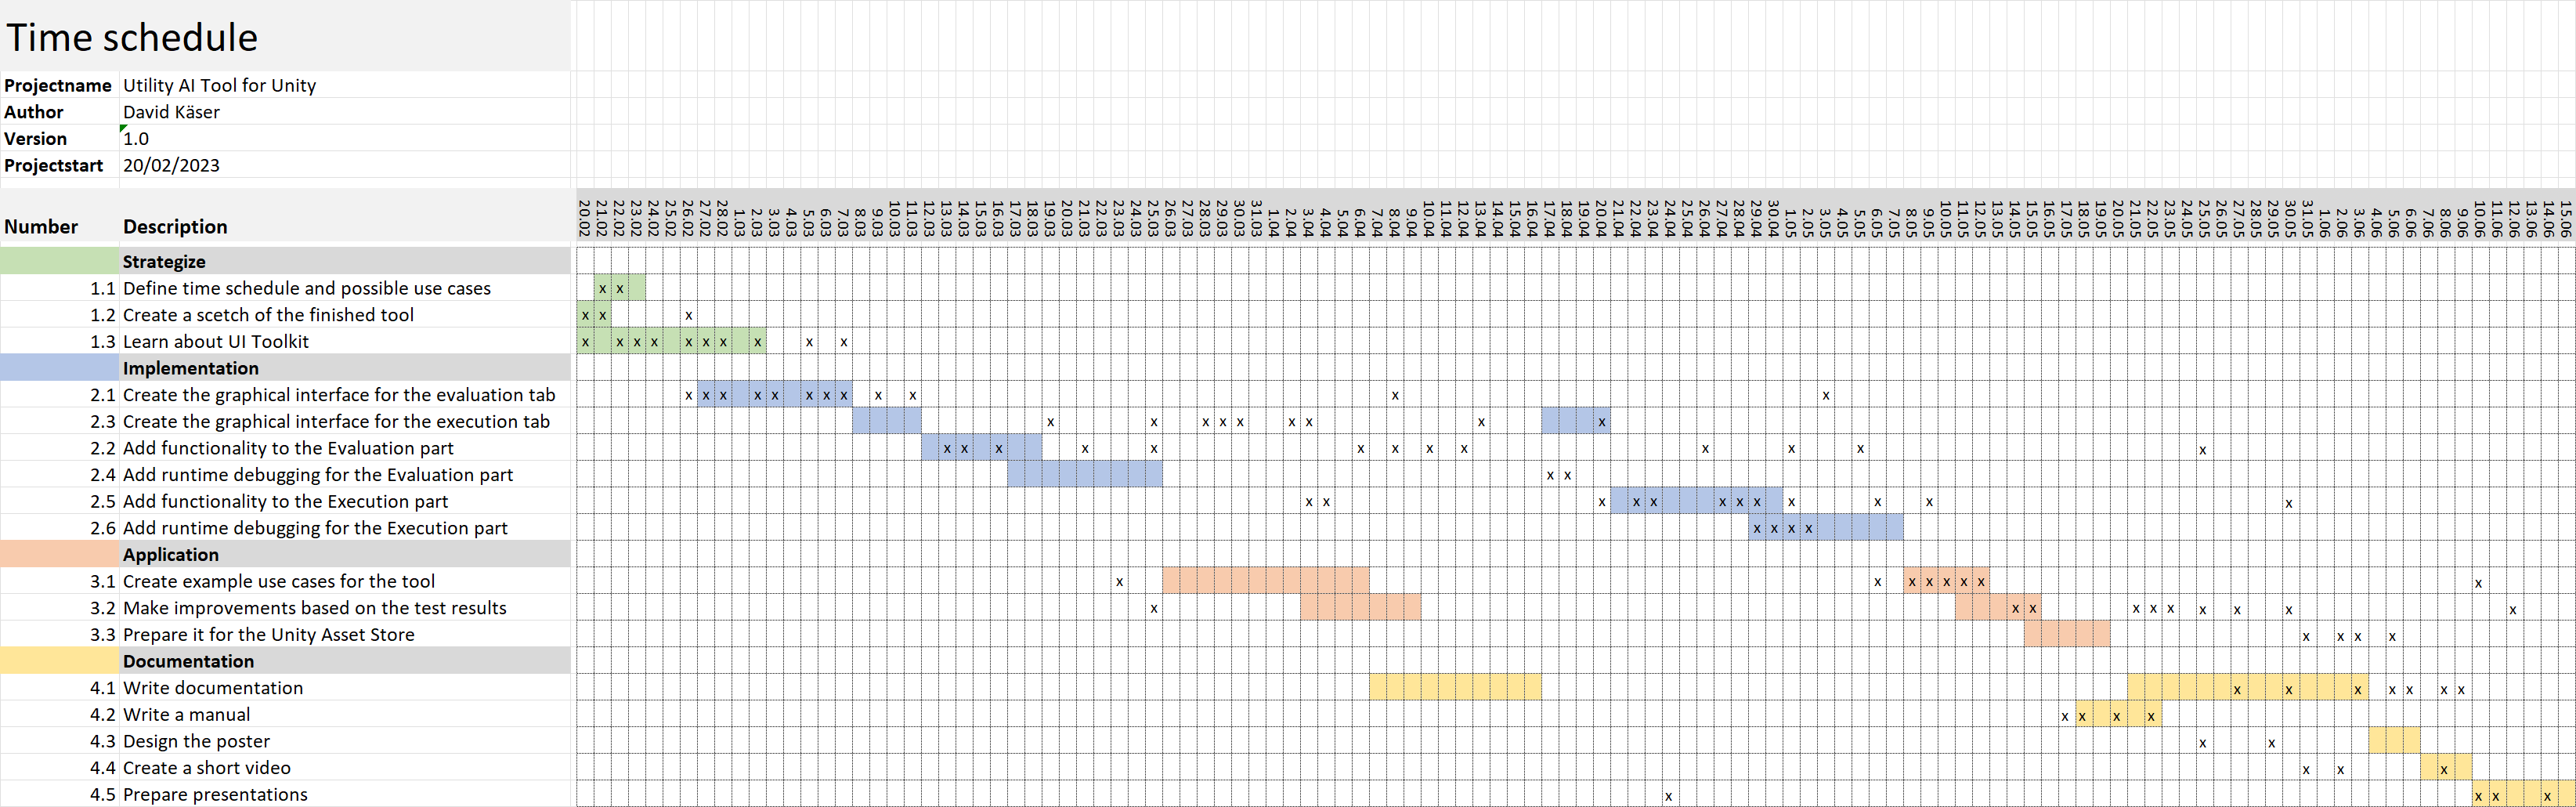
\includegraphics[scale=0.28, angle=90]{images/timetable.png}
	\caption{Timetable made at the start of the project}
	\label{fig:timetable}
\end{figure}

\chapter{Utility Designer Manual}
\label{chap:appendix_utilitydesignermanual}

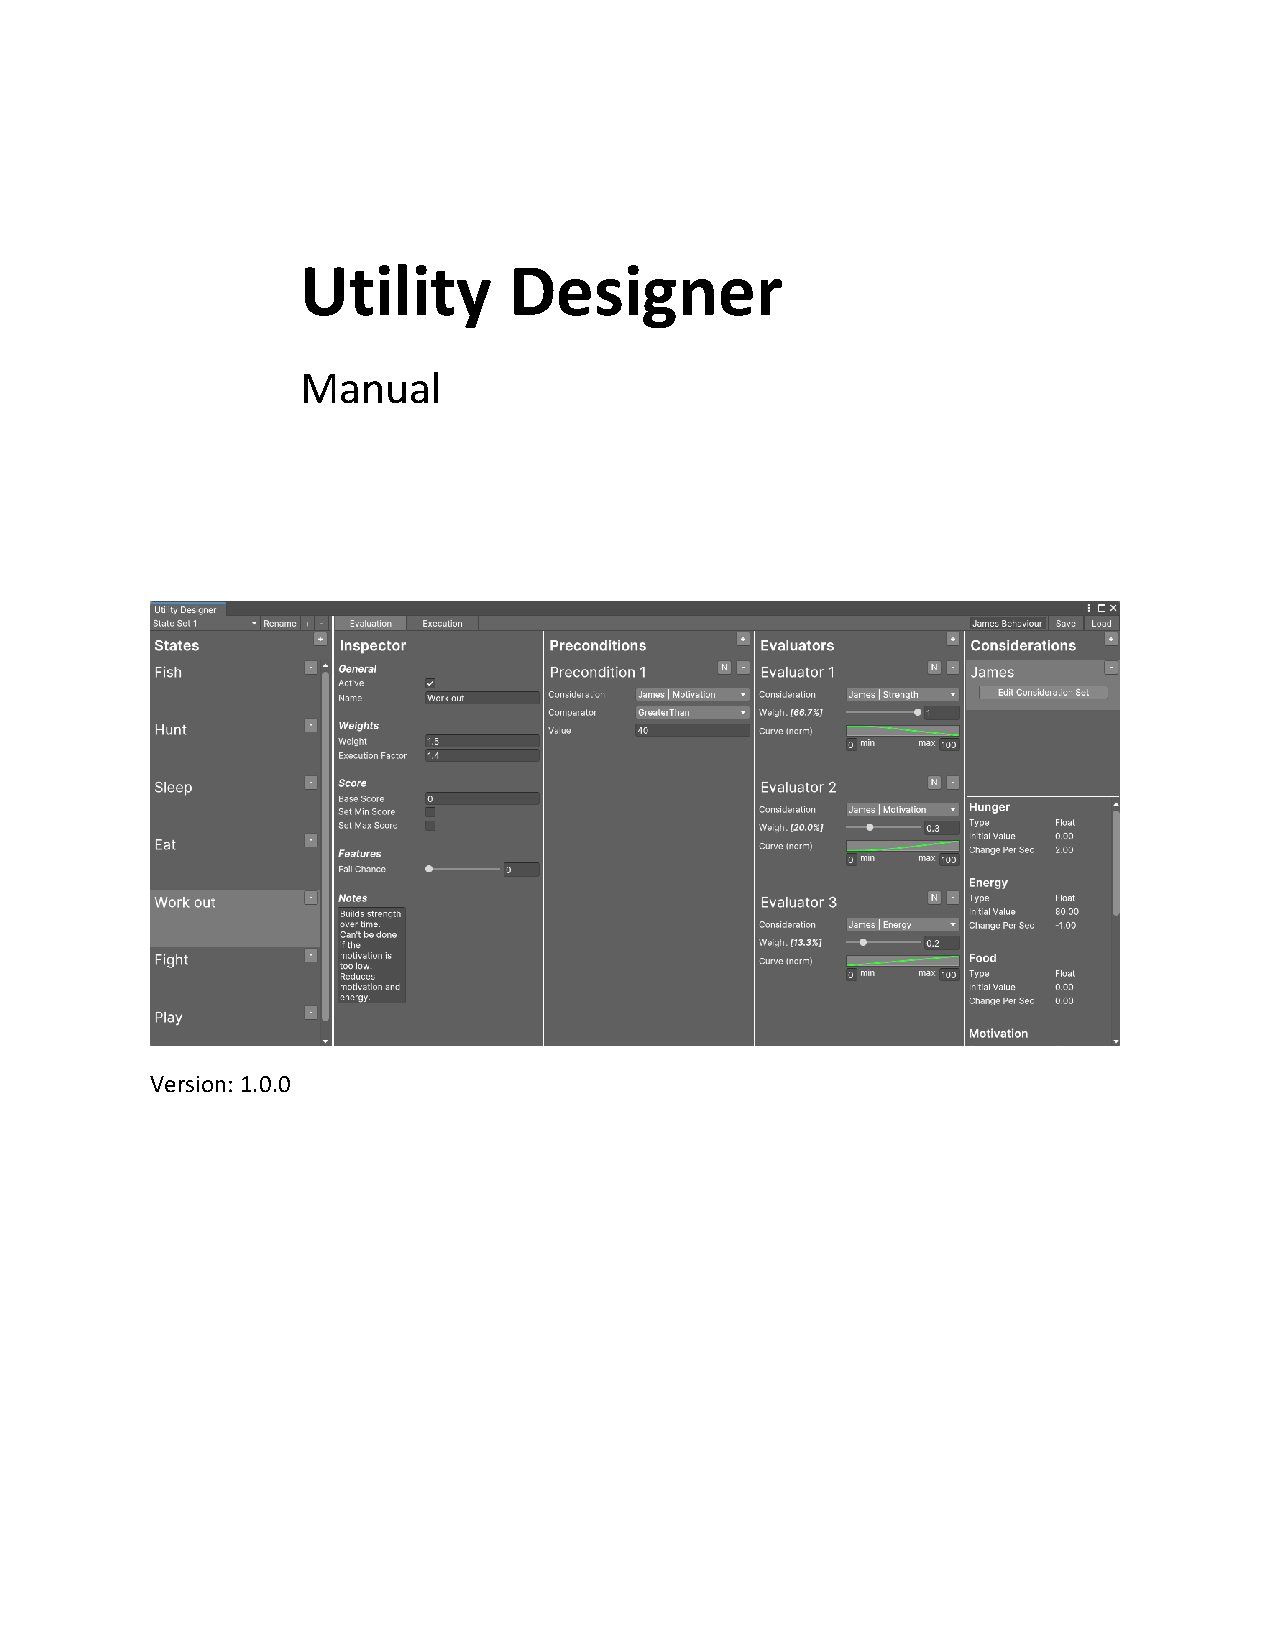
\includepdf[pages=-,scale=0.9,pagecommand={}]{database/utility_designer_manual.pdf}
%\chapter*{APPENDICES}
\addcontentsline{toc}{chapter}{APPENDICES}

\begingroup\let\clearpage\relax
\chapter{Arbitrary Appendix}
\label{chap:appendix_arb}
\endgroup

The European languages are members of the same family. Their separate existence is a myth. For science, music, sport, etc, Europe uses the same vocabulary. The languages only differ in their grammar, their pronunciation and their most common words. Everyone realizes why a new common language would be desirable: one could refuse to pay expensive translators. To achieve this, it would be necessary to have uniform grammar, pronunciation and more common words. If several languages coalesce, the grammar of the resulting language is more simple and regular than that of the individual languages. The new common language will be more simple and regular than the existing European languages. It will be as simple as Occidental; in fact, it will be Occidental. 
%\chapter{Additional Appendix}
\label{chap:appendix_B}

\section{Test 1}
To an English person, it will seem like simplified English, as a skeptical Cambridge friend of mine told me what Occidental is. The European languages are members of the same family. Their separate existence is a myth. For science, music, sport, etc, Europe uses the same vocabulary. The languages only differ in their grammar, their pronunciation and their most common words. Everyone realizes why a new common language would be desirable: one could refuse to pay expensive translators. To achieve this, it would be necessary to have uniform grammar, pronunciation and more common words. If several languages coalesce, the grammar of the resulting language is more simple and regular than that of the individual languages. The new common language will be more simple and regular than the existing European languages. 

\subsection{Environment}
It will be as simple as Occidental; in fact, it will be Occidental. To an English person, it will seem like simplified English, as a skeptical Cambridge friend of mine told me what Occidental is. The European languages are members of the same family. Their separate existence is a myth. For science, music, sport, etc, Europe uses the same vocabulary. The languages only differ in their grammar, their pronunciation and their most common words. Everyone realizes why a new common language would be desirable: one could refuse to pay expensive translators. To achieve this, it would be necessary to have uniform grammar, pronunciation and more common words.
%\chapter{Content of CD-ROM}
\label{chap:appendix_CDROM}

Content of the enclosed CD-ROM, directory tree, etc.
%---------------------------------------------------------------------------

%---------------------------------------------------------------------------
\end{document}

